\documentclass[submission,copyright,creativecommons]{eptcs}
\providecommand{\event}{AiML 2026} 

% AiML macros (for writing theorems)
\usepackage{aiml26}

\usepackage{iftex}
\ifpdf
    \usepackage{underscore}                 % Only needed if you use pdflatex.
    \usepackage[T1]{fontenc}                % Recommended with pdflatex
\else
    \usepackage{breakurl}                     % Not needed if you use pdflatex only.
\fi

\usepackage{tikz}
\usepackage{xspace}
\usepackage{amsmath}
\usepackage{amsthm}
\usepackage{standalone}
\usepackage{bm}


%\input{derivmacros}
%% Letters %%%%%%%%%%%%%%%%%%%%%%%%%%

\def\tA{\tilde{A}}
\def\tB{\tilde{B}}
\def\tC{\tilde{C}}
\def\tP{\tilde{P}}
\def\tQ{\tilde{Q}}
\def\tR{\tilde{R}}
\def\tS{\tilde{S}}
\def\tT{\tilde{T}}
\def\tU{\tilde{U}}
\def\tW{\tilde{W}}
\def\tDelta{\tilde{\Delta}}
\def\tGamma{\tilde{\Gamma}}
\def\tPi{\tilde{\Pi}}
\def\tpi{\tilde{\pi}}
\def\tsigma{\tilde{\sigma}}
\def\ts{\tilde{s}}

\def\ha{\hat{a}}

\def\hA{\hat{A}}
\def\hB{\hat{B}}
\def\hP{\hat{P}}
\def\hQ{\hat{Q}}
\def\hR{\hat{R}}
\def\hS{\hat{S}}
\def\hT{\hat{T}}
\def\hW{\hat{W}}
\def\hDelta{\hat{\Delta}}
\def\hGamma{\hat{\Gamma}}
\def\hrho{\hat{\rho}}
\def\hphi{\hat{\phi}}
\def\hpsi{\hat{\psi}}
\def\vphi{\check{\phi}}

\def\cA{{\mathcal A}}
\def\cB{{\mathcal B}}
\def\cC{{\mathcal C}}
\def\cD{{\mathcal D}}
\def\cE{{\mathcal E}}
\def\cF{{\mathcal F}}
\def\cG{{\mathcal G}}
\def\cH{{\mathcal H}}
\def\cI{{\mathcal I}}
\def\cJ{{\mathcal J}}
\def\cK{{\mathcal K}}
\def\cL{{\mathcal L}}
\def\cM{{\mathcal M}}
\def\cN{{\mathcal N}}
\def\cO{{\mathcal O}}
\def\cP{{\mathcal P}}
\def\cQ{{\mathcal Q}}
\def\cR{{\mathcal R}}
\def\cS{{\mathcal S}}
\def\cT{{\mathcal T}}
\def\cU{{\mathcal U}}
\def\cV{{\mathcal V}}
\def\cW{{\mathcal W}}
\def\cX{{\mathcal X}}
\def\cY{{\mathcal Y}}
\def\cZ{{\mathcal Z}}

\newcommand{\fA}{{\mathfrak A}}
\newcommand{\fB}{{\mathfrak B}}
\newcommand{\fC}{{\mathfrak C}}
\newcommand{\fD}{{\mathfrak D}}
\newcommand{\fE}{{\mathfrak E}}
\newcommand{\fF}{{\mathfrak F}}
\newcommand{\fG}{{\mathfrak G}}
\newcommand{\fH}{{\mathfrak H}}
\newcommand{\fI}{{\mathfrak I}}
\newcommand{\fJ}{{\mathfrak J}}
\newcommand{\fK}{{\mathfrak K}}
\newcommand{\fL}{{\mathfrak L}}
\newcommand{\fM}{{\mathfrak M}}
\newcommand{\fN}{{\mathfrak N}}
\newcommand{\fO}{{\mathfrak O}}
\newcommand{\fP}{{\mathfrak P}}
\newcommand{\fQ}{{\mathfrak Q}}
\newcommand{\fR}{{\mathfrak R}}
\newcommand{\fS}{{\mathfrak S}}
\newcommand{\fT}{{\mathfrak T}}
\newcommand{\fU}{{\mathfrak U}}
\newcommand{\fV}{{\mathfrak V}}
\newcommand{\fW}{{\mathfrak W}}
\newcommand{\fX}{{\mathfrak X}}
\newcommand{\fY}{{\mathfrak Y}}
\newcommand{\fZ}{{\mathfrak Z}}
\newcommand{\fa}{{\mathfrak a}}
\newcommand{\fb}{{\mathfrak b}}
\newcommand{\fc}{{\mathfrak c}}
\newcommand{\fd}{{\mathfrak d}}
\newcommand{\fe}{{\mathfrak e}}
\newcommand{\ff}{{\mathfrak f}}
\newcommand{\fg}{{\mathfrak g}}
\newcommand{\fh}{{\mathfrak h}}
%\newcommand{\fi}{{\mathfrak i}}
\newcommand{\fj}{{\mathfrak j}}
\newcommand{\fk}{{\mathfrak k}}
\newcommand{\fl}{{\mathfrak l}}
\newcommand{\fm}{{\mathfrak m}}
\newcommand{\fn}{{\mathfrak n}}
\newcommand{\fo}{{\mathfrak o}}
\newcommand{\fp}{{\mathfrak p}}
\newcommand{\fq}{{\mathfrak q}}
\newcommand{\fr}{{\mathfrak r}}
\newcommand{\fs}{{\mathfrak s}}
\newcommand{\ft}{{\mathfrak t}}
\newcommand{\fu}{{\mathfrak u}}
\newcommand{\fv}{{\mathfrak v}}
\newcommand{\fw}{{\mathfrak w}}
\newcommand{\fx}{{\mathfrak x}}
\newcommand{\fy}{{\mathfrak y}}
\newcommand{\fz}{{\mathfrak z}}

\def\Bool{\mathbb{B}}
\def\Nat{\mathbb{N}}

%%%%%%%%%%%%%%%%%%%%%%%%%%%%%%%%%%%%%%%%
% names of systems                    %%

\def\SKS{\mathsf{SKS}}
\def\eSKS{\mathsf{eSKS}}
\def\sSKS{\mathsf{sSKS}}
\def\SKSd{\mathsf{SKS}\mathord{\downarrow}}
\def\SKSu{\mathsf{SKS}\mathord{\uparrow}}
\def\KS{\mathsf{KS}}
\def\SKSg{\mathsf{SKSg}}
\def\SKSgd{\mathsf{SKSg}\mathord{\downarrow}}
\def\SKSgu{\mathsf{SKSg}\mathord{\uparrow}}
\def\KSg{\mathsf{KSg}}
\def\K{\mathsf{K}}
\def\MLL{\mathsf{MLL}}
\def\MALL{\mathsf{MALL}}


%%%%%%%%%%%%%%%%%%%%%%%%%%%%%%%%%%%%%%%%

\def\set#1{\{#1\}}
\def\bigset#1{\big\{#1\big\}}
\def\dset#1{\left\{#1\right\}}
\def\mset#1{\{#1\}}
\def\cons#1{\{#1\}}
\def\conhole      {\cons{\enspace}}%

\def\disunion{\mathbin{\uplus}}
\def\directsum{\mathbin{\oplus}}

\def\fcomp{\mathbin{\circ}}

\def\scope{\mathrel{.}}

\def\tuple#1{\langle#1\rangle}

\def\pair#1#2{(#1,#2)}
\def\npair#1#2{#1,#2}

%% relations %%%%%%%%%%%%%%%%%%%%%%%%%%%%%%%%%

\def\grammareq {\mathrel{\raise.4pt\hbox{::}{=}}}%

%%%%%%%%%%%%%%%%%%%%%%%%%%%%%%%%%%%%%%
%% category theory

\def\id{{\mathrm{1}}}
\def\idh{{\hat{\id}}}
\def\idch{{\check{\id}}}
%\def\mix{{\mathrm{mix}}}
%\def\twist{{\mathrm{twist}}}

\def\codiag{\nabla}
\def\diag{\Delta}
\def\proj{\Pi}
\def\coproj{\amalg}

\newcommand{\sto}[1][]{\stackrel{#1}{\to}}
\newcommand{\lsto}[1][]{\stackrel{#1}{\longrightarrow}}
\newcommand{\lsfrom}[1][]{\stackrel{#1}{\longleftarrow}}

\newcommand{\dotto}[1][]{\mathrel{\!\xy\ar@{.>}^-{#1}(5,0)\endxy\!}}
\newcommand{\solto}[1][]{\mathrel{\!\xy\ar@{->}^-{#1}(5,0)\endxy\!}}
\newcommand{\longsolto}[1][]{\mathrel{\!\xy\ar@{->}^-{#1}(11,0)\endxy\!}}
\newcommand{\longdotto}[1][]{\mathrel{\!\xy\ar@{.>}^-{#1}(11,0)\endxy\!}}
\newcommand{\xldotto}[2][]{\mathrel{\!\xy\ar@{.>}^-{#1}(#2,0)\endxy\!}}

\newcommand{\downmap}[1]{\begin{array}{c}#1\end{array}}
\newcommand{\vcdownmap}[1]{\vcenter{\begin{array}{c}#1\end{array}}}
\newcommand{\ldownto}[1][]{
  \\
  \llap{$\scriptstyle #1\;$}\clapm{\Big\downarrow}
  \\%[.2pt]
  }
\newcommand{\rdownto}[1][]{
  \\
  \clapm{\Big\downarrow}\rlap{$\scriptstyle\;#1$}
  \\%[.2pt]
  }

\def\biproj{p}
\def\bicoproj{i}
\def\bidiag{\blacktriangle}
\def\bicodiag{\blacktriangledown}
%\def\bidsum{\oplus}

%\def\runit{\varrho}
%\def\runitast{\varrho^\ast}

\def\Hom{}
\renewcommand{\Hom}[1][]{\mathrm{Hom}_{#1}}
%\def\Pom{}
%\renewcommand{\Pom}[1][]{\mathrm{Pom}_{#1}}
%\def\Mop{}
%\renewcommand{\Mop}[1][]{\mathrm{Mop}_{#1}}
\def\Obj{{\mathrm{Obj}}}
\def\isom{\cong}

\def\name#1{\hat{#1}}
\def\coname#1{\check{#1}}
\def\widename#1{\widehat{#1}}
\def\wideconame#1{\widecheck{#1}}

\def\Set{{\mathbf{Set}}}

%%%%%%%%%%%%%%%%%%%%%%%%%%%%%%%%%%%%%%%%%%%
% proof theory

\def\sqn  #1{{\;\turnstile #1\;}}%
\def\ssqn#1#2{{\;#1\turnstile #2\;}}%

\def\cutr{\mathsf{cut}}
\def\idr{\mathsf{id}}
\def\mixr{\mathsf{mix}}
\def\mixzr{\mathsf{mix_0}}
\def\weakr{\mathsf{weak}}
\def\conr{\mathsf{cont}}
\def\exr{\mathsf{exch}}
\def\cyclr{\mathsf{cycl}}
\def\rr{\mathsf{r}}
\def\swir{\mathsf{s}}
\def\medr{\mathsf{m}}

\def\MLL{\mathsf{MLL}}
\def\LK{\mathsf{LK}}
\def\Gthree{\mathsf{G3}}
\def\LC{\mathsf{LC}}
\def\LLP{\mathsf{LLP}}

% rule names

\newcommand{\ird}{\mathsf{i}\mathord{\downarrow}}
\newcommand{\iru}{\mathsf{i}\mathord{\uparrow}}
\newcommand{\atird}{\mathsf{ai}\mathord{\downarrow}}
\newcommand{\atiru}{\mathsf{ai}\mathord{\uparrow}}
\newcommand{\seqrd}{\mathsf{q}\mathord{\downarrow}}
\newcommand{\seqru}{\mathsf{q}\mathord{\uparrow}}
\newcommand{\conrd}{\mathsf{c}\mathord{\downarrow}}
\newcommand{\conru}{\mathsf{c}\mathord{\uparrow}}
\newcommand{\weakrd}{\mathsf{w}\mathord{\downarrow}}
\newcommand{\weakru}{\mathsf{w}\mathord{\uparrow}}
%\renewcommand{\swir}[1][]{\mathsf{s}_{#1}}
\newcommand{\assrd}[1][]{\alpha\mathord{\downarrow}_{#1}}
\newcommand{\assru}[1][]{\alpha\mathord{\uparrow}_{#1}}
\newcommand{\sassrd}[1][]{\alpha^\triangleleft\mathord{\downarrow}_{#1}}
\newcommand{\sassru}[1][]{\alpha^\triangleleft\mathord{\uparrow}_{#1}}
\newcommand{\comrd}[1][]{\sigma\mathord{\downarrow}_{#1}}
\newcommand{\comru}[1][]{\sigma\mathord{\uparrow}_{#1}}
\newcommand{\assoc}[1][]{\alpha_{#1}}
\newcommand{\twist}[1][]{\sigma_{#1}}

\def\ltensl{\mathord{\ltens}\mathsf{L}}
\def\ltensr{\mathord{\ltens}\mathsf{R}}
\def\lparl{\mathord{\lpar}\mathsf{L}}
\def\lparr{\mathord{\lpar}\mathsf{R}}
\def\limpl{\mathord{\limp}\mathsf{L}}
\def\limpr{\mathord{\limp}\mathsf{R}}
\def\lnegl{\mathord{\cdot^\lbot}\mathsf{L}}
\def\lnegr{\mathord{\cdot^\lbot}\mathsf{R}}
\def\exrl{\mathsf{exchL}}
\def\exrr{\mathsf{exchR}}
\def\markl{\mathord{\mathsf{:}}\mathsf{L}}
\def\markr{\mathord{\mathsf{:}}\mathsf{R}}

\def\poll{\bullet}
\def\polr{\circ}
\def\markpl{^\poll}
\def\markpr{^\polr}
\def\lnegpl{^{\lbot\poll}}
\def\lnegpr{^{\lbot\polr}}


\def\wlpar{\;\lpar\;}
\def\wltens{\;\ltens\;}

\def\un{\circ}


%%%%%%%%%%%%%%%%%%%%%%%%%%%%%%%%%%%%%%%%%%%
%% classical logic %%%%%%%%%%%%%%%%%%%%%%%%

\def\wvskipvi{\mathchoice{\hskip-2ex}{\hskip-1.5ex}{\hskip-1ex}{\hskip-.8ex}}
\def\wvskipx{\mathchoice{\hskip-2.5ex}{\hskip-2ex}{\hskip-1.5ex}{\hskip-1ex}}
\def\wvskipxii{\mathchoice{\hskip-2.9ex}{\hskip-2.25ex}{\hskip-2ex}{\hskip-1.5ex}}
\let\wvskip\wvskipx
\def\dbigand#1{\displaystyle\mathop{\bigwedge\wvskip\bigwedge}_{#1}}
\def\dbigor#1{\displaystyle\mathop{\bigvee\wvskip\bigvee}_{#1}}
\def\bigand#1{\mathop{\bigwedge\wvskip\bigwedge}_{\smash{#1}}}
\def\bigor#1{\mathop{\bigvee\wvskip\bigvee}_{\smash{#1}}}
\def\ctrue{{\mathbf t}}
\def\cfalse{{\mathbf f}}
\def\cand{\wedge}
\def\cor{\vee}
\def\candor{\mathchoice%
  {\mathbin{\rlap{$\vee$}\wedge}}
  {\mathbin{\rlap{$\vee$}\wedge}}
  {\mathbin{\rlap{$\scriptstyle\vee$}\wedge}}
  {\mathbin{\rlap{$\scriptscriptstyle\vee$}\wedge}}
}
\def\cplus{\oplus}
%\def\ccut{\varobar}
\def\ccon{\blacktriangledown}
\def\cneg#1{\bar{#1}}
\def\widecneg#1{\overline{#1}}
\def\wcneg#1{\overline{#1}}
\def\cimp{\mathop{\Rightarrow}}
\def\ciff{\mathop{\Leftrightarrow}}
\def\fneg{\widecneg{(-)}}

\newbox\cutbox
\newdimen\cutwd
\newdimen\cutht
\newdimen\cutdp
\def\ccut{%
  \setbox\cutbox\hbox{$\lozenge$}
  \cutwd=\wd\cutbox
  \cutht=\ht\cutbox
  \cutdp=\dp\cutbox
  \setbox\cutbox\hbox to\cutwd{\hss\vrule width.3pt height\cutht depth\cutdp\hss}
  %%%%%\mathbin{\rlap{$\lozenge$}\copy\cutbox}}
  \mathbin{\lozenge\hskip-\cutwd\copy\cutbox}}
\def\scriptcut{%
  \setbox\cutbox\hbox{$\scriptstyle\lozenge$}
  \cutwd=\wd\cutbox
  \cutht=\ht\cutbox
  \cutdp=\dp\cutbox
  \setbox\cutbox\hbox to\cutwd{\hss\vrule width.3pt height\cutht depth\cutdp\hss}
  \mathord{\lozenge\hskip-\cutwd\copy\cutbox}}

\def\vccut{%
  \setbox\cutbox\hbox{$\lozenge$}
  \cutwd=\wd\cutbox
  \cutht=\ht\cutbox
  \cutdp=\dp\cutbox
  \setbox\cutbox\hbox to\cutwd{\hss\hskip.3pt\vrule width.3pt height\cutht depth\cutdp\hss}
  %%%%%\mathbin{\rlap{$\lozenge$}\copy\cutbox}}
  \mathbin{\lozenge\hskip-\cutwd\copy\cutbox}}


%% CoS %%%%%%%%%%%%%%%%%%%%%%%%%%%%%%%%%%%%

\def\conldel {\{}%
\def\conrdel {\}}%
\def\lrgldel {\mathchoice{(}{(}{\langle}{\langle}}%
\def\lrgrdel {\mathchoice{)}{)}{\rangle}{\rangle}}%
\def\aprldel {\mathchoice
    {\mathopen {\setbox0=\hbox{$\displaystyle     \lrgldel$}\hbox to\wd0
                         {\hfil$\displaystyle     (       $\hfil}}}%
    {\mathopen {\setbox0=\hbox{$\textstyle        \lrgldel$}\hbox to\wd0
                         {\hfil$\textstyle        (        $\hfil}}}%
    {\mathopen {\setbox0=\hbox{$\scriptstyle      \lrgldel$}\hbox to\wd0
                         {\hfil$\scriptstyle      (        $\hfil}}}%
    {\mathopen {\setbox0=\hbox{$\scriptscriptstyle\lrgldel$}\hbox to\wd0
                         {\hfil$\scriptscriptstyle(        $\hfil}}}}%
\def\aprrdel {\mathchoice
    {\mathclose{\setbox0=\hbox{$\displaystyle     \lrgrdel$}\hbox to\wd0
                         {\hfil$\displaystyle     )       $\hfil}}}%
    {\mathclose{\setbox0=\hbox{$\textstyle        \lrgrdel$}\hbox to\wd0
                         {\hfil$\textstyle        )        $\hfil}}}%
    {\mathclose{\setbox0=\hbox{$\scriptstyle      \lrgrdel$}\hbox to\wd0
                         {\hfil$\scriptstyle      )        $\hfil}}}%
    {\mathclose{\setbox0=\hbox{$\scriptscriptstyle\lrgrdel$}\hbox to\wd0
                         {\hfil$\scriptscriptstyle)        $\hfil}}}}%
\def\seqldel {\mathchoice
    {\mathopen {\setbox0=\hbox{$\displaystyle     \lrgldel$}\hbox to\wd0
                         {\hfil$\displaystyle     \langle  $\hfil}}}%
    {\mathopen {\setbox0=\hbox{$\textstyle        \lrgldel$}\hbox to\wd0
                         {\hfil$\textstyle        \langle  $\hfil}}}%
    {\mathopen {\setbox0=\hbox{$\scriptstyle      \lrgldel$}\hbox to\wd0
                         {\hfil$\scriptstyle      \langle  $\hfil}}}%
    {\mathopen {\setbox0=\hbox{$\scriptscriptstyle\lrgldel$}\hbox to\wd0
                         {\hfil$\scriptscriptstyle\langle  $\hfil}}}}%
\def\seqrdel {\mathchoice
    {\mathclose{\setbox0=\hbox{$\displaystyle     \lrgrdel$}\hbox to\wd0
                         {\hfil$\displaystyle     \rangle  $\hfil}}}%
    {\mathclose{\setbox0=\hbox{$\textstyle        \lrgrdel$}\hbox to\wd0
                         {\hfil$\textstyle        \rangle  $\hfil}}}%
    {\mathclose{\setbox0=\hbox{$\scriptstyle      \lrgrdel$}\hbox to\wd0
                         {\hfil$\scriptstyle      \rangle  $\hfil}}}%
    {\mathclose{\setbox0=\hbox{$\scriptscriptstyle\lrgrdel$}\hbox to\wd0
                         {\hfil$\scriptscriptstyle\rangle  $\hfil}}}}%
\def\parldel {\mathchoice
    {\mathopen {\setbox0=\hbox{$\displaystyle     \lrgldel$}\hbox to\wd0
                         {\hfil$\displaystyle     [       $\hfil}}}%
    {\mathopen {\setbox0=\hbox{$\textstyle        \lrgldel$}\hbox to\wd0
                         {\hfil$\textstyle        [        $\hfil}}}%
    {\mathopen {\setbox0=\hbox{$\scriptstyle      \lrgldel$}\hbox to\wd0
                         {\hfil$\scriptstyle      [        $\hfil}}}%
    {\mathopen {\setbox0=\hbox{$\scriptscriptstyle\lrgldel$}\hbox to\wd0
                         {\hfil$\scriptscriptstyle[        $\hfil}}}}%
\def\parrdel {\mathchoice
    {\mathclose{\setbox0=\hbox{$\displaystyle     \lrgrdel$}\hbox to\wd0
                         {\hfil$\displaystyle     ]       $\hfil}}}%
    {\mathclose{\setbox0=\hbox{$\textstyle        \lrgrdel$}\hbox to\wd0
                         {\hfil$\textstyle        ]        $\hfil}}}%
    {\mathclose{\setbox0=\hbox{$\scriptstyle      \lrgrdel$}\hbox to\wd0
                         {\hfil$\scriptstyle      ]        $\hfil}}}%
    {\mathclose{\setbox0=\hbox{$\scriptscriptstyle\lrgrdel$}\hbox to\wd0
                         {\hfil$\scriptscriptstyle]        $\hfil}}}}%

\def\eightpoint{\small}                         
%%%%%%%%%%%%%%%%%%%%%%%%%
\def\pluldel {\mathchoice
   {\mathopen {\setbox0=\hbox{$\displaystyle     \lrgldel$}\hbox to\wd0
                        {\hfil$\displaystyle     [       $\hfil}%
                        \kern-\wd0\hbox to\wd0
                        {\hss$\vcenter{\hbox{\eightpoint$\scriptscriptstyle\bullet$}}$\hss}}}%
   {\mathopen {\setbox0=\hbox{$\textstyle        \lrgldel$}\hbox to\wd0
                        {\hfil$\textstyle        [       $\hfil}%
                        \kern-\wd0\hbox to\wd0
                        {\hss$\vcenter{\hbox{\eightpoint$\scriptscriptstyle\bullet$}}$\hss}}}%
   {\mathopen {\setbox0=\hbox{$\scriptstyle      \lrgldel$}\hbox to\wd0
                        {\hfil$\scriptstyle      [       $\hfil}%
                        \kern-\wd0\hbox to\wd0
                        {\hss$\raise.1ex\hbox{\eightpoint$\scriptscriptstyle\bullet$}$\hss}}}%
   {\mathopen {\setbox0=\hbox{$\scriptscriptstyle\lrgldel$}\hbox to\wd0
                        {\hfil$\scriptscriptstyle[       $\hfil}%
                        \kern-\wd0\hbox to\wd0
                        {\hss$\raise.03ex\hbox{\eightpoint$\scriptscriptstyle\bullet$}$\hss}}}}%
\def\plurdel {\mathchoice
   {\mathclose{\setbox0=\hbox{$\displaystyle     \lrgldel$}\hbox to\wd0
                        {\hfil$\displaystyle     ]       $\hfil}%
                        \kern-\wd0\hbox to\wd0
                        {\hss$\vcenter{\hbox{\eightpoint$\scriptscriptstyle\bullet$}}$\hss}}}%
   {\mathclose{\setbox0=\hbox{$\textstyle        \lrgldel$}\hbox to\wd0
                        {\hfil$\textstyle        ]       $\hfil}%
                        \kern-\wd0\hbox to\wd0
                        {\hss$\vcenter{\hbox{\eightpoint$\scriptscriptstyle\bullet$}}$\hss}}}%
   {\mathclose{\setbox0=\hbox{$\scriptstyle      \lrgldel$}\hbox to\wd0
                        {\hfil$\scriptstyle      ]       $\hfil}%
                        \kern-\wd0\hbox to\wd0
                        {\hss$\raise.1ex\hbox{\eightpoint$\scriptscriptstyle\bullet$}$\hss}}}%
   {\mathclose{\setbox0=\hbox{$\scriptscriptstyle\lrgldel$}\hbox to\wd0
                        {\hfil$\scriptscriptstyle]       $\hfil}%
                        \kern-\wd0\hbox to\wd0
                        {\hss$\raise.03ex\hbox{\eightpoint$\scriptscriptstyle\bullet$}$\hss}}}}%
\def\witldel {\mathchoice
   {\mathopen {\setbox0=\hbox{$\displaystyle     \lrgldel$}\hbox to\wd0
                        {\hfil$\displaystyle     (       $\hfil}%
                        \kern-\wd0\hbox to\wd0
                        {\hss$\vcenter{\hbox{\eightpoint$\scriptscriptstyle\bullet\mkern3.2mu$}}$\hss}}}%
   {\mathopen {\setbox0=\hbox{$\textstyle        \lrgldel$}\hbox to\wd0
                        {\hfil$\textstyle        (       $\hfil}%
                        \kern-\wd0\hbox to\wd0
                        {\hss$\vcenter{\hbox{\eightpoint$\scriptscriptstyle\bullet\mkern3.2mu$}}$\hss}}}%
   {\mathopen {\setbox0=\hbox{$\scriptstyle      \lrgldel$}\hbox to\wd0
                        {\hfil$\scriptstyle      (       $\hfil}%
                        \kern-\wd0\hbox to\wd0
                        {\hss$\raise.1ex\hbox{\eightpoint$\scriptscriptstyle\bullet\mkern3.2mu$}$\hss}}}%
   {\mathopen {\setbox0=\hbox{$\scriptscriptstyle\lrgldel$}\hbox to\wd0
                        {\hfil$\scriptscriptstyle(       $\hfil}%
                        \kern-\wd0\hbox to\wd0
                        {\hss$\raise.03ex\hbox{\eightpoint$\scriptscriptstyle\bullet\mkern3.2mu$}$\hss}}}}%
\def\witrdel {\mathchoice
   {\mathclose{\setbox0=\hbox{$\displaystyle     \lrgldel$}\hbox to\wd0
                        {\hfil$\displaystyle     )       $\hfil}%
                        \kern-\wd0\hbox to\wd0
                        {\hss$\vcenter{\hbox{\eightpoint$\scriptscriptstyle\mkern3.2mu\bullet$}}$\hss}}}%
   {\mathclose{\setbox0=\hbox{$\textstyle        \lrgldel$}\hbox to\wd0
                        {\hfil$\textstyle        )       $\hfil}%
                        \kern-\wd0\hbox to\wd0
                        {\hss$\vcenter{\hbox{\eightpoint$\scriptscriptstyle\mkern3.2mu\bullet$}}$\hss}}}%
   {\mathclose{\setbox0=\hbox{$\scriptstyle      \lrgldel$}\hbox to\wd0
                        {\hfil$\scriptstyle      )       $\hfil}%
                        \kern-\wd0\hbox to\wd0
                        {\hss$\raise.1ex\hbox{\eightpoint$\scriptscriptstyle\mkern3.2mu\bullet$}$\hss}}}%
   {\mathclose{\setbox0=\hbox{$\scriptscriptstyle\lrgldel$}\hbox to\wd0
                        {\hfil$\scriptscriptstyle)       $\hfil}%
                        \kern-\wd0\hbox to\wd0
                        {\hss$\raise.03ex\hbox{\eightpoint$\scriptscriptstyle\mkern3.2mu\bullet$}$\hss}}}}%
%%%%%%%%%%%%%%%%%%%%%%%%%%%%

\newbox\ldelbox
\setbox\ldelbox=\hbox{$\lrgldel$}
\def\ldelskip{\hskip\wd\ldelbox}
\newbox\rdelbox
\setbox\rdelbox=\hbox{$\lrgrdel$}
\def\rdelskip{\hskip\wd\rdelbox}

\def\wits #1{\witldel #1\witrdel}%                         
\def\plus #1{\pluldel #1\plurdel}%
                         
\def\aprs #1{\aprldel #1\aprrdel}%
\def\pars #1{\parldel #1\parrdel}%
\def\seqs #1{\seqldel #1\seqrdel}%
\def\cons #1{\conldel #1\conrdel}%
\def\copt #1{#1}%



%% linear logic %%%%%%%%%%%%%%%%%%%%%%%%%%%%

\let\turnstile=\vdash
\def\lone{1}
\def\lbot{\bot}
\def\lzero{0}
\def\ltop{\top}
\def\ltens{\mathop{\varotimes}}
\def\lcut{\mathop\varobar}
\def\lpar{\mathop\bindnasrepma}
\def\lplus{\mathop\varoplus}
\def\lwith{\mathop\binampersand}
\def\lwn{\mathord{?}}
\def\loc{\mathord{!}}
\def\lneg{^\bot}
\def\lnegneg{^{\bot\bot}}
\def\limp{\multimap}
\def\lseq{\mathop\vartriangleleft}
\def\lcoseq{\mathop\vartriangleright}

\def\lweakr{\mathord{\lwn}\mathsf{w}}
\def\lconr{\mathord{\lwn}\mathsf{c}}
\def\lderr{\mathord{\lwn}\mathsf{d}}

%%%%%%%%%%%%%%%%%%%%%%%%%%%%%%%%%%%%%%%%%%%%%%%%%%%%%%%%%%%
% sonstiges
 
%% \newcommand{\ie}{i.e.,\ }
%% \newcommand{\eg}{e.g.,\ }
%% \newcommand{\cf}{cf.\ }
%% \newcommand{\etc}{etc.\ }
%% \newcommand{\etal}{et al.\ }
%% \newcommand{\Wolg}{Without loss of generality}
%% \newcommand{\wolg}{without loss of generality}
%% \newcommand{\bwoc}{by way of contradiction}
%% \newcommand{\Bwoc}{By way of contradiction}

\def\quadfs {\rlap{\rm\quad.}}%
\def\quadcm {\rlap{\rm\quad,}}%
\def\quadsc {\rlap{\rm\quad;}}%
\def\quadcl {\rlap{\rm\quad:}}%
\def\quadqm {\rlap{\rm\quad?}}%
\def\quand {\quad\mbox{and}\quad}%
\def\qquand {\qquad\mbox{and}\qquad}%
\def\qqquand {\quad\qquad\mbox{and}\qquad\quad}%
\def\qqqquand {\qquad\qquad\mbox{and}\qquad\qquad}%
\def\quor {\quad\mbox{or}\quad}%
\def\qquor {\qquad\mbox{or}\qquad}%
\def\qqquor {\quad\qquad\mbox{or}\qquad\quad}%
\def\qqqquor {\qquad\qquad\mbox{or}\qquad\qquad}%

\def\quby {\quad\mbox{by}\quad}%
\def\qquby {\qquad\mbox{by}\qquad}%
\def\qqquby {\quad\qquad\mbox{by}\qquad\quad}%
\def\qqqquby {\qquad\qquad\mbox{by}\qquad\qquad}%

\def\quato {\quad\to\quad}%
\def\qquato {\qquad\to\qquad}%
\def\qqquato {\quad\qquad\to\qquad\quad}%
\def\qqqquato {\qquad\qquad\to\qquad\qquad}%

\def\dqualto {\hskip.5em\leadsto\hskip.5em}%
\def\qualto {\quad\leadsto\quad}%
\def\qqualto {\qquad\leadsto\qquad}%
\def\qqqualto {\quad\qquad\leadsto\qquad\quad}%
\def\qqqqualto {\qquad\qquad\leadsto\qquad\qquad}%

\def\quand {\quad\mbox{and}\quad}%
\def\qquand {\qquad\mbox{and}\qquad}%
\def\qqquand {\quad\qquad\mbox{and}\qquad\quad}%
\def\qqqquand {\qquad\qquad\mbox{and}\qquad\qquad}%

\def\nquand {\quad\mbox{\normalsize and}\quad}%
\def\nqquand {\qquad\mbox{\normalsize and}\qquad}%
\def\nqqquand {\quad\qquad\mbox{\normalsize and}\qquad\quad}%
\def\nqqqquand {\qquad\qquad\mbox{\normalsize and}\qquad\qquad}%

\def\quor {\quad\mbox{or}\quad}%
\def\qquor {\qquad\mbox{or}\qquad}%
\def\qqquor {\quad\qquad\mbox{or}\qquad\quad}%
\def\qqqquor {\qquad\qquad\mbox{or}\qquad\qquad}%

\def\quwith {\quad\mbox{with}\quad}%
\def\qquwith {\qquad\mbox{with}\qquad}%
\def\qqquwith {\quad\qquad\mbox{with}\qquad\quad}%
\def\qqqquwith {\qquad\qquad\mbox{with}\qquad\qquad}%

\def\quiff {\quad\mbox{iff}\quad}%
\def\qquiff {\qquad\mbox{iff}\qquad}%
\def\qqquiff {\quad\qquad\mbox{iff}\qquad\quad}%
\def\qqqquiff {\qquad\qquad\mbox{iff}\qquad\qquad}%

\def\quifof {\quad\mbox{if and only if}\quad}%
\def\qquifof {\qquad\mbox{if and only if}\qquad}%
\def\qqquifof {\quad\qquad\mbox{if and only if}\qquad\quad}%
\def\qqqquifof {\qquad\qquad\mbox{if and only if}\qquad\qquad}%

\def\queq {\quad=\quad}%
\def\qqueq {\qquad=\qquad}%

\def\qquadfs {\rlap{\rm\qquad.}}%
\def\qquadcm {\rlap{\rm\qquad,}}%

\def\yields{\quad\mbox{yields}\quad}

\def\mydisplaybreak{\hspace*{\fill} \cr \hspace*{\fill}}

\def\vcvdots{\vbox{\baselineskip=4pt \lineskiplimit=0pt
    \hbox{.}\hbox{.}\hbox{.}}}


%  \clap and \proofadjust ------------------------

\def\nlap#1{#1}
\def\clap#1{\hbox to 0pt{\hss#1\hss}}
\def\sqlap#1{\hbox to .5em{\hss#1\hss}}
\def\qlap#1{\hbox to 1em{\hss#1\hss}}
\def\qqlap#1{\hbox to 2em{\hss#1\hss}}
\def\qqqlap#1{\hbox to 3em{\hss#1\hss}}
\def\qqqqlap#1{\hbox to 4em{\hss#1\hss}}
\def\qqqqqlap#1{\hbox to 5em{\hss#1\hss}}
\def\qqqqqqlap#1{\hbox to 6em{\hss#1\hss}}
\def\qqqqqqqlap#1{\hbox to 7em{\hss#1\hss}}
\def\qqqqqqqqlap#1{\hbox to 8em{\hss#1\hss}}
\def\qqqqqqqqqlap#1{\hbox to 9em{\hss#1\hss}}
\newcommand{\wlap}[2][10ex]{\hbox to#1{\hss#2\hss}}
\def\nlapm#1{#1}
\def\clapm#1{\clap{$#1$}}
\def\sqlapm#1{\sqlap{$#1$}}
\def\qlapm#1{\qlap{$#1$}}
\def\qqlapm#1{\qqlap{$#1$}}
\def\qqqlapm#1{\qqqlap{$#1$}}
\def\qqqqlapm#1{\qqqqlap{$#1$}}
\def\qqqqqlapm#1{\qqqqqlap{$#1$}}
\def\qqqqqqlapm#1{\qqqqqqlap{$#1$}}
\def\qqqqqqqlapm#1{\qqqqqqqlap{$#1$}}
\def\qqqqqqqqlapm#1{\qqqqqqqqlap{$#1$}}
\def\qqqqqqqqqlapm#1{\qqqqqqqqqlap{$#1$}}
\newcommand{\wlapm}[2][10ex]{\hbox to#1{\hss$#2$\hss}}
\def\rlapm#1{\hbox to 0pt{$#1$\hss}}
\def\llapm#1{\hbox to 0pt{\hss$#1$}}

\def\squad{\hskip.5em}
\def\qqquad{\quad\qquad}
\def\qqqquad{\qquad\qquad}
\def\qqqqquad{\qqquad\qquad}
\def\qqqqqquad{\qqquad\qqquad}

\newcommand{\vclap}[2][0pt]{\hbox to #1{\hss#2\hss}}
\newcommand{\vclapm}[2][0pt]{\hbox to #1{\hss$#2$\hss}}



\def\proofadjust{\vadjust{\nobreak\vskip-2.7ex\nobreak}}
\def\semiproofadjust{\vadjust{\nobreak\vskip-1.3ex\nobreak}}
\def\doubleproofadjust{\vadjust{\nobreak\vskip-4ex\nobreak}}
\def\tripleproofadjust{\vadjust{\nobreak\vskip-5.3ex\nobreak}}


\def\interdisplayskip{.5ex}
\newskip\mydisplaywidth
\newcommand{\twolinedisplay}[3][10pt]{%
  \mydisplaywidth=\displaywidth
  \advance\mydisplaywidth-#1
  \begin{array}{c}
    \clap{\hbox to\mydisplaywidth{$\displaystyle#2$\hss}}\\[\interdisplayskip]
    \clap{\hbox to\mydisplaywidth{\hss$\displaystyle#3$}}
  \end{array}
}

\def\interarrayskip{.5ex}

\def\nosmash#1{#1}
%%%%%%%%%%%%%%%%%%%%%%%%%%%%%%%%%%%%%%%%%%%%%%%%%%

\endinput


\DeclareMathSymbol{:}{\mathbin}{operators}{"3A}


\usepackage{graphicx}
\usepackage{amstext}
\usepackage{wasysym}


\newcommand*{\Cdot}[1][2.5]{%
  \mathpalette{\CdotAux{#1}}\cdot%
}
\newdimen\CdotAxis
\newcommand*{\CdotAux}[3]{%
  {%
    \settoheight\CdotAxis{$#2\vcenter{}$}%
    \sbox0{%
      \raisebox\CdotAxis{%
        \scalebox{#1}{%
          \raisebox{-\CdotAxis}{%
            $\mathsurround=0pt #2#3$%
          }%
        }%
      }%
    }%
    % Remove depth that arises from scaling.
    \dp0=0pt %
    % Decrease scaled height.
    \sbox2{$#2\bullet$}%
    \ifdim\ht2<\ht0 %
      \ht0=\ht2 %
    \fi
    % Use the same width as the original \cdot.
    \sbox2{$\mathsurround=0pt #2#3$}%
    \hbox to \wd2{\hss\usebox{0}\hss}%
  }%
}


\newcommand{\Vars}{\mathit{Vars}}

\newcommand{\md}{\mathsf{md}}
\newcommand{\dmd}{\mathsf{dmd}}

% \renewcommand\merge[2]{%
%   \ooalign{\hfil$\vcenter{\hbox{$#1$}}$\hfil\cr
%     \hfil$\vcenter{\hbox{$#2$}}$\hfil}}

%\newcommand{\dyndiamond}{\raisebox{.4mm}{\merge\lozenge\Cdot}}
%\newcommand{\dynbox}{\raisebox{.4mm}{\merge\square\Cdot}}


\newcommand{\dyndiamond}[1]{{\fontsize{7}{7}\selectfont\tup{\raisebox{.6pt}{\textsf{#1}}}}}
\newcommand{\dynbox}[1]{{\fontsize{7}{7}\selectfont[\raisebox{.6pt}{\textsf{#1}}]}}

\newcommand\dswap{\dyndiamond{lsw}}
\newcommand\bswap{\dynbox{lsw}}
\newcommand\msw{\dyndiamond{lsw}}
\newcommand\mgsw{\dyndiamond{gsw}}

\newcommand\sab{\dyndiamond{gsb}}
\newcommand\sabbox{\dynbox{gsb}}
\newcommand\msb{\dyndiamond{lsb}}
\newcommand\mgsb{\dyndiamond{gsb}}

\newcommand{\lsab}{\dyndiamond{lsb}}
\newcommand{\lsabbox}{\dynbox{lsb}}

\newcommand{\bridge}{\dyndiamond{lbr}}
\newcommand{\bridgebox}{\dynbox{lbr}}
\newcommand\mbr{\dyndiamond{lbr}}
\newcommand\mgbr{\dyndiamond{gbr}}


\newcommand\dgswap{\dyndiamond{gsw}}
\newcommand\bgswap{\dynbox{gsw}}

\newcommand{\gbridge}{\dyndiamond{gbr}}
\newcommand{\gbridgebox}{\dynbox{gbr}}

\newcommand{\trbr}{\Circle^+}
\newcommand{\kn}{\textcircled{\small{k}}}
\newcommand{\re}{\textcircled{r}}

\newcommand{\qbfmodels}{\models_{\mathrm{qbf}}}

\newcommand{\iml}{\ensuremath{\mathsf{IML}}\xspace}
\newcommand{\bml}{\ensuremath{\mathcal{ML}}\xspace}
\newcommand{\bhl}{\ensuremath{\mathcal{HL}}\xspace}
\newcommand{\swl}{{\bml(\dswap)}}
\newcommand{\gsl}{{\bml(\sab)}}
\newcommand{\lsl}{{\bml(\lsab)}}
\newcommand{\brl}{{\bml(\bridge)}}
\newcommand{\gswl}{{\bml(\dgswap)}}
\newcommand{\gbrl}{{\bml(\gbridge)}}

% ---Memory Logics
\newcommand{\mlo}{{\cal ML}(\re,\kn)}

\newcommand{\trbrl}{{\bml(\trbr)}}

\newcommand{\fol}{{\mathcal{FOL}}}
%\newcommand{\sol}{{\mathcal{SOL}}}
\newcommand{\pow}{{\mathcal{P}}}

\newcommand{\down}{{\downarrow}}
\newcommand{\Hl}{\mathcal{H}}
\newcommand{\hlsd}{\Hl({:},\down)}
\newcommand{\hlsde}{\Hl({:},\down,\E)}

\newcommand{\A}{\textsf{A}}
\newcommand{\E}{\textsf{E}}
\newcommand{\PREF}{\mathsf{PREF}}
\newcommand{\DYN}{{\rm \sf DYN}\xspace}
\newcommand{\PROP}{{\rm \sf PROP}\xspace}
\newcommand{\VAR}{{\rm \sf VAR}\xspace}
\newcommand{\NOM}{{\rm \sf NOM}\xspace}
\newcommand{\FORM}{{\rm \sf FORM}\xspace}
\newcommand{\REL}{{\rm \sf REL}\xspace}
\newcommand{\ra}{\rightarrow}
\newcommand{\lra}{\leftrightarrow}
\newcommand{\Tr}{{\sf MTr}}
%\newcommand{\bisim}{\leftrightarroweq}
\renewcommand{\iff}{\mbox{iff}}
\newcommand{\eqrel}{\leftrightsquigarrow}
\renewcommand{\L}{{\cal L}}


%%%% Aca empiezan las macros viejas

\newcommand{\tup}[1]{\langle #1 \rangle}

\newcommand{\ttup}[1]{\langle\!\langle #1 \rangle\!\rangle}

\newcommand{\model}{\ensuremath{\mathcal{M}}\xspace}
\newcommand{\nodel}{\ensuremath{\mathcal{N}}\xspace}
\newcommand{\univ}{\ensuremath{\mathcal{U}}\xspace}
\newcommand{\uset}{U}
\newcommand{\img}{\textrm{im\ }}
\newcommand{\bisim}{\mathrel{\,\raisebox{.3ex}{$\underline{\makebox[.7em]{$\leftrightarrow$}}$}\,}}
\newcommand{\tbisim}{\bisim^T}

\newcommand{\cset}[1]{\{#1\}}
\newcommand{\csetsc}[2]{\{ #1 \mid #2\}}

\newcommand{\gM}{\mathcal{M}}
\newcommand{\gC}{\mathcal{C}}
\newcommand{\gL}{\mathcal{L}}


%%%%%%%%% de facu
% \theoremstyle{definition}
% \newtheorem{theorem}{Theorem}[section]
% \newtheorem{lemma}[theorem]{Lemma}
% \newtheorem{proposition}[theorem]{Proposition}
% \newcounter{coro}
% \newtheorem{corollary}[theorem]{Corollary}
% \newtheorem{conjecture}[theorem]{Conjecture}
% % \newtheorem{proof}{Proof}

% \newtheorem{obs}[theorem]{Observation}
% \newtheorem{definition}[theorem]{Definition}
% \newtheorem{construction}[theorem]{Construction}
% \newtheorem{nota}[theorem]{Notation}
% \newtheorem{example}[theorem]{Example}

%\newtheorem*{thm*}{Theorem} % sin numeracion
%\newtheorem*{defn*}{Definition}


\newcommand{\theq}[1]{\equiv_{#1}}

\newcommand{\elementary}{\ensuremath{EC_{\Delta}}\xspace}
\newcommand{\belementary}{\ensuremath{EC}\xspace}
\newcommand{\setcomp}[2]{\{{#1} : {#2}\}}

\newcommand{\diam}[1]{\langle #1 \rangle}
\newcommand{\ddiam}[1]{\ttup{#1}}
\newcommand{\ST}{\mathsf{STr}}

\newcommand{\HT}{\mathsf{HTr}}

%%%%%%%%%%%%%%%%%%%%%%%%%%%%%%%%%%%%%%
%---------Complexity Classes---------%
%%%%%%%%%%%%%%%%%%%%%%%%%%%%%%%%%%%%%%
\newcommand{\ntime}{\textsc{NTime}\xspace}
\newcommand{\ptime}{\textsc{P}\xspace}
\newcommand{\nptime}{\textsc{NP}\xspace}
\newcommand{\nlogspace}{\textsc{NLogSpace}\xspace}
\newcommand{\pspace}{\textsc{PSpace}\xspace}
\newcommand{\npspace}{\textsc{NPSpace}\xspace}
\newcommand{\exptime}{\textsc{ExpTime}\xspace}
\newcommand{\nexptime}{\textsc{NExpTime}\xspace}
\newcommand{\expspace}{\textsc{ExpSpace}\xspace}
\newcommand{\order}[1]{{\cal O} (#1)}
\newcommand{\C}{{\cal C}}

\newcommand{\wrv}{\tup{W,R,V}}
\newcommand{\wrvp}{\tup{W',R',V'}}

\newcommand{\EF}{\mathit{EF}}
\newcommand{\sbt}{\,\begin{picture}(-1,1)(-1,-3)\circle*{3}\end{picture}\ }


\newcommand{\sml}{\bml(\sdia)}
\newcommand{\shl}{\bhl(\sdia)}

\usepackage{enumitem}
\usepackage{graphicx}
\usepackage{multicol}
\usepackage{xargs}
\usepackage{tikz-cd}
\usepackage{amssymb}
\usepackage{vwcol}

\usepackage{tikz}
\usetikzlibrary{arrows,calc,patterns,positioning,shapes}
\usetikzlibrary{decorations.pathmorphing}
\tikzset{
    modal/.style={>=stealth',shorten >=1pt,shorten <=1pt,auto,
    node distance=1.5cm,semithick},
    world/.style={circle,draw,minimum size=.8cm,fill=gray!15},
    point/.style={circle,draw,fill=black,inner sep=0.5mm},
    reflexive/.style={->,in=120,out=60,loop,looseness=#1},
    reflexive/.default={5},
    reflexive point/.style={->,in=135,out=45,loop,looseness=#1},
    reflexive point/.default={25},
}

\newcommand{\valentin}[1]{{\color{violet}[[V: #1]]}}

%%% Math Euler (fonts) %%%

% \DeclareMathAlphabet\EuRoman{U}{eur}{m}{n}
% \SetMathAlphabet\EuRoman{bold}{U}{eur}{b}{n}
% \newcommand{\matheu}{\EuRoman}

%%% Kripke Models

\newcommand{\props}{\mathsf{Prop}}

\newcommand{\W}{\mathrm{Q}}
\newcommand{\R}{\mathbin{\mathrm{R}}}
\newcommand{\V}{\mathrm{V}}

\newcommand{\Q}{\mathrm{Q}}

\newcommand{\Wof}[1]{\mathrm{Q}_{#1}}
\newcommand{\Qof}[1]{\mathrm{Q}_{#1}}
\newcommand{\Rof}[1]{\mathbin{\mathrm{R}_{#1}}}
\newcommand{\iRof}[1]{\mathbin{\mathrm{R}^{-1}_{#1}}}
\newcommand{\Vof}[1]{\mathrm{V}_{#1}}

\newcommand{\kmodel}{\mathfrak{K}}
\newcommand{\ikmodel}{\mathfrak{K}^{-1}}

\newcommand{\Wkm}[1][]{\Wof{\kmodel_{#1}}}
\newcommand{\Qkm}[1][]{\Qof{\kmodel_{#1}}}
\newcommand{\Rkm}[1][]{\Rof{\kmodel_{#1}}}
\newcommand{\iRkm}[1][]{\iRof{\kmodel_{#1}}}
\newcommand{\Vkm}[1][]{\Vof{\kmodel_{#1}}}

%%%% Frames

% \newcommand{\kframe}{\matheu{F}}

% \newcommand{\Wfm}[1][]{\Wof{\kframe_{#1}}}
% \newcommand{\Rfm}[1][]{\Rof{\kframe_{#1}}}
% \newcommand{\Vfm}[1][]{\Vof{\kframe_{#1}}}

% \newcommand{\fmofkm}{\kframe(\kmodel)}
% \newcommandx{\kmoffmv}[2][1={\kframe},2={\V}]{\kmodel(\npair {#1} {#2})}

%%%% Filtrations

\newcommand{\fset}{\Sigma}
\newcommandx{\fksym}[2][1=\fset,2=\kmodel]{^{#1}_{#2}}
\newcommandx{\feqr}[2][1=\kmodel,2=\fset]{\mathrel{{\equiv}{\fksym[#1][#2]}}}
\newcommandx{\feqc}[3][2=\kmodel,3=\fset]{[#1]\fksym[{#3}][{#2}]}

\newcommand{\fmodel}[1][]{\kmodel_{#1}^{\fset}}

\newcommand{\Wfm}[1][]{\Wof{\kmodel_{#1}}^{\fset}}
\newcommand{\Qfm}[1][]{\Qof{\kmodel_{#1}}^{\fset}}
\newcommand{\Rfm}[1][]{\R_{\kmodel_{#1}}^{\fset}}
\newcommand{\Vfm}[1][]{\Vof{\kmodel_{#1}}^{\fset}}


%%%% Bi-relational Models

\usepackage{xargs}
\newcommandx{\bmodel}[1][1={B}]{\mathfrak{#1}}

\newcommand{\bmsymb}{\mathfrak{B}}

\newcommand{\Wbm}[1][]{\Wof{\bmsymb_{#1}}}
\newcommand{\Qbm}[1][]{\Wof{\bmsymb_{#1}}}
\newcommand{\Rbm}[1][]{\Rof{\bmsymb_{#1}}}
\newcommand{\Vbm}[1][]{\Vof{\bmsymb_{#1}}}

\newcommand{\Fsymb}{\preccurlyeq}
\newcommand{\Fbm}{{\Fsymb_\bmsymb}}

\newcommand{\kmofbm}{\kmodel(\bmodel)}
\newcommand{\bmofhm}{\bmodel(\hmodel)}
\newcommand{\bmofwm}{\bmodel(\wmodel)}

\newcommand{\bsat}{\mathrm{b}}

%%% Hierarchical Kripke Models

\newcommand{\Kof}[1]{\mathcal{K}_{#1}}
\newcommand{\Kmodels}{\Kof{}}

\newcommand{\Fof}[1]{\Fsymb_{#1}}

\newcommand{\imodel}{\mathfrak{I}}
\newcommand{\hmodel}{\mathfrak{H}}

\newcommand{\Hleqsym}{\preccurlyeq}

\newcommand{\Hleqof}[1][]{\Hleqsym_{#1}}
\newcommand{\Hleq}{\Hleqof[\hmodel]}
\newcommand{\Fhm}[1][]{\Fof{\hmodel_{#1}}}

\newcommand{\Khm}[1][]{\Kof{\hmodel_{#1}}}

%%% Weaved Kripke Models

\newcommand{\wmodel}{\mathfrak{W}}
\newcommand{\tmodel}{\mathfrak{T}}

\newcommand{\fsim}{\rightsquigarrow}
\newcommand{\BSim}{\leftrightarroweq}

\newcommand{\Sim}{\mathbin{\mathsf{S}}}
\newcommand{\Tim}{\mathbin{\mathsf{T}}}

% \usepackage{mathrsfs}
% \newcommand{\G}{\mathcal{S}}
\newcommand{\Sof}[1]{\mathcal{S}_{#1}}
\newcommand{\Sims}{\Sof{}}

\newcommand{\Kwm}[1][]{\Kof{\wmodel_{#1}}}
\newcommand{\Swm}[1][]{\Sof{\wmodel_{#1}}}
\newcommand{\Fwm}[1][]{{\Fsymb_{\wmodel_{#1}}}}
\newcommand{\Qwm}[1][]{\Qof{\wmodel_{#1}}}

\newcommand{\Ktm}[1][]{\Kof{\tmodel_{#1}}}
\newcommand{\Stm}[1][]{\Sof{\tmodel_{#1}}}
\newcommand{\Ftm}[1][]{{\Fsymb_{\tmodel_{#1}}}}
\newcommand{\Qtm}[1][]{\Qof{\tmodel_{#1}}}

\newcommand{\fwmodel}{\wmodel^{\fset}}
\newcommand{\Kfwm}{\Kmodels^{\fset}}
\newcommand{\Sfwm}{\Sims^{\fset}}
\newcommand{\fSim}{\Sim^{\fset}}

\newcommand{\rwmodel}{\restr{\wmodel}{\kmodel}}
\newcommand{\Krwm}{\restr{\Kmodels}{\kmodel}}
\newcommand{\Srwm}{\restr{\Sims}{\kmodel}}

\newcommand{\F}{\mathcal{F}}
\newcommand{\uwmodel}{\restr{\wmodel}{\kmodel^{*}}}
\newcommand{\Kuwm}{\restr{\Kmodels}{\kmodel^{*}}}
\newcommand{\Suwm}{\restr{\Sims}{\kmodel^{*}}}

\newcommand{\pwmodel}{\restr{\wmodel}{\kmodel^{n}}}
\newcommand{\Kpwm}{\restr{\Kmodels}{\kmodel^{n}}}
\newcommand{\Spwm}{\restr{\Sims}{\kmodel^{n}}}


\newcommand{\branches}{\mathcal{C}}
\newcommand{\bwmodel}{\mathfrak{C}}
\newcommand{\Kbwm}[1][]{\Kof{\bwmodel_{#1}}}
\newcommand{\Sbwm}[1][]{\Sof{\bwmodel_{#1}}}

\newcommand{\twmodel}{\mathfrak{T}}
\newcommand{\Ktwm}{\Kof{\twmodel}}
\newcommand{\Stwm}{\Sof{\twmodel}}

\newcommand{\iwmodel}{\wmodel^{\cong}}
\newcommand{\Kiwm}{\Kmodels^{\cong}}
\newcommand{\Siwm}{\Sims^{\cong}}
\newcommand{\iSim}{\Sim^{\cong}}
\newcommand{\IsoKiwm}{\mathcal{I}^{\cong}}

\newcommand{\cwmodel}{\wmodel^{\Downarrow}}
\newcommand{\Kcwm}{\Kmodels^{\Downarrow}}
\newcommand{\Scwm}{\Sims^{\Downarrow}}

%%% Weaved Frames

% \newcommand{\wframe}{\matheu{W}}

% \newcommand{\Kwf}[1][]{\mathbb{F}_{\wframe_{#1}}}
% \newcommand{\Swf}[1][]{\Sof{\wframe_{#1}}}
% \newcommand{\Vwf}[1][]{\V_{#1}}

% \newcommand{\Qwf}[1][]{\Qof{\wframe_{#1}}}
% \newcommand{\Fwf}{{\Fsymb_\wframe}}
% \newcommand{\nFwf}{{{\not\Fsymb}_\wframe}}

%%%% From ... 2 Weaved ...

\newcommand{\QQs}[1][]{\mathcal{Q}_{#1}}
\newcommand{\Ind}{I}
\newcommand{\bigq}[1][]{\bm{Q_{#1}}}

\newcommand{\wmofhm}{\wmodel(\hmodel)}
\newcommand{\wmofbm}[1]{\wmodel_{#1}(\bmodel)}
\newcommand{\wmofwfv}{\wmodel(\wframe, \Vwf)}
\newcommand{\wfofwm}{\wmodel(\Vwf)}

%%% MISC

\usepackage{mathtools}
\DeclarePairedDelimiterX\setof[2]{\{}{\}}{\,#1 \;\delimsize\vert\; #2\,}

\DeclareMathOperator{\dom}{dom}
\DeclareMathOperator{\cod}{cod}

\newcommand{\last}[1]{#1_{{-1}}}

\newcommand{\imap}{\iota}
\newcommand{\isym}{\hookrightarrow}  % inclusion function
\newcommand{\bsym}{%
    % \hookrightarrow\mathrel{\mspace{-15mu}}\rightarrow
    % \mathbin{\tikz{\draw[>->>] (0,0) -- (0.4,0);}}
    \cong
} % bijection function

\DeclareMathOperator{\ideg}{deg}
\DeclareMathOperator{\size}{size}

\newcommand{\restr}[2]{#1\vert_{#2}}

% \DeclareMathOperator{\id}{id}

\newcommand{\bb}[1]{\mathbf{#1}}

%%% REFERENCING

\usepackage{hyperref}
\usepackage{cleveref}

\Crefname{definition}{Def.}{Defs.}
\Crefname{figure}{Fig.}{Figs.}
\Crefname{proposition}{Prop.}{Props.}
\Crefname{equation}{Eq.}{Eqs.}
\Crefname{property}{Prop.}{Props.}
\Crefname{theorem}{Thm.}{Thms.}
\Crefname{thm}{Thm.}{Thms.}
\Crefname{example}{Ex.}{Exs.}
\Crefname{section}{Sec.}{Secs.}
\Crefname{fact}{Fact}{Facts}
\Crefname{appendix}{App.}{App.}
\Crefname{table}{Tab.}{Tabs.}

%%% INLINE EQUATIONS %%%
\newcounter{ieqnnum}
\makeatletter
\newcommand*{\ieqn}[2][]{%
    \begingroup
        % Put \refstepcounter at the beginning, because
        % package `hyperref' sets the anchor here.
        \refstepcounter{ieqnnum}%
        (\roman{ieqnnum})\xspace%
        \ifx\\#1\\%
            % \label[ieqn]{\theieqnnum}
        \else
            \label[ieqn]{#1}
        \fi
        % prevent line breaks inside equation
        \relpenalty=10000 %
        \binoppenalty=10000 %
        \ensuremath{%
            % \displaystyle % larger fractions, ...
            #2%
        }%
    \endgroup
}
\makeatother

\newcounter{rieqnnum}%
\newcommand{\ieqnref}[1]{%
    \setcounter{rieqnnum}{#1}%
    \setcounter{rieqnnum}{%
        \numexpr\value{ieqnnum}+\value{rieqnnum}%
    }%
    (\roman{rieqnnum})%
}

\colorlet{ctxcolor}{gray!70!white}
\colorlet{notgreen}{green!70!black}

\newcommand{\lat}[1]{{\color{NavyBlue}@_{#1}}}
\newcommand{\latr}[1]{@_{#1}}
\newcommand{\lbox}{\Box}
\newcommand{\ldia}{\Diamond}
\newcommand{\sbbox}{[\mathsf{s}]}
\newcommand{\sdia}{\langle\mathsf{s}\rangle}
\newcommand{\sloc}[1]{{\color{BlueViolet}(\mkern-6mu\{\mkern0mu #1 \mkern0mu\}\mkern-6mu)}} %%{\bigcirc^{#1}}
%\newcommand{\land}{\wedge}
%\newcommand{\lor}{\vee}
\renewcommand{\cimp}{\mathbin{\to}}

%%%% Connectives
\newcommand*{\NOT}{\neg}
\newcommand*{\AND}{\mathbin{\wedge}}
\newcommand*{\TOP}{\mathord{\top}}
\newcommand*{\OR}{\mathbin{\vee}}
\newcommand*{\BOT}{\mathord{\bot}}
\newcommand*{\IMP}{\mathbin{\supset}}%%\scalebox{.9}{\raise.2ex\hbox{$\supset$}}}}
\newcommand*{\BOX}{\mathord{\Box}}
\newcommand*{\DIA}{\mathord{\Diamond}}


\newcommand{\lats}[2]{\lat{#1}\sloc{#2}}
\newcommand{\latd}[2]{\lat{#1}\ldia{#2}}
\renewcommand{\cneg}[1]{\neg#1}
%\newcommand{\ssqn}[2]{#1\vdash#2}
\newcommand{\ssqnctx}[4]{\ssqn{{\color{ctxcolor} #1} #2}{#3 {\color{ctxcolor} #4}}}
\newcommand{\ssqnGD}[2]{\ssqnctx{\Gamma}{#1}{#2}{\Delta}}

\newcommand{\LR}[1]{{#1}_\mathsf{L}}
\newcommand{\RR}[1]{{#1}_\mathsf{R}}
  
\newcommand{\edge}[2]{\overline{#1#2}}

\newcommand{\proviso}[1]{\hbox{\small #1}}
\newcommand{\axr}{\mathsf{ax}}
\newcommand{\subar}{\mathsf{sub_1}}
\newcommand{\subbr}{\mathsf{sub_2}}

\newcommand{\lutz}[1]{{\color{notgreen}[[L: #1]]}} 
\newcommand{\carlos}[1]{{\color{red}[[C: #1]]}}
\newcommand{\todo}[1]{{\color{red}[[ToDo: #1]]}} 


\newcommand{\Layerssym}{\mathfrak{U}} %%\mathcal{L}}
\newcommand{\Layers}[1][]{\Layerssym_{#1}}
\newcommand{\layersym}{\mathfrak{u}} %%{L}
\newcommand{\layerasym}{\mathfrak{v}} %%{L}
\newcommand{\layer}{\layersym}
\newcommand{\layera}{\layerasym}
\newcommand{\lay}[1]{\layersym_{#1}}
\newcommand{\laya}[1]{\layerasym_{#1}}
\newcommand{\Worldssym}{W}
\newcommand{\Worlds}[1][\layer]{\Worldssym_{#1}}
\newcommand{\worldsym}{w}
\newcommand{\worldasym}{z}
\newcommand{\world}{\worldsym}
\newcommand{\worlda}{\worldasym}
\newcommand{\wor}[1]{\worldsym_{#1}}
\newcommand{\Relsym}{R}
\newcommand{\Rel}[1][\layer]{\Relsym_{#1}}
\newcommand{\Funsym}{F}
\newcommand{\Fun}[2]{\Funsym_{#1 \mapsto #2}}
\newcommand{\Funa}{\Fun{\layer}{\layera}}
\newcommand{\Valsym}{V}
\newcommand{\Val}[1][\layer]{\Valsym_{#1}}


\newcommand{\relcomp}{\mathord{;}}
%% \newcommand{\modelsym}{\mathcal{M}}
%% \newcommand{\model}{\modelsym}
\newcommand{\Framesym}{\mathcal{F}}
\newcommand{\Frame}{\Framesym}

\newcommand{\forcesym}{\Vdash}
\newcommand{\nforcesym}{\not\Vdash}

\newcommand{\forces}[2]{{#1}\forcesym{#2}}
\newcommand{\nforces}[2]{{#1}\nforcesym{#2}}

\newcommand{\xforces}[3]{\forces{#1,#2}{#3}}
\newcommand{\nxforces}[3]{\nforces{#1,#2}{#3}}

\newcommand{\bforces}[2]{\xforces{\bmodel}{#1}{#2}}
\newcommand{\nbforces}[2]{\nxforces{\bmodel}{#1}{#2}}

\newcommand{\hforces}[2]{\xforces{\hmodel}{#1}{#2}}
\newcommand{\nhforces}[2]{\nxforces{\hmodel}{#1}{#2}}

\newcommand{\wforces}[2]{\xforces{\wmodel}{#1}{#2}}
\newcommand{\nwforces}[2]{\nxforces{\wmodel}{#1}{#2}}



\newcommand{\sforce}[1]{\forcesym{#1}}
\newcommand{\snforce}[1]{\nforcesym{#1}}

\newcommand{\mforces}[2]{\forces{\model,#1}{#2}}
\newcommand{\muforces}[2]{\forces{\model,\layer,#1}{#2}}
\newcommand{\mwforces}[1]{\forces{\model,\world}{#1}}
\newcommand{\muwforces}[1]{\forces{\model,\layer,\world}{#1}}
\newcommand{\mnforces}[2]{\nforces{\model,#1}{#2}}
\newcommand{\munforces}[2]{\nforces{\model,\layer,#1}{#2}}
\newcommand{\mwnforces}[2]{\nforces{\model,\world,#1}{#2}}
\newcommand{\muwnforces}[1]{\nforces{\model,\layer,\world}{#1}}


\newcommand{\inrel}[3][\layer]{#2\Rel[#1]#3}

\newcommand{\defn}[1]{{\textit{\textbf{#1}}\/}}

%%%%%%%%%%%%%%%%%%%%%%%%%%%%%%%%%%%%%%%%%%%%%%%%%%%
%%TIKZ stuff

\tikzstyle{node}=[circle,draw]
\tikzstyle{s-node}=[circle,draw,inner sep=2pt]
\tikzstyle{nonode}=[inner sep=0pt]
\tikzstyle{access}=[-stealth,blue]
\tikzstyle{future}=[dashed,-stealth,thick]
%%\tikzstyle{suricata}=[future,red]
%%\tikzstyle{deleted}=[->,gray]
%%\tikzstyle{loop}=[->,red]

\newcommand{\forcebox}[2]{\parbox{1em}{\hbox to1em{\strut$#1$\hss} \hbox to1em{\strut$#2$\hss}}}
\newcommand{\mforcebox}[2]{\forcebox{\sforce{#1}}{{\color{red!70}{\snforce{#2}}}}}
\newcommand{\oforcebox}[2]{\forcebox{\sforce{#1}}{}}
\newcommand{\nforcebox}[2]{\forcebox{}{{\color{red!70}{\snforce{#2}}}}}

%%%%%%%%%%%%%%%%%%%%%%%%%%%%%%%%%%%%%%%%%%%%%%%%%%%%%

\renewcommand{\PROP}{\mathcal{V}}
%\newcommand{\FORM}{\mathcal{F}}

\newcommand{\formula}{\varphi}
\newcommand{\formulb}{\psi}

\newcommand{\IML}{\iml}
\newcommand{\IK}{\mathsf{IK}}
\newcommand{\IT}{\mathsf{IT}}


\newcommand{\kripke}{\mathcal{K}_\layer}
\newcommand{\kripkea}{\mathcal{K}_\layera}


\endinput


\title{%
    Weaving a Model Theory for Intuitionistic Modal Logic:\\
    Unravelings, Filtrations, and Finite Models
}

\author{
    Valentin Cassano
    \institute{UNRC and CONICET, Argentina}%\thanks{A fine university.}}
    \institute{GTIIT, China}
    \email{valentin@dc.exa.unrc.edu.ar}
    \and
    Carlos Areces
    \institute{UNC and CONICET, Argentina}%\thanks{A fine university.}}
    \institute{GTIIT, China}
    \email{carlos.areces@unc.edu.ar}
    \and
    Lutz Stra{\ss}burger
    \institute{Inria Saclay, France}%\thanks{A fine university.}}
    \email{lutz@lix.polytechnique.fr}
}

\newcommand{\titlerunning}{}
\newcommand{\authorrunning}{Cassano, Areces, Stra{\ss}burger}

\hypersetup{
    bookmarksnumbered,
    pdftitle        = {\titlerunning},
    pdfauthor     = {\authorrunning},
    pdfsubject    = {EPTCS},                             % Consider adding a more appropriate subject or description
    pdfkeywords = {Intuitionistic Modal Logic, Model Theory, Finite Model Property} % Uncomment and enter keywords specific to your paper
}

\begin{document}
\maketitle

\section{Introduction}
\label{sec:intro}

Intuitionistic modal logic extends intuitionistic propositional logic with the modal operators $\Box$ and $\Diamond$.
This seemingly modest enrichment of the language leads to a central challenge. Intuitionistic truth is governed by a monotonic growth of information, and this growth must be reconciled with the behaviour of modal accessibility. How should the interaction between the intuitionistic epistemic relation and the modal accessibility relation be captured?
Two model-theoretic approaches have traditionally been used to address this question. The first is the \emph{bi-relational} semantics, which equips Kripke models with both an intuitionistic epistemic preorder and a modal accessibility relation.
The second is the \emph{hierarchical} semantics, which interprets modalities over families of Kripke models organised by inclusion into layers; encoding the intuitionistic epistemic preorder directly into the indexing of the models.
%
The study of the birelational and the hierarchichal semantics for the intuitionistic box and diamond modalities has its origins in the work of Ewald in~\cite{ewald1986intuitionistic} and Plotkin in~\cite{PlotkinS86}, and it is developed further in Simpson's doctoral thesis~\cite{simpson1994} (see also~\cite{Wolter1999,gabbay2003many} for a lengthier discussion).

Both the bi-relational and the hierarchical semantics are designed to capture the interaction between monotonic information growth and modal accessibility. Surprisingly, despite their distinct formulations, they validate exactly the same set of intuitionistic modal formulas (see, for instance, \cite{simpson1994,gabbay2003many}).
%Even more, every hierarchical model can be encoded in a truth-preserving way into a bi-relational model \cite{simpson1994}.
This means that as far as capturing the intuitionistic behaviour of the box and diamond modalities is concerned, the two approaches are fundamentally equivalent.
%
A closer look, however, reveals that each framework has its own strengths and weaknesses.
%
On the one hand, the hierarchical semantics aligns more naturally with the standard treatment of intuitionistic propositional and first-order logic, where models are arranged in layers ordered by inclusion~\cite{Troelstra1988}. By contrast, the bi-relational semantics requires additional compatibility constraints between the intuitionistic and modal accessibility relations in order to validate the accepted intuitionistic modal principles $\Diamond p \to \lnot \Box \lnot p$ and $\lnot \Diamond p \to \Box\lnot p$~\cite{PlotkinS86}.
%
On the other hand, the bi-relational semantics enjoys the finite model property: every falsifiable formula has a finite countermodel~\cite{simpson1994}. Interestingly, this property fails for hierarchical semantics. A classical counterexample, originating in the work of Ono and Suzuki~\cite{ono1988}, is the formula $\Box \neg \neg \varphi \to \neg \neg \Box \varphi$. This formula is falsified only by infinite models in the hierarchical semantics, thereby witnessing the failure of its finite model property.

The finite model property gives the bi-relational semantics a technical advantage over the hierarchical semantics, as it paves the way to decidability proofs. This property is used in~\cite{simpson1994}, for instance, to establish the decidability of intuitionistic $K$, intuitionistic $S5$, and several other intuitionistic modal systems.
Nevertheless, the proof of the finite model property in the bi-relational setting is far from straightforward. As noted in~\cite{simpson1994}, an early attempt by Ewald to adapt the standard filtration method of classical modal logic to bi-relational models was later shown to be incorrect, and required substantial revision. A correct proof is ultimately provided in Simpson's thesis. That said, the strategy on which this proof relies is rather intricate: instead of a direct adaptation of classical filtrations, it involves a technically delicate construction that departs significantly from the familiar modal-logic toolbox. A related, though distinct, approach to the finite model property is developed in~\cite{gabbay2003many}, and it likewise depends on a carefully designed proof strategy rather than a straightforward filtration argument.

In this paper, we introduce \emph{weaved models} as a new semantic framework for interpreting the intuitionistic box and diamond modalities. Weaved models combine central features of both hierarchical and bi-relational semantics. Like hierarchical models, they organise Kripke models into layers, making the stratified nature of intuitionistic reasoning explicit. Like bi-relational models, they respect the flexible monotonic growth of information at worlds within each Kripke model, which lies at the heart of intuitionistic truth.

The key technical ingredient of weaved models is the notion of a \emph{seesaw simulation}, which serves as the structural glue of the framework. Seesaw simulations provide a principled way of relating worlds across different Kripke models. They are conceptually inspired by classical bisimulations from modal logic~\cite{blac:hand06}, but with an essential relaxation: instead of requiring exact agreement on the formulas satisfied at related worlds, seesaw simulations enforce only the forward preservation of truth. This reflects the intuitionistic idea that information may increase as one moves through epistemic links. Together, these ideas yield a uniform and flexible account of the interaction between intuitionistic accessibility and modal transitions.

Beyond its conceptual appeal, the weaved semantics for intuitionistic modal logic enjoys a well-behaved model theory. In particular, it satisfies the finite model property. What is especially striking is that this property is established using the standard toolkit of classical modal semantics---unraveling, pruning, bisimulations, and filtrations---without resorting to \emph{ad hoc} constructions. In this sense, weaved models provide a unified and modular semantic perspective on intuitionistic modality, while also recovering the desirable algorithmic behaviour that hierarchical semantics lacks.

\lutz{the intro also needs to introduce IML, and motivate the work better}

%%% Local Variables:
%%% mode: latex
%%% TeX-master: "main"
%%% End:

\section{Preliminaries}

In this section we recall the basic semantic frameworks that have been used to interpret the intuitionistic modal language. We begin by fixing the language of $\IK$, which extends intuitionistic propositional logic with the modal operators $\Box$ and $\Diamond$. We then present the hierarchical semantics, in which modalities are interpreted over families of Kripke models organised into layers reflecting the intuitionistic growth of information. Finally, we introduce the bi-relational semantics, which equips a single Kripke model with both an intuitionistic epistemic relation and a modal accessibility relation, together with suitable interaction conditions. These definitions have as their main purpose to introduce some notation and terminology that will be used throughout.

\begin{definition}
    Let $\props$ be a countably infinite set of propositional symbols.
    The set of \defn{formulas} of \iml over $\props$ is defined by the following grammar:
    \[
        \varphi, \psi \Coloneqq
            \bot \mid
            p \mid
            \varphi \land \psi \mid
            \varphi \lor \psi \mid
            \varphi \to \psi    \mid
            \Diamond \varphi \mid
            \Box \varphi. 
    \]
    In this grammar, $p$ is any proposition symbol in $\props$.
    We use $\lnot \varphi$ as an abbreviation for $\varphi \to \bot$.
\end{definition}

Having introduced the language of $\IK$, we proceed to introduce its hierarchical semantics.

\begin{definition}\label[definition]{def:kmodel}
    A \defn{(relational) Kripke model} is a triple $\kmodel = \tuple{\Wkm, {\Rkm}, \Vkm}$ where:
        \begin{enumerate}
            \setlength{\itemsep}{0pt}
            \item $\Wkm$ is a non-empty set of \defn{worlds};
            \item $\Rkm$ is a binary \defn{accessibility relation} on $\Wkm$;
            \item $\Vkm\colon \Wkm \to 2^{\props}$ is a \defn{valuation function}.
        \end{enumerate}
        We omit the index $\kmodel$ from $\Wkm$, $\Rkm$, and $\Vkm$, when it is clear from the context.
        By a \defn{pointed Kripke model}, we mean a pair $\pair \kmodel s$ where $\kmodel$ is a Kripke model and $s \in \Wkm$. We often omit the parentheses and write simply $\npair\kmodel s$ when there is no ambiguity.
\end{definition}

% \lutz{I think the order is weird. 2.3 and 2.4 should come after 2.6}

\begin{figure}[t]
    \centering
    \footnotesize
    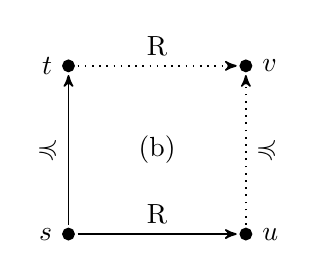
\begin{tikzpicture}[modal,node distance = 10mm]
        \node (c) {(b)};
        \node[point] (a) [above left=of c,label=left:$t$] {};
        \node[point] (b) [above right=of c,label=right:$v$] {};
        \node[point] (d) [below left=of c,label=left:$s$] {};
        \node[point] (e) [below right=of c,label=right:$u$] {};
        \path[->] (a) edge[dotted] node[above] {$\R$} (b);
        \path[->] (d) edge node[above] {$\R$} (e);
        \path[->] (d) edge node[left] {$\preccurlyeq$} (a);
        \path[->] (e) edge[dotted] node[right] {$\preccurlyeq$} (b);
    \end{tikzpicture}
    \hspace{1.5cm}
    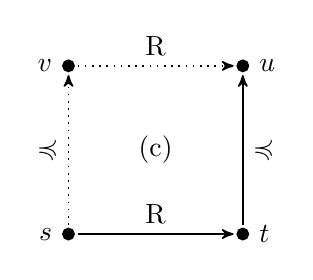
\begin{tikzpicture}[modal,node distance = 10mm]
        \node (c) {(c)};
        \node[point] (a) [above left=of c,label=left:$v$] {};
        \node[point] (b) [above right=of c,label=right:$u$] {};
        \node[point] (d) [below left=of c,label=left:$s$] {};
        \node[point] (e) [below right=of c,label=right:$t$] {};
        \path[->] (a) edge[dotted] node[above] {$\R$} (b);
        \path[->] (d) edge node[above] {$\R$} (e);
        \path[->] (d) edge[dotted] node[left] {$\preccurlyeq$} (a);
        \path[->] (e) edge node[right] {$\preccurlyeq$} (b);
    \end{tikzpicture}
    \caption{Frame Conditions on Bi-relational Kripke models}
    \label{fig:bframe}
\end{figure}

\begin{definition}\label[definition]{def:imodel}
    A \defn{hierarchical model} is a pair $\hmodel = \tuple{\Khm, \Hleq}$ where:
    % \begin{enumerate}
    %     \setlength{\itemsep}{0pt}
    %     \item $\Khm$ is a non-empty set of Kripke models;
    %     \item $\Hleq$ is a preorder on $\Khm$.
    % \end{enumerate}
    $\Khm$ is a non-empty set of Kripke models; and $\Hleq$ is a preorder on $\Khm$ such that for all $\kmodel_1,\kmodel_2\in\Khm$ with $\kmodel_1 \Hleq \kmodel_2$:
        (a) ${\Wkm[1] \subseteq \Wkm[2]}$;
        (b) ${\Rkm[1] \subseteq \Rkm[2]}$; and
        (c) for all $s \in \Wkm[1]$, $\Vkm[1](s) \subseteq \Vkm[2](w)$.
    % \begin{enumerate}[label=(\alph*)]
    %     \setlength{\itemsep}{0pt}
    %     \item ${\Wkm[1] \subseteq \Wkm[2]}$;
    %     \item ${\Rkm[1] \subseteq \Rkm[2]}$;
    %     \item for all $s \in \Wkm[1]$, $\Vkm[1](s) \subseteq \Vkm[2](w)$.
    % \end{enumerate}
    %%We use $\kmodels_{\hmodel}$, and $\preccurlyeq_{\hmodel}$, to indicate $\kmodels$, and $\preccurlyeq$, respectively.
\end{definition}

% \begin{proposition}
%     If $\bmodel$ is a hierarchical model, then, $\preccurlyeq_{\bmodel}$ is a partial order.
% \end{proposition}
% \begin{proof}
%     We only need to prove that $\preccurlyeq_{\bmodel}$ is antisymmetric, i.e., if $\kmodel_1 \preccurlyeq_{\bmodel} \kmodel_2$ and $\kmodel_2 \preccurlyeq_{\bmodel} \kmodel_1$, then, $\kmodel_1 = \kmodel_2$.
%     The result is immediate from conditions (a)--(c).
% \end{proof}

\begin{definition}\label[definition]{def:sat:imodel}
    Let $\hmodel$ be a hierarchical model, $\kmodel \in \Khm$, and $s \in \Wkm$.
    Moreover, let $A$ be a formula.
    The \defn{forcing relation} $\hforces {\pair \kmodel s} A$ is defined inductively as:
    \[\begin{array}{lcl}
        \hforces {\pair \kmodel s} \bot
            & \text{iff} & \text{false} \\
        \hforces {\pair \kmodel s} p
            & \text{iff} & p \in \Vkm(s) \\
        \hforces {\pair \kmodel s} {B \land C}
            & \text{iff} & \hforces {\pair \kmodel s} B \text{ and } \hforces {\pair \kmodel s} C \\
        \hforces {\pair \kmodel s} {B \lor C}
            & \text{iff} & \hforces {\pair \kmodel s} B \text{ or } \hforces {\pair \kmodel s} C \\
        \hforces {\pair \kmodel s} {B \to C}
            & \text{iff} & \text{for all } \kmodel' \in \Khm,~
                \text{if } \kmodel \Hleq \kmodel' \text{ and } \hforces {\pair {\kmodel'} s} B
                    \text{, then, } \hforces {\pair {\kmodel'} s} C \\
        \hforces {\pair \kmodel s} \Diamond B & \text{iff}
            & \text{exists } t \in \Wkm \text{ such that } s \Rkm t \text{ and } \hforces {\pair \kmodel t} B \\
        \hforces {\pair \kmodel s} \Box B & \text{iff}
            & \text{for all } \kmodel' \in \Khm,~
                \text{if } \kmodel \Hleq \kmodel' \text{, then, }
                    \text{for all } t \in \Wof{\kmodel'},
                        \text{ if } s \Rof{\kmodel'} t \text{, then, } \hforces {\pair {\kmodel'} t} B.
    \end{array}\]
    We use $\nhforces {\pair \kmodel s} A$ to indicate the negation of $\hforces {\pair \kmodel s} A$.
    Immediately, $\hforces {\pair \kmodel s} \lnot B$ iff for all $\kmodel' \in \Khm$, if $\kmodel \Hleq \kmodel'$, then, $\nhforces {\pair {\kmodel'} s} B$.
    % We write $\forces\hmodel A$ iff $\hforces{\pair \kmodel s} A$ for all $\kmodel\in\Khm$ and $s\in \Wkm$.
    % Finally, we write $\Vdash A$, and call $A$ a tautology, iff $\Vdash^{\hmodel} A$ for all hierarchical models $\hmodel$.\lutz{we can't define tautology twice!}
\end{definition}

The hierarchical semantics aligns closely with the standard semantic treatment of intuitionistic propositional and first-order logic, where models are organised into layers ordered by inclusion, reflecting the monotonic growth of information \cite{Troelstra1988}. This conceptual proximity is one of its main attractions. This same feature, however, also leads to a significant limitation: the hierarchical semantics fails to enjoy the finite model property. A classical counterexample, originating in the work of Ono and Suzuki~\cite{ono1988}, is the formula $\Box \neg \neg \varphi \to \neg \neg \Box \varphi$. This formula can be falsified only in infinite hierarchical models.

Alternative to the hierarchical semantics for $\IK$ is the bi-relational semantics. We introduce this alternative semantics next.

\begin{definition}\label[definition]{def:bmodel}
    A \defn{birelational Kripke model} is a cuadruple of the form $\bmodel = \tuple{\Wbm, \Fbm, \Rbm, \Vbm}$ where:
    % \begin{enumerate}
    %     \setlength{\itemsep}{0pt}
    %     \item $\Wbm$ is a non-empty set of \defn{worlds};
    %     \item $\Fbm$, the \defn{future relation},    is a preorder (reflexive and transitive) on $\Wbm$;
    %     \item $\Rbm$ is a binary \defn{accessibility relation} on $\Wbm$;
    %     \item $\Vbm\colon \props \to 2^{\Wbm}$ is a \defn{valuation function}.
    % \end{enumerate}
    $\tuple{\Wbm, \Rbm, \Vbm}$ is a Kripke model, and 
    $\Fbm$, the \defn{future relation}, is a preorder on $\Wbm$
    such that
%%    Bi-relational Kripke models further satisfy the following conditions:
    \begin{enumerate}[label=(\alph*)]
        \setlength{\itemsep}{0pt}
        \item for all $s,t\in\Wbm$, if $s \Fbm t$ and $p \in \Vbm(s)$, then, $p \in \Vbm(t)$.
        \item for all $s,t,u\in\Wbm$, if $s \Fbm t$ and $s \Rbm u$, then, there is $v \in \Wbm$ such that $t \Rbm v$ and $u \Fbm v$;
        \item for all $s,t,u\in\Wbm$, if $s \Rbm t$ and $t \Fbm u$, then, there is $v \in \Wbm$ such that $s \Fbm v$ and $v \Rbm u$;
    \end{enumerate}
    The condition (a) above is referred to as \emph{monotonicity of valuations}.
    The conditions (b) and (c) above, depicted in \Cref{fig:bframe}, are commutativity conditions on future and accessibility relations.
    The conditions (b) and (c) are discussed in \cite[p.~51]{simpson1994}, under the names (F1) and (F2), respectively.
    % By a \defn{pointed birelational Kripke model}, we mean a pair $\pair \bmodel s$ where $\bmodel$ is a birelational Kripke model and $s \in \Wbm$.
    % We often omit the parentheses and write simply $\npair \bmodel s$ when there is no ambiguity.
    % If $v$ in (a) and (b) is unique, $\bmodel$ is called \defn{universal}.
    % We write $\preccurlyeq^{\equiv}$ and $\R^{\equiv}$ for the equivalence closure of $\preccurlyeq$ and $\R$, respectively.\lutz{what does that mean?}
    % We call $\bmodel$ \defn{cartesian} iff whenever $s \preccurlyeq^{\equiv} t$ and $t \R^{\equiv} u$, then, $s = u$.\todo{add index}
    % We use $\W_{\bmodel}$, $\preccurlyeq_{\bmodel}$, $\R_{\bmodel}$, and $\V_{\bmodel}$, to indicate $\W$, $\preccurlyeq$, $\R$, and $\V$, respectively.\lutz{We omit the index $\bmsymb$ ...}
\end{definition}

\begin{definition}\label[definition]{def:bsat}
    Let $\bmodel$ be a bi-relational model, $s \in \W_{\bmodel}$, and $A$ be a formula.
    The \defn{forcing relation} $\bforces s A$ is defined inductively as:
    \[\begin{array}{lcl}
            \bforces s \bot & \text{iff} & \text{false} \\
            \bforces s p & \text{iff} & p \in \V_{\bmodel}(s) \\
            %\bforces s \lnot B & \text{iff} & \text{for all } s \preccurlyeq_{\bmodel} t,~ \bmodel, t \nVdash B \\
            \bforces s {B \land C} & \text{iff} & \bforces s B \text{ and } \bforces s C \\
            \bforces s {B \lor C} & \text{iff} & \bforces s B \text{ or } \bforces s C \\
            \bforces s {B \to C} & \text{iff} & \text{for all } t \in \Wbm, \text{ if } s \Fbm t \text{ and } \bforces t B, \text{ then, } \bforces t C \\
            \bforces s {\Diamond B} & \text{iff} & \text{exists } s \in \Wbm \text{ such that } s \Rbm t \text{ and } \bforces t B \\
            \bforces s {\Box B} & \text{iff} & \text{for all } t,u \in \Wbm, \text{ if } s \Fbm t \text{ and } t \Rbm u, \text{ then, } \bforces u B.
    \end{array}\]
    We use $\nbforces s A$ to indicate the negation of $\bforces s A$.
    Immediately, $\bforces s \lnot B$ iff for all $t \in \Wbm$, if $s \Fbm t$, then, $\nbforces t B$.
    %We write $\forces \bmodel A$ iff $\bforces s A$ for all $s \in \Wbm$.
    % Moreover, we write $\sforce A$, and call $A$ a \defn{tautology}, iff $\bmodel \Vdash A$ for all bi-relational Kripke models $\bmodel$.
\end{definition}

We are now in position to comment on two key features of the bi-relational semantics for intuitionistic modal logic.
First, the clauses for $\Diamond$ and $\Box$ in \Cref{def:bsat} closely parallel those for the hierarchical semantics, and so for the existential and universal quantifiers in intuitionistic predicate logic~\cite{Troelstra1988}. This parallel reflects the constructive nature of the logic. Second,    conditions (b) and (c) in \Cref{def:bmodel} are traced back to the work of Plotkin in~\cite{PlotkinS86}, where they play a foundational role. Formally, condition (b) ensures the monotonicity of $\Diamond$: if $\bforces s {\Diamond A}$ and $s \Fbm t$, then $\bforces t {\Diamond A}$. In turn, condition (c) is motivated by the intuition that the formula $\lnot \Diamond A \to \Box \lnot A$ should hold---and by the fact that this implication fails if the condition is omitted.
While condition (b) can easily be regarded as natural, condition (c) is more debatable. This is also mentioned in~\cite{PlotkinS86,simpson1994}, where the authors themselves express greater confidence in the necessity of (b), acknowledging that (c) may be less well-justified.
In any case, condition (c) is nowadays accepted as inherent in a bi-relational model.

The following two propositions indicate the close semantic correspondence between the hierarchical and bi-relational models.

\begin{proposition}[{\cite[Lemma~8.1.2]{simpson1994}}]\label[proposition]{prop:hs2bks}
    Let $\hmodel$ be a hierarchical model.
    Define $\bmofhm = \tuple{\W, \Fsymb, \R, \V}$ where:
    \begin{enumerate}
        \setlength{\itemsep}{0pt}
        \item $\W = \setof{\pair\kmodel s}{ \kmodel \in \Khm \text{ and } s \in \Wkm}$;
        \item ${\Fsymb} = \setof{ (\pair{\kmodel_1}s, \pair{\kmodel_2} s) }{ \kmodel_1 \Hleq\kmodel_2 \text{ and } s\in    \Wkm[1]}$;
        \item $\R    = \setof{ (\pair{\kmodel}{s}, \pair{\kmodel}{t}) }{ \kmodel\in \Khm \text{ and } s \Rkm t}$;
        \item %$\V_{\hmodel}: \props \to 2^{\S_{\hmodel}}$ is s.t.\
            for all ${\pair \kmodel s} \in \W$, $\V(\npair \kmodel s) = \Vkm(s)$.
    \end{enumerate}
    It follows that:
        (a) $\bmofhm$ is a birelational Kripke model; and
        (b) for all formulas $A$, it follows that $\hforces{\pair\kmodel s} A$ ~iff~ $\xforces{\bmofhm}{\pair\kmodel s} A$.
    % \begin{enumerate}[label=(\alph*)]
    %     \setlength{\itemsep}{0pt}
    %     \item $\bmofhm$ is a birelational Kripke model;
    %     \item $\hforces{\pair\kmodel s} A$ ~iff~ $\xforces{\bmofhm}{\pair\kmodel s} A$; and
    %     % \item if $\hmodel$ is finite, then, $\bmodel_{\hmodel}$ is finite.
    % \end{enumerate}
\end{proposition}

\begin{proposition}\label[proposition]{prop:iml}
    Let $A$ be any formula.
    The following are equivalent:
    \begin{enumerate}[label=(\alph*)]
        \setlength{\itemsep}{0pt}
        \item for all hierarchical models $\hmodel$, $\kmodel \in \Khm$, and $s \in \Wkm$, it follows that $\hforces{\pair \kmodel s}{A}$;
        \item for all bi-relational models $\bmodel$, and $s \in \Wbm$, it follows that $\bforces{s}{A}$.
    \end{enumerate}
\end{proposition}

% In \cite[$\S$~8.1.2]{brauner11}, it is claimed that, in general, bi-relational Kripke models cannot be translated into hierarchical models.
% The stated reason is that there are more bi-relational Kripke models than intuitionistic modal models, though no formal justification for this claim is provided.
% At the same time, in \cite[p.~152]{simpson1994}, it is shown that cartesian bi-relational Kripke models can be translated into hierarchical models in a semantic preserving way.
% \valentin{When we started to look into this problem Carlos messaged Torben about the claim he makes in his book. \lutz{what claim?} He replied, but did not provide a good justification for what he says. From the result in Simpson's PhD thesis, I think it should be clear that the translation from cartesian bi-relational Kripke models to hierarchical models cannot preserve finiteness, or cartesian bi-relational Kripke models cannot be used to characterize $\IK$.}\lutz{I think finiteness is easily preserved. but cartesian models are too restriced to have the FMP}

The result in~\Cref{prop:hs2bks} establishes that every hierarchical model can be translated into a bi-relational Kripke model in a truth-preserving way. In turn, the result in \Cref{prop:iml} establishes that the two frameworks validate the same formulas. As pointed out in \cite{simpson1994}, the latter result is surprising given the structural different between the frameworks. At the same time, the model-theoretic behaviour of the two frameworks differs in a crucial respect. Bi-relational models enjoy the finite model property, whereas hierarchical models do not. This asymmetry provides a clear indication that, although hierarchical models can be faithfully encoded into bi-relational ones, the converse translation cannot in general be done in finiteness-preserving way. In this sense, the bi-relational semantics offers a strictly more robust model-theoretic setting, even though both frameworks validate the same intuitionistic modal formulas.

%\section{A Wrinkle in Time}

\section{A New Semantics for \IML}

In this section, we introduce a new kind of model for interpreting formulas of $\IML$.
These new models, called \emph{weaved models}, are designed as a generalization of the hierarchical perspective on intuitionistic modal logic with the aim of making this model more explicit. Concretely, weaved models reflect the idea behind hierarchical models of interpreting formulas on a collection of related Kripke models organized in a meaningful way.
What makes weaved models particularly useful is that, they are compatible with important metatheoretic results, such as the finite model property. In this way, weaved models combine the conceptual clarity of hierarchical models with the formal strengths of birelational Kripke models.

\subsection{Weaved models}

We begin with a technical preliminary definition.

\begin{definition}\label[definition]{def:simulation}
        A \defn{simulation} from a Kripke model $\kmodel_1$ to a Kripke model $\kmodel_2$ is a non-empty binary relation $\Sim \subseteq (\Wkm[1] \times \Wkm[2])$ such that, for all $s_1 \in \Wkm[1]$ and $s_2 \in \Wkm[2]$, if $s_1 \Sim s_2$, then:
        \begin{description}
                \setlength{\itemsep}{0pt}
                \item[\textnormal{(add)}] if $p \in \Vkm[1](s_1)$, then, $p \in \Vkm[2](s_2)$;
                \item[\textnormal{(see)}] for all $s_3 \in \Wkm[1]$, if $s_1 \Rkm[1] s_3$, then, there is $s_4 \in \Wkm[2]$ such that $s_2 \Rkm[2] s_4$ and $s_3 \Sim s_4$.
        \end{description}
        The relation $\Sim$ is a \defn{seesaw simulation} from $\kmodel_1$ to $\kmodel_2$,
        denoted as $\Sim\colon\kmodel_1\fsim\kmodel_2$, if it is both: a simulation from $\kmodel_1$ to    $\kmodel_2$, and a simulation from $\ikmodel_1$ to    $\ikmodel_2$.
        Here, $\ikmodel_{i} = \tuple{\Qkm[i],\iRkm[i],\Vkm[i]}$ is the \defn{inverse} of $\kmodel[i]$ for $i \in \set{1,2}$.
\end{definition}

\begin{proposition}
        The following two conditions are equivalent:
        \begin{enumerate}[leftmargin=\parindent]
                \item $\Sim$ is a seesaw simulation from $\kmodel_1$ to $\kmodel_2$.
                \item $\Sim$ is a simulation such that: (saw) for all $s_3 \in \Wkm[1]$, if $s_3 \Rkm[1] s_1$, then, exists $s_4 \in \Wkm[2]$ such that $s_4 \Rkm[2] s_2$ and $s_3 \Sim s_4$.
        \end{enumerate}
        \lutz{is there some $s_1\Sim s_2$ missing in (2)?}
\end{proposition}

\begin{definition}\label[definition]{def:simulation}
	A \defn{forward and backwards simulation} (from now on, a simulation for simplicity) from a Kripke model $\kmodel_1$ to a Kripke model $\kmodel_2$ (notation: $\Sim\colon\kmodel_1\fsim\kmodel_2$) is a non-empty binary relation $\Sim \subseteq (\Wkm[1] \times \Wkm[2])$ such that, for all $s_1 \in \Wkm[1]$ and $s_2 \in \Wkm[2]$, if $s_1 \Sim s_2$, then:
	\begin{description}
		\setlength{\itemsep}{0pt}
		\item[\textnormal{(add)}] if $p \in \Vkm[1](s_1)$, then, $p \in \Vkm[2](s_2)$;
		\item[\textnormal{(forth)}] for all $s_3 \in \Wkm[1]$, if $s_1 \Rkm[1] s_3$, then, there is $s_4 \in \Wkm[2]$ such that $s_2 \Rkm[2] s_4$ and $s_3 \Sim s_4$;
		\item[\textnormal{(back)}] for all $s_3 \in \Wkm[1]$, if $s_3 \Rkm[1] s_1$, then, there is $s_4 \in \Wkm[2]$ such that $s_4 \Rkm[2] s_2$ and $s_3 \Sim s_4$.
	\end{description}
\lutz{what is this def doing here? isn't this the same as 3.1?}
\end{definition}

\begin{proposition}
        For every Kripke model $\kmodel$, the identity (or diagonal) relation $\Delta_{\Qkm}=\setof{(q,q)}{q\in\Qkm}$ is a seesaw simulation $\id_{\kmodel}\colon\kmodel \fsim \kmodel$. Moreover, the composition $\Sim\relcomp\Tim\colon \kmodel_1 \fsim \kmodel_3$ of seesaw simulations $\Sim\colon\kmodel_1 \fsim \kmodel_2$ and ${\Tim\colon\kmodel_2 \fsim \kmodel_3}$ is a seesaw simulation.
\end{proposition}

\todo{decide if we need to define inverse and composition of relations in the beginning}

We have adopted simulations as the foundational relational tool for connecting individual Kripke models. In fact, seesaw simulations turn out to be the right kind of simulation for organizing these models into the layered architecture characteristic of weaved models. Intuitively, the conditions (see) and (saw) that characterize a seesaw simulation correspond closely to conditions (b) and (c) in the definition of bi-relational models. The formal definition of weaved models will make clear how seesaw simulations are used to assemble individual Kripke models into a cohesive whole, while preserving a hierarchical organization. This definition also makes immediate how weaved models reflects the same underlying intuition as hierarchical models, but achieves it in a more flexible way.

\begin{definition}\label[definition]{def:wmodel:simulation}
    A \defn{weaved model} is a pair $\wmodel = \tuple{\Kwm, \Swm}$ where:
    \begin{enumerate}[leftmargin=\parindent]
        \setlength{\itemsep}{0pt}
        \item $\Kwm$ is a non-empty set of Kripke models;
        % \item $\Fbm$ is a preorder on $\kmodels$;
        \item $\Swm$ is a set of seesaw simulations on $\Kwm$ closed under identities and composition.
    \end{enumerate}
%%    We use $\kmodels_{\wmodel}$, and $\G_{\wmodel}$, to indicate $\kmodels$, and $\G$, respectively.
    For any weaved model $\wmodel$, we define the set
    \begin{equation}
        \Qwm=\setof{\pair{\kmodel}q}{\kmodel\in\Kwm\mbox{ and } q\in\Qkm}
    \end{equation}
    and on this set we define the binary relation
    \begin{equation}
        \Fwm=\setof{(\pair\kmodel q,\pair{\kmodel'}{q'})}{\mbox{there is ${\Sim\colon\kmodel\fsim\kmodel'} \in \Swm$ with $q\Sim q'$}}.
    \end{equation}
\end{definition}

\begin{proposition}\label[proposition]{prop:preorder:wmodel}
    Let $\wmodel$ be a weaved model. \!Then, $\Fwm$ is a preorder~on~$\Qwm$.
\end{proposition}

\Cref{prop:preorder:wmodel} shows that, although weaved models do not specify a future relation explicitly, such a relation can still be recovered from their internal organization via seesaw simulations. This stands in contrast to bi-relational and hierarchical models, where the future relation is built directly into their definition. This result highlights a key feature of weaved models: they preserve the essential idea of a hierarchical arrangement of Kripke models, but achieve this using simulations instead of rigid relational constraints of hierarchical models. This approach allows for greater flexibility while still supporting the logical properties we expect in an intuitionistic modal setting.

\begin{definition}\label[definition]{def:sat:wmodel:simulation}
    Let $\wmodel$ be a weaved model, and ${\pair \kmodel s} \in \Qwm$.
    Moreover, let $A$ be a formula.
    The \defn{forcing relation} $\wforces {\pair \kmodel s} A$ is defined inductively as:
%%    The relation $\wforces {\pair \kmodel s} A$ is defined recursively as:
    \[\begin{array}{lcl}
        \wforces {\pair \kmodel s} \bot
            & \text{iff} & \text{false} \\
        \wforces {\pair \kmodel s} p
            & \text{iff} & p \in \Vkm(s) \\
        \wforces {\pair \kmodel s} {B \land C}
            & \text{iff} & \wforces {\pair \kmodel s} B \text{ and } \wforces {\pair \kmodel s} C \\
        \wforces {\pair \kmodel s} {B \lor C}
            & \text{iff} & \wforces {\pair \kmodel s} B \text{ or } \wforces {\pair \kmodel s} C \\
        \wforces {\pair \kmodel s} {B \to C}
            & \text{iff} & \text{for all } {\pair {\kmodel'} t} \in \Qwm, \\
            && \quad \text{if } {\pair \kmodel s} \Fwm {\pair {\kmodel'} t} \text{, then, } \\
            && \qquad \text{if } \wforces {\pair {\kmodel'} t} B \text{, then, } \wforces {\pair {\kmodel'} t} C \\
        \wforces {\pair \kmodel s} \Diamond B & \text{iff}
            & \text{exists } t \in \Wkm \text{ such that } s \Rkm t \text{ and } \wforces {\pair \kmodel t} B \\
        \wforces {\pair \kmodel s} \Box B & \text{iff}
            & \text{for all } {\pair {\kmodel'} t} \in \Qwm, \\
            && \quad \text{if } {\pair \kmodel s} \Fwm {\pair {\kmodel'} t} \text{, then, } \\
            && \qquad \text{for all } u \in \Wof{\kmodel'}, \text{ if } t \Rof{\kmodel'} u \text{, then, } \wforces {\pair {\kmodel'} u} B.
    \end{array}\]
    We use $\nwforces {\pair \kmodel s} A$ to indicate the negation of $\wforces {\pair \kmodel s} A$.
    Immediately, $\nwforces {\pair \kmodel s} \bot$, and $\wforces {\pair \kmodel s} \lnot B$ iff for all $\kmodel' \in \Khm$, if $\kmodel \Fwm \kmodel'$, then, $\nwforces {\pair {\kmodel'} s} B$.
\end{definition}

With the forcing relation for weaved models in place, we turn our attention to commenting on some of its features as a semantic framework for intuitionistic modal logic.
The most basic of these features is monotonicity, made precise in \Cref{prop:monotonicity:ws} below.

\begin{proposition}[Monotonicity]\label[proposition]{prop:monotonicity:ws}
    Let $\wmodel$ be a weaved model, and $A$ be a formula.
    For all ${\pair {\kmodel_1} s}, {\pair {\kmodel_2} t} \in \Qwm$, if $\wforces{\pair {\kmodel_1} s}{A}$ and ${\pair {\kmodel_1} s} \Fwm {\pair {\kmodel_2} t}$, then, $\wforces {\pair {\kmodel_2} t} A$.
\end{proposition}
\begin{proof}
    %Suppose $\wforces{\pair \kmodel s}{A}$ and ${\pair \kmodel s} \Fwm {\pair {\kmodel'} t}$.
    We prove the result by a case analysis and induction on~$A$.

    \medskip
    \noindent
    For formulas of the form $p$, $B \to C$, and $\Box B$, the result follows from the fact that monotonicity is built into the definition of the forcing relation for weaved models.
    We illustrate the case of $\Box B$ as representative of this fact.
    Suppose that (1) $\wforces {\pair {\kmodel_1} s} \Box B$, and ${\pair {\kmodel_1} s} \Fwm {\pair {\kmodel_2} t}$ for an arbitrary ${{\pair {\kmodel_2} t} \in \Qwm}$.
    We need to establish $\wforces {\pair {\kmodel_2} t} \Box B$.
    We proceed by contradiction.
    Let ${\nwforces {\pair {\kmodel_2} t} \Box B}$.
    There are ${\pair {\kmodel_3} u} \in \Qwm$ and $v \in \Wkm[3]$ s.t.\ ${\pair {\kmodel_2} t} \Fwm {\pair {\kmodel_3} u}$, $u \Rkm[3] v$, and $\nwforces {\pair {\kmodel_3} v} B$.
    From the transitivity of $\Fwm$, ${\pair {\kmodel_1} s} \Fwm {\pair {\kmodel_3} u}$.
    But this fact contradicts (1).
    Therefore, $\wforces {\pair {\kmodel_2} t} \Box B$.

    \medskip
    \noindent
    The cases of conjunctions $B \land C$, disjunctions $B \lor C$, and diamonds $\Diamond B$ are proven by induction.
    The base cases are immediate.
    The inductive hypothesis assumes monotonicity holds for an arbitrary formula.
    We illustrate the case of $\Diamond B$ as representative of the reasoning involved in the inductive step.
    Suppose (2) ${\wforces {\pair {\kmodel_1} s} \Diamond B}$, and (3) ${\pair {\kmodel_1} s} \Fwm {\pair {\kmodel_2} t}$ for an arbitrary ${\pair {\kmodel_2} t} \in \Qwm$.
    We need to establish $\wforces {\pair {\kmodel_2} t} \Diamond B$.
    From (2), we know there is $u \in \Qkm[1]$ such that $s \Rkm[1] u$ and $\wforces {\pair {\kmodel_1} u} B$.
    From (3), we know there is a seesaw simulation $\Sim \colon {\kmodel_1 \fsim \kmodel_2} \in \Swm$ such that $s \Sim u$.
    The (see) condition ensures there is $v \in \Wkm[2]$ such that (4) $t \Rkm[2] v$ and $u \Sim v$. This guarantees that ${\pair{\kmodel_1}{u}} \Fwm {\pair{\kmodel_2}{v}}$. By the inductive hypothesis, we have $\wforces{\pair{\kmodel_2}{v}} B$. Combining this last step with (4), we conclude that $\wforces{\pair{\kmodel_2}{t}} \Diamond B$.
\end{proof}

The use of the (see) condition in the proof of \Cref{prop:monotonicity:ws} highlights its essential role in the definition of seesaw.
Intuitively, the condition serves the same purpose in weaved models as condition (b) in \Cref{def:bmodel} does for bi-relational models, and condition (b) in \Cref{def:imodel} does for hierarchical models. In each case, these conditions ensure that the modal accessibility relation behaves in a way that preserves the constructive, monotonic nature of the logic across related worlds.
The following example illustrates the role played by (saw) in the definition of a seesaw simulation.

\begin{example}\label[example]{ex:plotkin}
    \def\pwmodel{\mathfrak{S}}
    The model in \Cref{fig:weaved:plotkin} illustrates what can go wrong if we restrict ourselves to simulations instead of seesaw simulations in a weaved model.
    Formally, this model is the pair $\pwmodel = \tuple{\set{\kmodel_1, \kmodel_2}, \set{\id_{\kmodel_1}, \id_{\kmodel_2}, \Sim}}$, where:
        \[
            \kmodel_1 = \tuple{\set{s, t}, \set{(s, t)}, \Vkm[1]}
            \quad \text{and} \quad
            \kmodel_2 = \tuple{\set{u,v,w}, \set{(u, v)}, \Vkm[2]}
        \]
    are Kripke models with valuations $\Vkm[1](s) = \Vkm[1](t) = \Vkm[2](u) = \Vkm[2](v) = \emptyset$ and $\Vkm[2](w) = \set{p}$.
    The relation $\Sim = \set{(s, u), (t, v)}$ is a (total) simulation from $\kmodel_1$ to $\kmodel_2$ that is not a seesaw simulation.
    If we keep the semantic clauses from \Cref{def:sat:wmodel:simulation}, it is easy to verify that $\xforces{\pwmodel}{\pair{\kmodel_1}{s}}{\lnot \Diamond p}$ holds, while $\xforces{\pwmodel}{\pair{\kmodel_1}{s}}{\Box \lnot p}$ fails. Consequently, we obtain $\nxforces{\pwmodel}{\pair{\kmodel_1}{s}}{\lnot \Diamond p \to \Box \lnot p}$.
    This outcome conflicts with the intuition that the formula $\lnot \Diamond A \to \Box \lnot A$ should hold in an intuitionistic modal setting. Seesaw simulations---particularly the (saw) property---rule out exactly these kinds of counterexamples.
\end{example}

\begin{figure}[!t]
    \centering
    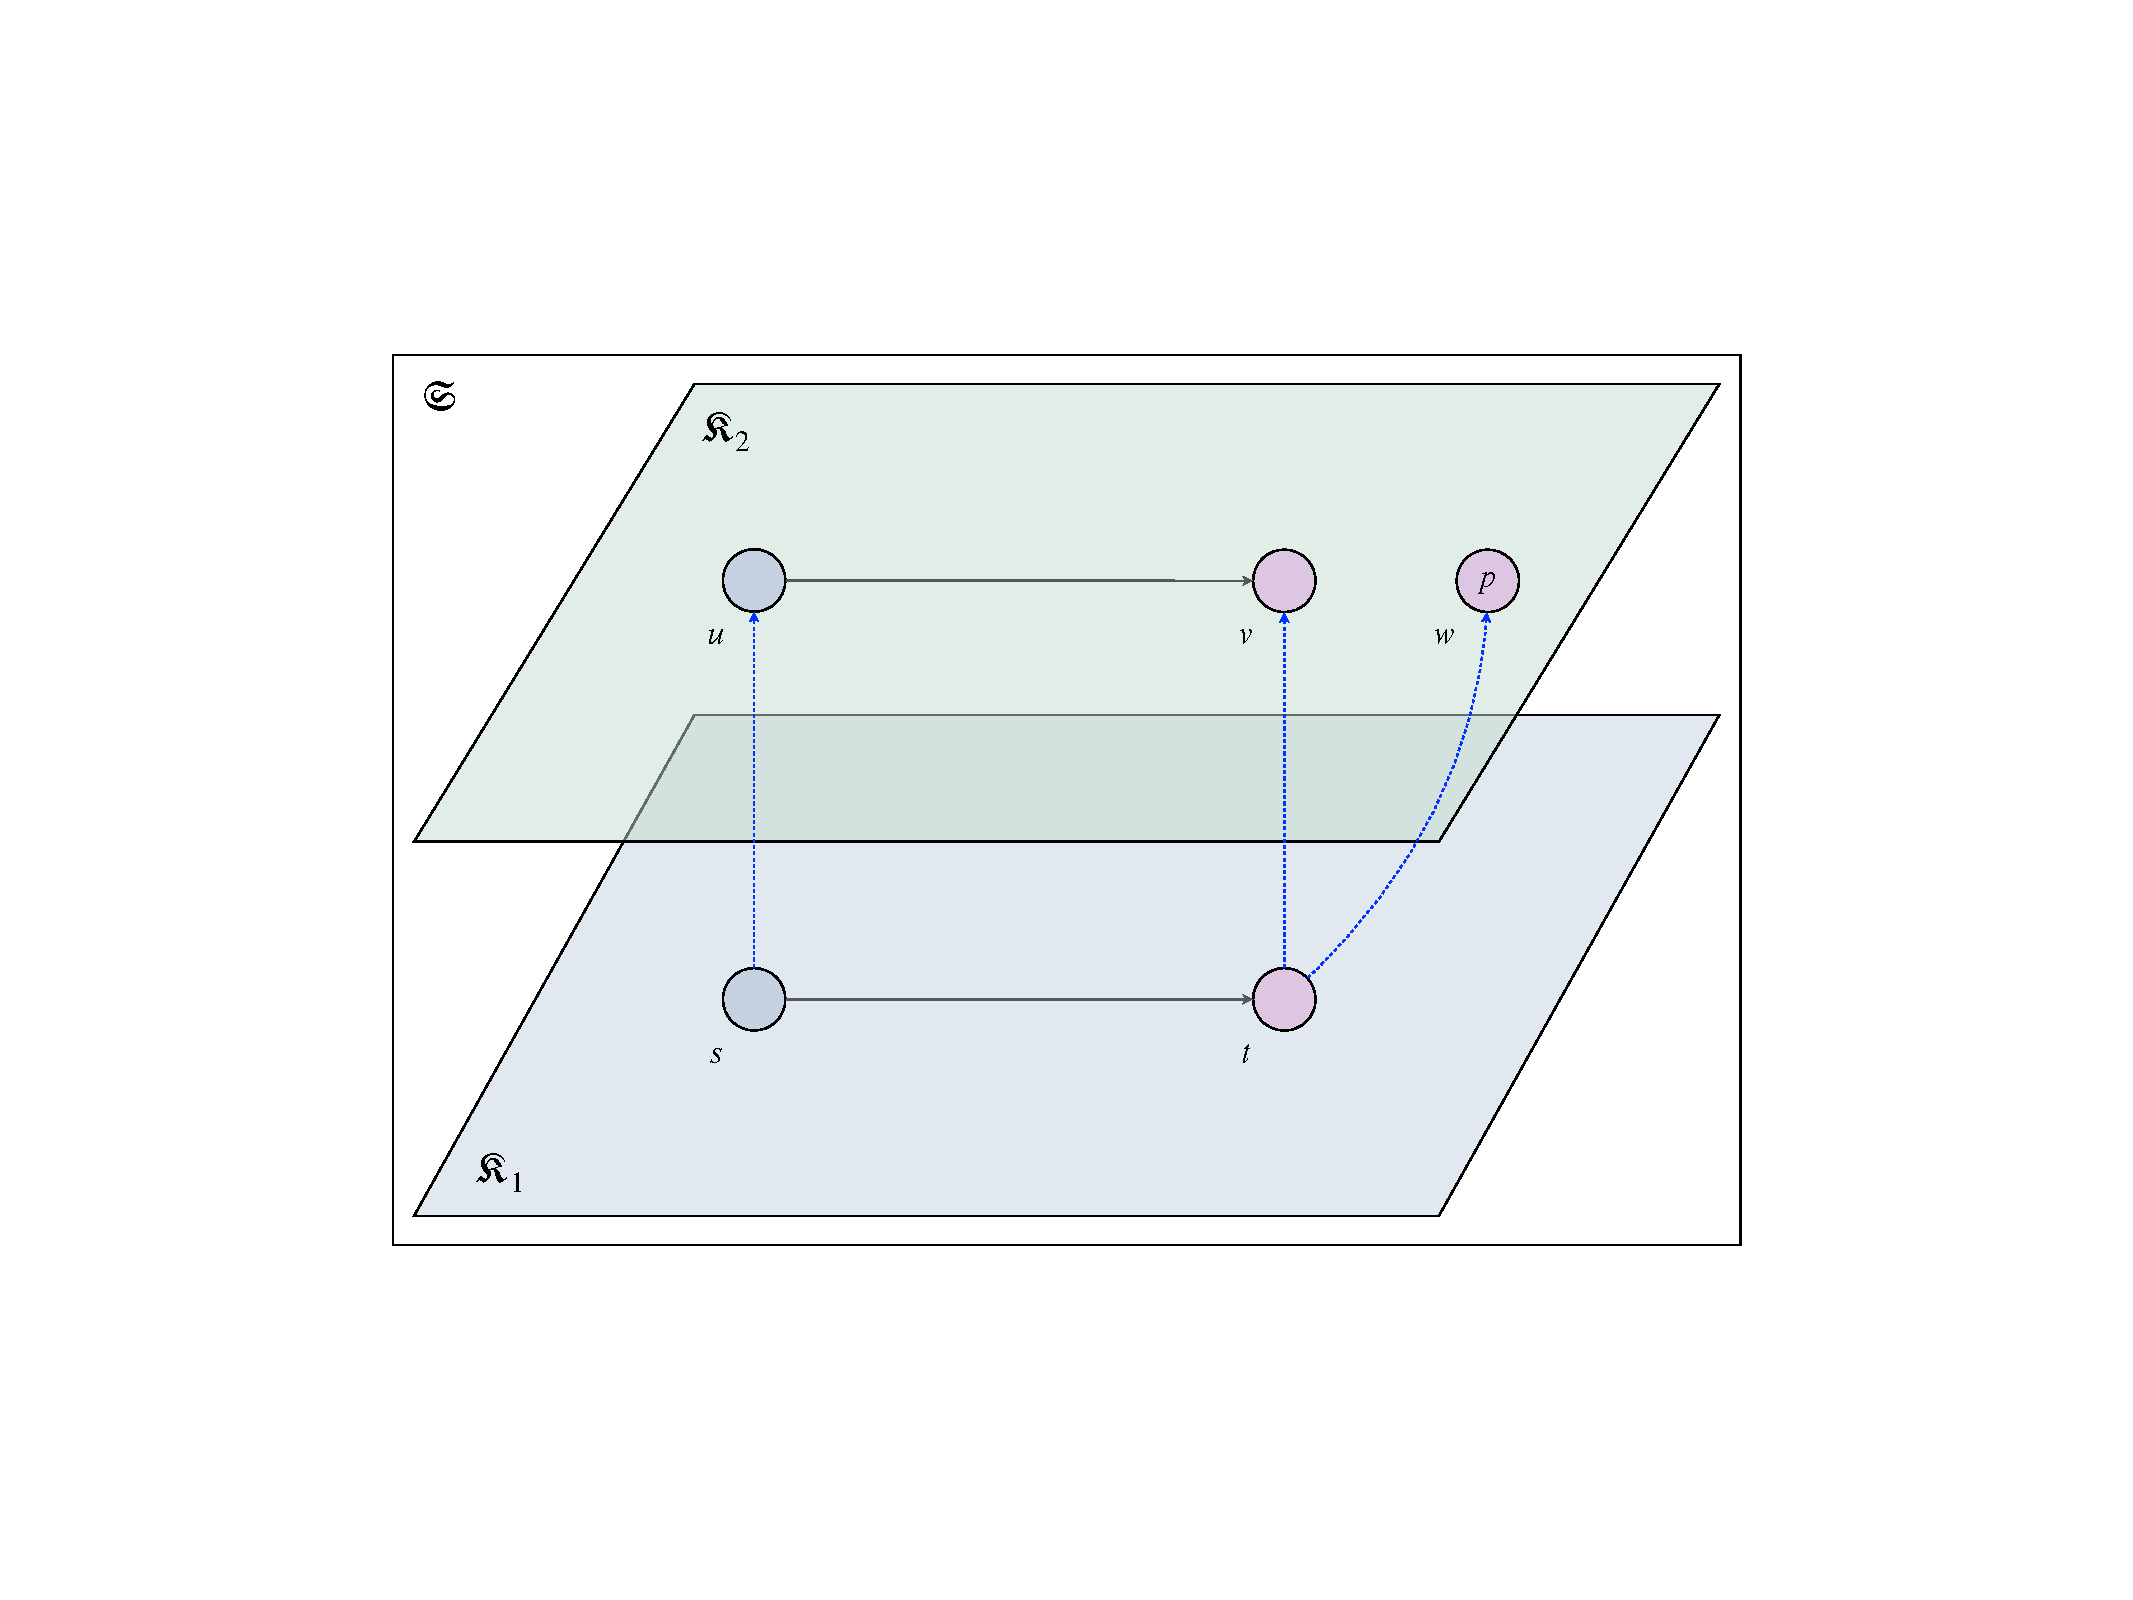
\includegraphics[height=4.9cm]{figures/plotkin.pdf}
    \caption{The Importance of (saw) in Seesaw Simulations}
    \label{fig:weaved:plotkin}
\end{figure}

The next result further elaborates on the point made in \Cref{ex:plotkin}.

\begin{proposition}
    Let $\wmodel$ be a weaved model.
    Then, for all ${\pair {\kmodel_1} s} \in \Qwm$, $\wforces{\pair {\kmodel_1} s}{\lnot \Diamond A \to \Box \lnot A}$.
\end{proposition}
\begin{proof}
    The proof is by contradiction.
    Let $\nwforces{\pair {\kmodel_1} s}{\lnot \Diamond A \to \Box \lnot A}$.
    There is ${\pair {\kmodel_2} t} \in \Qwm$ such that:
        (1) ${\pair {\kmodel_1} s} \Fwm {\pair {\kmodel_2} t}$,
        (2) $\wforces{\pair {\kmodel_2} t}{\lnot \Diamond A}$, and
        (3) $\nwforces{\pair {\kmodel_2} t}{\Box \lnot A}$.
    % From (2),
    %     for all ${\pair {\kmodel_3} u} \in \Qwm$,
    %         if ${\pair {\kmodel_2} t} \Fwm {\pair {\kmodel_3} u}$, then,
    %             $\nwforces{\pair {\kmodel_3} u}{\Diamond A}$.
    From (3),
        there are ${\pair {\kmodel_3} u} \in \Qwm$ and ${v \in \Wkm[3]}$ such that
            ${\pair {\kmodel_2} t} \Fwm {\pair {\kmodel_3} u}$,
            $u \Rkm[3] v$, and
            $\nwforces{\pair {\kmodel_3} v}{\lnot A}$.
    This implies there is ${\pair {\kmodel_4} w} \in \Qwm$ such that
        (4) ${\pair {\kmodel_3} v} \Fwm {\pair {\kmodel_4} w}$, and
        $\wforces{\pair {\kmodel_4} w}{A}$.
    From (4), there is $\Sim \colon \kmodel_3 \fsim \kmodel_4$ such that $v \Sim w$.
    By the (saw) property, there is $w \in \Wkm[4]$ such that $v \Sim x$ and $x \Rkm[4] w$.
    And so, $\wforces{\pair {\kmodel_4} x}{\Diamond A}$.
    But this fact contradicts (2), as we have
        ${\pair {\kmodel_2} t} \Fwm {\pair {\kmodel_4} x}$, and
        $\wforces{\pair {\kmodel_4} x}{\Diamond A}$.
\end{proof}

We are now in a position to reflect on weaved models from a more conceptual standpoint. To guide this discussion, we follow the perspective outlined in \cite{simpson1994}, where it is noted that, within the Kripkean framework for intuitionistic logic, atomic facts are expected to persist into the future. That is, if an atomic proposition holds at a given world, it must continue to hold at all future worlds.

This principle can be extended beyond propositional atoms to the accessibility relation itself. In particular, if we treat the statement \emph{a world sees another world} as a kind of structural atomic fact, then the accessibility relation becomes subject to the same persistence requirement. This view provides a conceptual foundation for condition (b) in \Cref{def:bmodel} for bi-relational models, condition (b) in \Cref{def:imodel} for hierarchical models, and the (see) condition in seesaw simulations for weaved models.
The dual perspective, i.e., treating \emph{a world is seen by another} also as a kind of structural atomic fact, supports condition (c) in both \Cref{def:bmodel} and \Cref{def:imodel}, and the (saw) property for seesaw simulations.

In a hierarchical or layered setting, the idea of persistence can be extended even further. If a world $w$ exists at one point in the hierarchy, then it is natural to expect that $w$ continues to exist in the future, possibly with additional information. This intuition is captured explicitly as condition (a) in \Cref{def:imodel}.
For weaved models, the situation is more nuanced. The persistence of worlds is not built into the model itself but is instead governed by the properties of the seesaw simulations. Totality of the simulation relation would ensure the persistence of all worlds, but since totality plays no essential technical role in our results, we have chosen to set it aside. In this respect, the kind of persistence of worlds needed in weaved models is supported by the combination of (see) and (saw).
That said, while (see) and (saw) collectively achieve the required semantic effects, we acknowledge that they lack the broader conceptual justification that totality enjoys within the Kripkean paradigm.

\lutz{this discussion might be great for a philopsophy journal, but it will kill the paper for LICS.}

\subsection{From Weaved to Bi-relational and hierarchical models (and Back)}

To better understand the role of weaved models within intuitionistic modal logic, we examine how they relate to bi-relational and hierarchical models. Precisely, we show how weaved models can be seen as a generalization encompassing both frameworks. This comparison not only clarifies the conceptual foundations of weaved models but also highlights their flexibility in capturing layered modal behavior.

% Let $\hmodel$ be a hierarchical model and $\kmodel_1,\kmodel_2\in\Khm$ with $\kmodel_1\Fhm\kmodel_2$. We define the relation $\Sof{\kmodel_1,\kmodel_2}=\Delta_{\Qkm[1]}\subseteq\Qkm[1]\times\Qkm[1]\subseteq\Qkm[1]\times\Qkm[2]$. By Proposition..... this is a seesaw simulation $\Sof{\kmodel_1,\kmodel_2}\colon\kmodel_1\fsim\kmodel_2$.

\begin{proposition}\label{prop:hs2ws}
    Let $\hmodel$ be a hierarchical model.
    % Define the pair $\wmofhm=\tuple{\Kof{\wmofhm},\Sof{\wmofhm}}$ where $\Kof{\wmofhm}=\Khm$ and $\Sof{\wmofhm}=\setof{\Sof{\kmodel_1,\kmodel_2}}{\kmodel_1\Fhm\kmodel_2}$.
    Then, the pair
        \[
            \wmofhm = \tuple{\Khm,\setof{\Wkm[1] \isym \Wkm[2]}{\kmodel_1 \Hleq \kmodel_2}}
            \footnote{For $X \subseteq Y$, $X \isym Y$ indicates the inclusion map, i.e., the mapping of $x \in X$ to $x \in Y$. \lutz{don't make this a footnote. that should be in the main text}}
        \] 
    satisfies the following properties:
    %% It follows that:
    \begin{enumerate}[leftmargin=\parindent]
        \setlength{\itemsep}{0pt}
        \item $\wmofhm$ is a weaved model.
        \item $\hmodel$ is finite implies $\wmofhm$ is finite.
        \item $\hforces{\pair\kmodel s}A$ ~iff~ $\xforces{\wmofhm}{\pair\kmodel s} A$.
    \end{enumerate}
\end{proposition}
\begin{proof}
    Let $\wmofhm = \tuple{\Khm, \Swm}$.
    For item (1), it suffices to show that all inclusion maps ${\Wkm[1] \isym \Wkm[2]} \in \Swm$ are seesaw simulations, and that $\Swm$ is closed by identities and composition. But this follows immediately from the definition.
    Item (2) is similarly straightforward.
    For item (3), note that the forcing relation for weaved models aligns with that of hierarchical models, if all seesaw simulations are total and functional relations. If in addition the seesaw relations are inclusion maps, the semantics behaves identically across both settings.
\end{proof}

In brief, \Cref{prop:hs2bks} reveals that hierarchical models can be viewed as a special case of weaved models---those in which the connecting seesaw simulations are inclusion maps. Conceptually, this further highlights how weaved models capture the same foundational idea of layering Kripke models over time, but with greater flexibility: instead of requiring rigid inclusions, they allow more general relational connections while preserving the essential intuitionistic modal behavior.

\begin{proposition}\label[proposition]{prop:ws2bks}
    %% Let $\wmodel$ be a weaved model.
    %% Also, let $\bmodel_{\wmodel} = \tuple{\W, {\preccurlyeq}, \R, \V}$ be s.t.:
    %% \begin{enumerate}[leftmargin=\parindent]
    %%     \setlength{\itemsep}{0pt}
    %%     \item $\W = \setof{(\kmodel, s)}{ \kmodel \in \kmodels_{\wmodel} \text{ and } s \in \W_{\kmodel}}$;
    %%     \item ${\preccurlyeq} = \setof{ (\bb{s}, \bb{t}) }{ {f:{\bb{s}_1 \to \bb{t}_1} \in \Swm} \text{ and } {f(\bb{s}_2) = \bb{t}_2}}$;
    %%     \item $\R = \setof{ (\bb{s}, \bb{t}) }{ \set{\bb{s}_1, \bb{t}_1} \subseteq \kmodels_{\wmodel} \text{ and } {\bb{s}_1 = \bb{t}_1} \text{ and } {\bb{s}_2 \R_{\bb{s}_1} \bb{t}_2}}$;
    %%     \item %$\V_{\wmodel}: \props \to 2^{\S_{\wmodel}}$ is s.t.\
    %%         for all $\bb{s} \in \W$, $\V(s) = \V_{\bb{s}_1}(\bb{s}_2)$.
    %% \end{enumerate}
    %% It follows that:
    %% \begin{enumerate}[label=(\alph*)]
    %%     \setlength{\itemsep}{0pt}
    %%     \item $\bmodel_{\wmodel}$ is a bi-relational Kripke model; and
    %%     \item $\wforces {\pair \kmodel s} A$ iff $\xforces {\bmofwm} {\pair{\kmodel}{s}} \Vdash A$.
    %%     \item $\wmodel$ is finite implies $\bmodel_{\wmodel}$ is finite;
    %% \end{enumerate}
    Let $\wmodel$ be a weaved model.
    Define the quadruple
        \[
            \bmofwm = \tuple{\Qwm, \Fwm, \R, \V}
        \]
    where:
    \begin{enumerate}[leftmargin=\parindent,label=(\roman*)]
        \setlength{\itemsep}{0pt}
        % \item $\Wof{\bmofwm} = \setof{\pair\kmodel s}{ \kmodel \in \kmodels_{\wmodel} \text{ and } s \in \W_{\kmodel}}$;
        % \item $\Fof{\bmofwm} = \setof{ (\pair{\kmodel_1}{q_1}, \pair{\kmodel_2}{q_2}) }{\text{there is a }\Sim\colon \kmodel_1 \fsim\kmodel_2 \text{ in }\Swm \text{ and } q_1\Sim q_2}$;
        \item $\R    = \setof{ (\pair{\kmodel}{s_1}, \pair{\kmodel}{s_2}) }{ \kmodel\in \Kwm \text{ and } s_1 \Rkm s_2}$;
        \item %$\V_{\hmodel}: \props \to 2^{\S_{\hmodel}}$ is s.t.\
            for all $\pair\kmodel s \in \Qwm$, $\V(\npair \kmodel s) = \Vkm(s)$.
    \end{enumerate}
    It follows that:
    \begin{enumerate}[leftmargin=\parindent]
        \setlength{\itemsep}{0pt}
        \item $\bmofwm$ is a    birelational model; and
        \item if $\wmodel$ is finite then    $\bmofwm$ is finite;
        \item $\wforces{\pair\kmodel s} A$ ~iff~ $\xforces{\bmofwm}{\pair\kmodel s} A$.
    \end{enumerate}
\end{proposition}
\begin{proof}
    For item (1), we have proven in \Cref{prop:preorder:wmodel} that $\Fwm$ is a preorder on $\Qwm$.
    We still need to prove that it satisfies conditions (a)--(c) in \Cref{def:bmodel}.
    For (a), suppose that $p \in \V(\npair {\kmodel_1} s)$ and ${\pair {\kmodel_1} s} \Fwm {\pair {\kmodel_2} t}$.
    From the definition of $\V$, we have $p \in \Vkm[1](s)$.
    From the definition of $\Fwm$, there is a seesaw simulation $\Sim \in \Swm$ such that $s \Sim t$.
    Condition (add) in the definition of a simulation guarantees $p \in \Vkm[2](t)$.
    This fact establishes $\V(\npair {\kmodel_2} t)$ as required.
    For (b), suppose that ${\pair {\kmodel_1} s} \Fwm {\pair {\kmodel_2} t}$ and ${\pair {\kmodel_1} s} \R {\pair {\kmodel_3} u}$.
    Again, from the definition of $\Fwm$, there is a seesaw simulation $\Sim \in \Swm$ such that $s \Sim t$.
    Moreover, from the definition of $\R$, we know $\kmodel_1 = \kmodel_3$ and $s \Rkm[1] u$.
    The (see) condition in a simulation guarantees there is $v \in \Wkm[2]$ such that $u \Sim v$ and $t \Rkm[2] v$.
    These two facts together give us ${\pair {\kmodel_3} u} \Fwm {\pair {\kmodel_2} v}$ and ${\pair {\kmodel_2} t} \R {\pair {\kmodel_2} v}$ as required.
    Finally, condition (c), follows similarly using the (saw) property of seesaw simulations.

    \medskip
    \noindent
    For item (3), the proof is by induction on $A$.

    \medskip
    \noindent
    The base case is: $\wforces {\pair \kmodel s} p$ iff $\xforces {\bmofwm} {\pair{\kmodel}{s}} p$.
    This result follows directly from the fact that $\V(\npair \kmodel s) = \Vkm(s)$.
    
    \medskip
    \noindent
    The inductive step proceeds with a case analysis.
    We prove the cases of $\Box B$ and $\Diamond B$ as representative of the kind of reasoning involved.

    \medskip
    \noindent
    For boxes, we must show $\wforces {\pair {\kmodel_1} s} \Box B$ iff $\xforces {\bmofwm} {\pair{\kmodel_1}{s}} \Box B$.
    From left-to-right, suppose (i) $\wforces {\pair {\kmodel_1} s} \Box B$.
    Choose arbitrary ${\pair {\kmodel_2} t}, {\pair {\kmodel_3} u} \in~\Qwm$ such that:
        (ii) ${\pair {\kmodel_1} s} \Fwm {\pair {\kmodel_2} t}$, and
        (iii) ${\pair {\kmodel_3} t} \R {\pair {\kmodel_3} u}$.
    From (i)--(iii), it follows that $\wforces {\pair {\kmodel_3} u} B$.
    By the inductive hypothesis, $\xforces {\bmofwm} {\pair {\kmodel_3} u} B$.
    This last step, together with (ii) and (iii), gives us $\xforces {\bmofwm} {\pair{\kmodel_1}{s}} \Box B$ as required.
    The right-to-left implication uses a similar argument.

    \medskip
    \noindent
    For diamonds, we must show $\wforces {\pair \kmodel s} \Diamond B$ iff $\xforces {\bmofwm} {\pair{\kmodel}{s}} \Diamond B$.
    From left-to-right, suppose $\wforces {\pair \kmodel s} \Diamond B$.
    Then, there is $t \in \Wkm$ such that $s \Rkm t$ and (iv) $\wforces {\pair \kmodel t} B$.
    By definition, there is ${\pair \kmodel t} \in \Qwm$ such that ${\pair \kmodel s} \R {\pair \kmodel t}$.
    Using the inductive hypothesis on (iv), we get $\xforces {\bmofwm} {\pair{\kmodel}{t}} B$.
    The last two steps together yield $\bmodel_{\wmodel}, (\kmodel, s) \Vdash \Diamond B$ as required.
    The right-to-left implication uses a similar argument.
\end{proof}

% \valentin{Revised up to here. To be continued ...}

The following proposition is obtained immediately

\begin{proposition}
    Let $\hmodel$ be a hierarchical model. Then, $\bmofhm = \bmodel(\wmofhm)$.
\end{proposition}

We now turn to the task of translating bi-relational models into weaved models. It turns out that this translation is not uniquely determined---there are multiple ways to carry it out. However, we will see that two particular translations stand out as \emph{canonical}.

\begin{construction}\label{con:bks2ws}
Let $\bmodel$ be a birelational model. A \defn{partition} of $\bmodel$ is a set $\QQs=\setof{\Qof i}{i\in\Ind}$ where $\Ind$ is some index set, such that
\begin{enumerate}
\item $\bigcup_{i\in\Ind}\Qof i = \Qbm$
\item for all $i,j\in\Ind$ with $i\neq j$ we have $\Qof i \cap \Qof j=\emptyset$ 
\item for all $i,j\in\Ind$ with $i\neq j$ we have
    $\Rbm\cap((\Qof i \times \Qof j)\cup(\Qof j \times \Qof i))=\emptyset$ 
\end{enumerate}
i.e, the sets in $\QQs$ are mutually disjoint and cover all of $\Qbm$,    and there is no $\Rbm$-edge connecting two different sets in $\QQs$. Now we can define for each $i\in\Ind$ a Kripke model by restricting $\kmofbm=\tuple{\Qbm,\Rbm,\Vbm}$ to $\Qof i$, i.e.,
$\kmodel[i]= \tuple{\Qof i, \Rof i, \Vof i}$ where $\Rof i=\Rbm\cap(\Qof i \times \Qof i)$ and $\Vof i= \restr{\Vbm}{\Qof i}$.
And for all $i,j\in \Ind$, we define $\Sof{i,j}=\Fbm\cap(\Qof i \times \Qof j)$.
    Now we can define $$\wmofbm\QQs = \tuple{\setof{\kmodel[i]}{i\in\Ind},\setof{\Sof {i,j}}{i,j\in\Ind \mbox{ and } \Sof {i,j}\neq\emptyset}}$$.
    \end{construction}

\valentin{I propose the following reformulation of construction~\ref{con:bks2ws}}

\lutz{I like the first one a bit better, but in fact, it should be a mix of the two. I'll make it later}
\begin{definition}\label[definition]{def:bks2ws}
    Let $\bmodel$ be a birelational model.
    A \defn{partition} of $\bmodel$ is a subset $\QQs \subseteq 2^{\Qbm}$ such that:
    \begin{enumerate}[leftmargin=\parindent]
        \setlength{\itemsep}{0pt}
        \item $\QQs$ is a partition of $\Qbm$; and
        \item for all $\Q,\Q' \in \QQs$, if $\Q \neq \Q'$, then
                $\Rbm\cap((\Q \times \Q')\cup(\Q' \times \Q))=\emptyset$.
    \end{enumerate}
    Moreover, for every for all $\Q,\Q' \in \QQs$, define:
    \begin{enumerate}[leftmargin=\parindent,resume]
        \setlength{\itemsep}{0pt}
        \item $\kmodel({\Q}) = \tuple{\Q, {\Rbm\cap(\Q \times \Q)}, \restr{\Vbm}{\Q}}$; and
        \item $\Sim(\npair \Q {\Q'}) = \Fbm\cap(\Q \times \Q')$.
    \end{enumerate}
    Finally, define $\wmofbm\QQs = \tuple{\Kof{}, \Sims}$ where:
    \begin{enumerate}[leftmargin=\parindent,resume]
        \setlength{\itemsep}{0pt}
        \item $\Kof{} = \setof{\kmodel(\Q)}{\Q \in \QQs}$;
        \item $\Sof{0} = \setof{\Sim(\npair {\Q} {\Q'})}{ \Q,\Q' \in \QQs \mbox{ and } {\Sim(\npair \Q {\Q'})}\neq\emptyset}$; and %\cup \setof{\Delta_{\Q}}{\Q \in \QQs}$.
        \item $\Sims$ is the closure of $\Sof{0}$ under identities and composition.
    \end{enumerate}
\end{definition}

Intuitively, a partition $\QQs$ of a bi-relational model $\bmodel$ breaks it into a collection of (relational) Kripke models $\kmodel(\Q)$, each corresponding to a block $\Q$ in the partition. Condition (2) in \Cref{def:bks2ws} ensures that each Kripke model is internally coherent: all accessibility relations must remain within a single slice. That is, if $\kmodel(\Q)$ and $\kmodel(\Q')$ are Kripke models built from distinct partition blocks, no accessibility relation can connect a world in $\Q$ to one in $\Q'$.
Condition (3) in \Cref{def:bks2ws}, specifies how different slices are related to one another, capturing a sense of progression across slices.
The model $\wmofbm\QQs$ then organizes these slices into a layered arrangement that reflects their interrelation. As we will show in the next result, this organization aligns precisely with the hierarchical architecture of weaved models.

\begin{proposition}\label[proposition]{prop:bks2ws}
    Let $\bmodel$ be a bi-relational Kripke model, and $\QQs$ be a partition of $\bmodel$.
    We have that:
    \begin{enumerate}[leftmargin=\parindent]
        \setlength{\itemsep}{0pt}
        \item $\wmofbm\QQs$ is a weaved model;
        \item if $\bmodel$ is finite then $\wmofbm\QQs$ is finite; and
        \item For all $\Q\in\QQs$ and $s\in \Q$, we have $\bforces s A$ ~iff~ $\xforces{\wmofbm\QQs} {\pair{\kmodel(\Q)} s} A$
    \end{enumerate}
\end{proposition}

\begin{proof}
    Let $\wmofbm{\QQs} = \tuple{\Kof{}, \Sims}$.
    For item (1), we need to prove that $\Sims$ is a set of seesaw simulations and that it is closed by identities and composition.
    Suppose $\Sim \in \Sims$ is a relation from $\Q$ to $\Q'$, with $\Q,\Q' \in \QQs$.
    We proceed to prove that $\Sim$ is a seesaw simulation, i.e., that it satisfies (add), (see), and (saw).
    Choose arbitrary $s \in \Q$ and $t \in \Q'$ with $s \Sim t$.
    From the definition of $\Sim$, we know $s \Fbm t$.
    From \Cref{def:bmodel}, $\Vbm(s) \subseteq \Vbm(t)$.
    This fact implies $\Sim$ satisfies (add).
    Moreover, suppose that there is $u \in \Q$ such that $s \Rof{\kmodel(\Q)} u$.
    Immediately, $s \Rbm u$.
    From condition (b) in \Cref{def:bmodel}, we know there is $v \in \Wbm$ such that (i) $t \Rbm v$ and (ii) $u \Fbm v$.
    From (i) and condition (2) in the definition of a partition, we know $t \Rof{\kmodel(\Q')} v$ and $v \in \Q'$.
    This last fact combined with (ii) implies $u \Sim v$.
    Therefore, $\Sim$ satisfies (see).
    A similar argument shows that $\Sim$ satisfies (saw).
    That $\Sims$ contains all identities and is closed under composition is immediate from its definition.
    This concludes the proof of item (1).

    \medskip
    \noindent
    For item (3), the proof is by induction on $A$.
    To simply the notation, we use $\wmodel$ instead of $\wmofbm\QQs$.
    We also assume $\Q \in \QQs$ and $s \in \Q$ are arbitrary.

    \medskip
    \noindent
    The base case is: $\bforces s p$ iff $\xforces {\wmodel} {\pair {\kmodel(\Q)} {s}} p$.
    This result is direct from the fact that $s \in \Q$, which yields $\Vbm(s) = \restr{\Vbm}{\Q}(s) =\Vof{\kmodel(\Q)}(s)$.
    
    \medskip
    \noindent
    The inductive step proceeds with a case analysis.
    We prove the cases of $\Box B$ and $\Diamond B$ as representative of the kind of reasoning involved.

    \medskip
    \noindent
    For boxes, we must show $\bforces s {\Box B}$ iff $\xforces {\wmodel} {\pair {\kmodel(\Q)} s} {\Box B}$.
    From left-to-right, suppose (i) $\bforces s \Box B$.
    Choose arbitrary ${\pair {\kmodel(\Q')} t} \in \Kof{\wmodel}$ and $u \in \Q'$ such that:
        (ii) ${\pair {\kmodel(\Q)} s} \Fof{\wmodel} {\pair {\kmodel(\Q')} t}$, and
        (iii) $t \Rof{\kmodel(\Q')} u$.
    From (ii) and (iii), it follows that $s \Fbm t$ and $t \Rbm u$.
    Thus, from (i), we have $\bforces s B$.
    By the inductive hypothesis, $\xforces {\wmodel} {\pair {\kmodel(\Q')} u} B$.
    This last fact, together with (ii) and (iii), gives us $\xforces {\wmodel} {\pair{\kmodel(\Q)}{s}} {\Box B}$ as required.
    The right-to-left implication uses a similar argument.

    \medskip
    \noindent
    For diamonds, we must show $\bforces s {\Diamond B}$ iff $\xforces {\wmodel} {\pair {\kmodel(\Q)} {s}} {\Diamond B}$.
    From left-to-right, suppose $\bforces s {\Diamond B}$.
    Then, there is $t \in \Wbm$ such that (iv) $s \Rbm t$ and (v) $\bforces t B$.
    From (iv) and condition (2) in \Cref{def:bks2ws}, we know there is (vi) $t \in \Q$ and $s \Rof{\kmodel(\Q)} t$.
    Using the inductive hypothesis on (v), we have $\xforces {\wmodel} {\pair {\kmodel(\Q)} t} B$.
    This last step, together with (vi), gives us $\xforces {\wmodel} {\pair {\kmodel(\Q)} s} {\Diamond B}$ as required.
    The right-to-left implication uses a similar argument.
\end{proof}

We point out that, although any partition of a bi-relational model gives rise to a weaved model, two partitions are especially noteworthy and can be considered ``canonical'' in a natural sense.
The first is the trivial partition, where all worlds are grouped into a single block: $\QQs[0] = {\Qbm}$. This leads to the weaved model $\wmofbm0 = \tuple{\set{\tuple{\Qbm, \Rbm, \Vbm}}, \set{\Fbm, \Delta_{\Qbm}}}$, where $\Fbm$ acts as a seesaw simulation on the entire set of worlds $\Qbm$.
The second canonical partition, denoted $\QQs[\ast]$, divides $\Qbm$ into blocks that correspond to the connected components of the graph $\tuple{\Qbm, \Rbm}$. That is, each block contains the set of worlds that are path-connected via $\Rbm$. We write $\wmofbm\ast$ for the weaved model generated from this partition.
In both cases, the resulting weaved models reveal the hierarchical organization of Kripke models implicitly encoded in the bi-relational framework.

\begin{figure*}[!t]
	\centering
	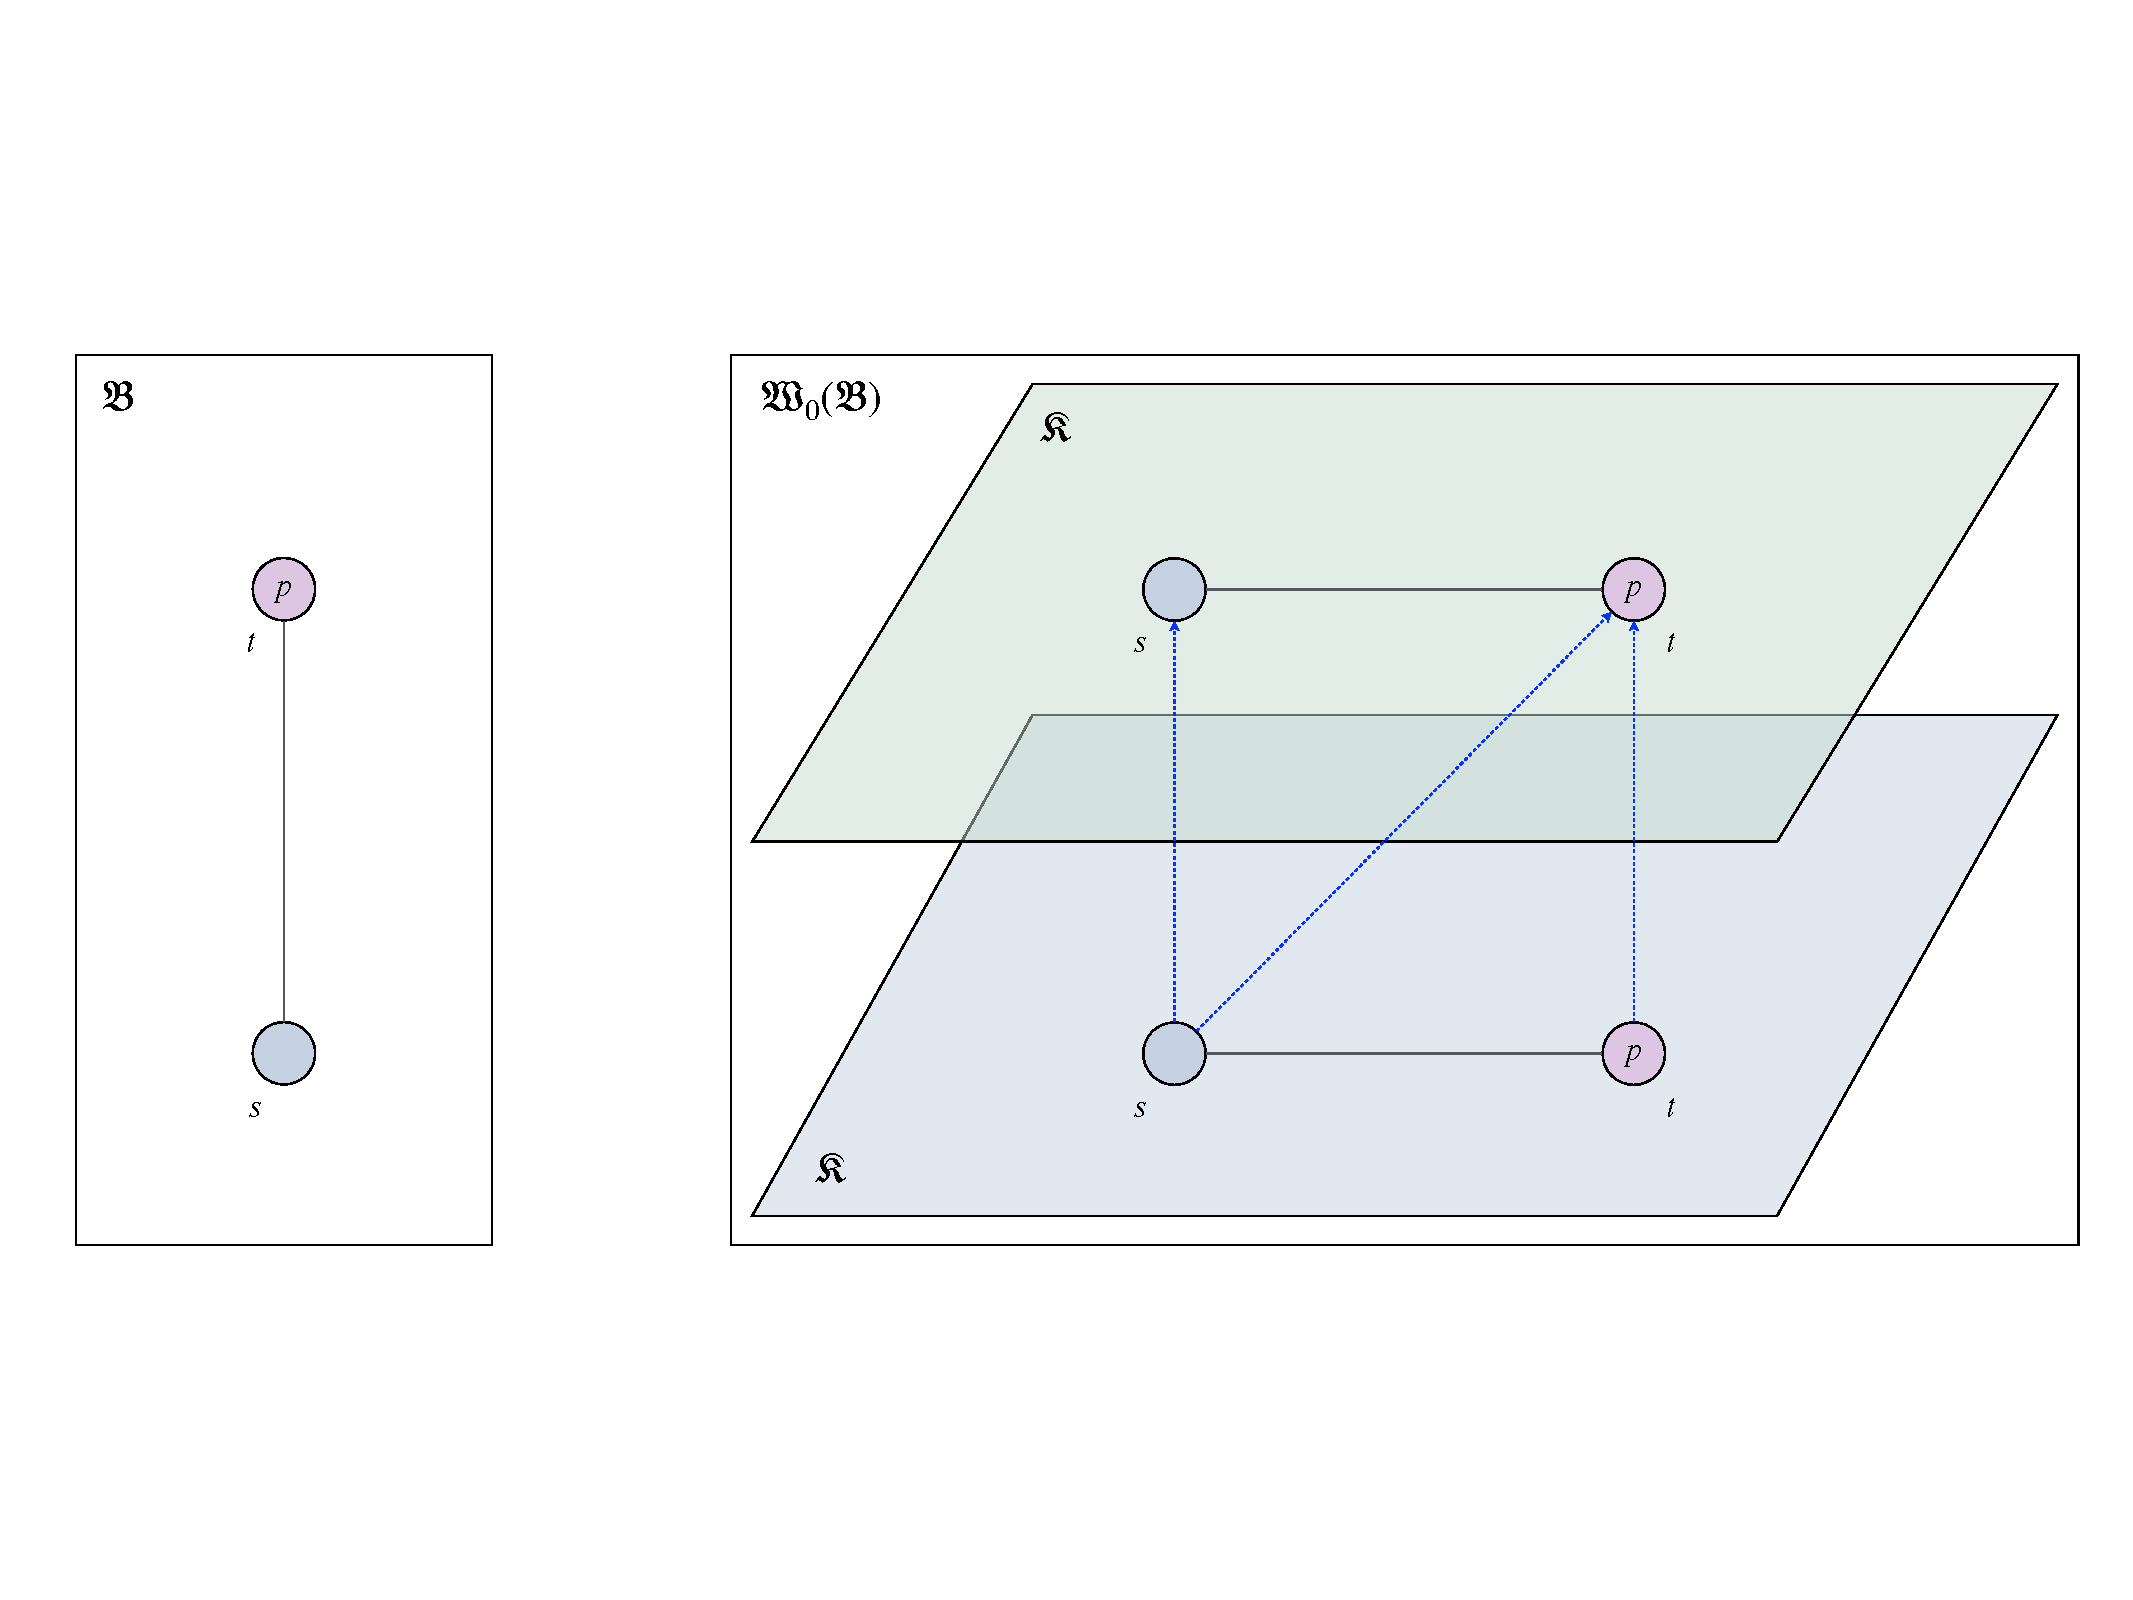
\includegraphics[height=4.9cm]{figures/bks2ws.pdf}
	\caption{Bi-relational Kripke model to Weaved model}
	\label{fig:bks2ws}
\end{figure*}

\begin{example}
        Let $\bmodel$ be the bi-relational model defined by $\Wbm = \set{s, t}$, with $\Fbm = \Delta_{\Wbm} \cup \set{\pair s t}$ and $\Rbm = \set{{\pair s t},{\pair t s}}$. The valuation function is given by $\Vbm(s) = \emptyset$ and $\Vbm(t) = {p}$. This model is depicted on the left side of \Cref{fig:bks2ws}. In the diagram, solid arrows represent the accessibility relation $\Rbm$, and the vertical placement of $t$ above $s$ visually encodes the future pair $s \Fbm t$.

        The weaved model $\wmofbm0$ obtained by applying the construction from \Cref{def:bks2ws} to $\bmodel$ using the trivial partition $\QQs = \set{\set{s, t}}$ is depicted on the right side of \Cref{fig:bks2ws}. In this depiction, the future relation $\Fbm$---now acting as a seesaw simulation from $\kmodel(\set{s, t})$ to itself---is represented by dotted blue arrows.
        To better highlight the hierarchical organization induced by $\Fbm$ within the single Kripke model $\kmodel(\set{s, t}) \in \Kof{\wmofbm0}$, we present it as if there were two stacked copies of the model, rather than illustrating the seesaw simulation as a loop. This visual choice emphasizes the layered nature typical of weaved models.

        \Cref{prop:bks2ws} allows us to compare the evaluation of formulas in $\bmodel$ and $\wmofbm0$.
        It is possible to verify that $\bforces s {\Box\lnot\lnot p}$ and $\nbforces s {\lnot\lnot\Box p}$; and so that $\xforces {\wmofbm0} {\pair {\set{s,t}} s} {\Box\lnot\lnot p}$ and $\nxforces {\wmofbm0} {\pair {\set{s,t}} s} {\lnot\lnot\Box p}$.
        We show the side-by-side evaluation of $\Box\lnot\lnot p$ in $\bmodel$ and $\wmofbm0$ in \Cref{fig:eval}.

        \begin{figure*}
                \begin{center}
                \resizebox{\textwidth}{!}{
                \fbox{
                \begin{minipage}[t]{.55\textwidth}
                        \begin{description}

                        \item[$\bforces s {\Box\lnot\lnot p}$]
                        \item[for all $\Fbm$] \hfil
                        \item[$s \Fbm s$] \hfil
                        \begin{description}
                                \item[for all $\Rbm$]
                                \item[$s \Rbm t$]\hfil
                                \begin{description}
                                \item[$\bforces t {\lnot\lnot p}$]
                                \item[for all $\Fbm$]
                                \item[$t \Fbm t$]\hfil
                                \begin{description}
                                        \item[$\nbforces t {\lnot p}$] \hfil
                                        \begin{description}
                                        \item[exists $\Fbm$]
                                        \item[$t \Fbm t$] \hfil
                                        \item[\quad] $\bforces t p$
                                        \end{description}
                                \end{description}
                                \end{description}
                        \end{description}

                        \item[$s \Fbm t$]\hfil
                        \begin{description}
                                \item[for all $\Rbm$]
                                \item[$t \Rbm s$]\hfil
                                \begin{description}
                                \item[$\bforces s {\lnot\lnot p}$]
                                \item[for all $\Fbm$]
                                
                                \item[$s \Fbm s$]\hfil
                                \begin{description}
                                        \item[$\nbforces s {\lnot p}$] \hfil
                                        \begin{description}
                                        \item[exists $\Fbm$]
                                        \item[$s \Fbm t$] \hfil
                                        \item[\quad] $\bforces t p$
                                        \end{description}
                                \end{description}
                                
                                \item[$s \Fbm t$]\hfil
                                \begin{description}
                                        \item[$\nbforces t {\lnot p}$] \hfil
                                        \begin{description}
                                        \item[exists $\Fbm$]
                                        \item[$t \Fbm t$] \hfil
                                        \item[\quad] $\bforces t p$
                                        \end{description}
                                \end{description}
                                \end{description}
                        \end{description}

                        \end{description}
                \end{minipage}}
                %
                \hfill
                %
                \fbox{
                \begin{minipage}[t]{.55\textwidth}
                        \begin{description}

                        \item[$\xforces {\wmofbm0} {\pair \kmodel s} {\Box\lnot\lnot p}$]
                        \item[for all $\Fof{\wmofbm0}$] \hfil
                        
                        \item[${\pair \kmodel s} \Fof{\wmofbm0} {\pair \kmodel s}$] \hfil
                        \begin{description}
                                \item[for all $\Rkm$]
                                \item[$s \Rkm t$] \hfil
                                \begin{description}
                                \item[$\xforces {\wmofbm0} {\pair \kmodel t} {\lnot\lnot p}$]
                                \item[for all $\Fof{\wmofbm0}$]
                                \item[${\pair \kmodel t} \Fof{\wmofbm0} {\pair \kmodel t}$]\hfil
                                \begin{description}
                                        \item[$\nxforces {\wmofbm0} {\pair \kmodel t} {\lnot p}$]
                                        \item[exists $\Fof{\wmofbm0}$]
                                        \item[${\pair \kmodel t} \Fof{\wmofbm0} {\pair \kmodel t}$]\hfil
                                        \item[\quad] $\xforces {\wmofbm0} {\pair \kmodel t} p$
                                \end{description}
                                \end{description}
                        \end{description}
                        
                        \item[${\pair \kmodel s} \Fof{\wmofbm0} {\pair \kmodel t}$] \hfil
                        \begin{description}
                                \item[for all $\Rkm$]
                                \item[$t \Rkm s$]\hfil
                                \begin{description}
                                \item[$\xforces {\wmodel} {\pair \kmodel s} \lnot\lnot p$]
                                \item[for all $\Fof{\wmofbm0}$]
                                
                                \item[${\pair \kmodel s} \Fof{\wmofbm0} {\pair \kmodel s}$]\hfil
                                \begin{description}
                                        \item[$\nxforces {\wmofbm0} {\pair \kmodel s} {\lnot p}$]
                                        \item[exists $\Fof{\wmofbm0}$]
                                        \item[${\pair \kmodel s} \Fof{\wmofbm0} {\pair \kmodel t}$]\hfil
                                        \item[\quad] $\xforces {\wmofbm0} {\pair \kmodel t} p$
                                \end{description}

                                \item[${\pair \kmodel s} \Fof{\wmofbm0} {\pair \kmodel t}$]\hfil
                                \begin{description}
                                        \item[$\nxforces {\wmofbm0} {\pair \kmodel t} {\lnot p}$]
                                        \item[exists $\Fof{\wmofbm0}$]
                                        \item[${\pair \kmodel t} \Fof{\wmofbm0} {\pair \kmodel t}$]\hfil
                                        \item[\quad] $\xforces {\wmofbm0} {\pair \kmodel t} p$
                                \end{description}
                                \end{description}
                        \end{description}
                        \end{description}
                \end{minipage}}
                }
                \end{center}
                \caption{Side-by-side Evaluation}\label{fig:eval}\lutz{this figure doesn't help at all with the understanding of the paper}
        \end{figure*}
\end{example}

\section{Bisimulation for Weaved models}

% \begin{definition}[\IML-bisimulation]
% 	Let $\wmodel_1 = \tuple{\Kwm[1], \Swm[1]}$ and $\wmodel_2 = \tuple{\Kwm[2], \Swm[2]}$ be two weaved models. Assume that for any $\kmodel_1,\kmodel_2 \in \Kwm[i]$ we have $Q_{\kmodel_1}$ disjoint $Q_{\kmodel_2}$. Define $\bigq[i] = \bigcup_{\kmodel \in \Kwm[i]}Q_{\kmodel}$, and then for $s \in \bigq[i]$ let 
% 	$\kmodel_s$ be the unique model in $\Kwm[i]$ that has $s$ in its domain. An \emph{\IML-bisimulation} between $\wmodel_1$ and $\wmodel_2$ is a non-empty relation $Z \subseteq \bigq[1] \times \bigq[2]$ satisfying the following properties.  Whenever $s Z s'$ then
% 	\begin{description}
%         \setlength{\itemsep}{0pt}
%         \item[\textnormal{(harmony)}] $V_{\kmodel_s}(s) = V_{\kmodel_{s'}}(s')$.
% 		\item[\textnormal{(zig)}] If $s R_{\kmodel_s} t$ then there is $t'$ such that $s' R_{\kmodel_{s'}} t'$ and $t Z t'$.
% 		\item[\textnormal{(zag)}] If $s' R_{\kmodel_{s'}} t'$ then there is $t$ such that $s R_{\kmodel_s} t$ and $t Z t'$.
% 		\item[\textnormal{(s-zig)}] If for some $\Sim$, $s \Sim t$ then there is $t'$ such that 
% 		from some $\Tim$, $s' \Tim t'$ and $t Z t'$.
% 		\item[\textnormal{(s-zag)}] If for some $\Sim$, $s' \Sim t'$ then there is $t$ such that 
% 		from some $\Tim$, $s \Tim t$ and $t Z t'$.
% 	\end{description}
% 	We write $\wmodel_1, s \bisim \wmodel_2, s'$ if there is a bisimulation $Z$ between 
% 	$\wmodel_1$ and $\wmodel_2$ such that $sZs'$.
% \end{definition}

\begin{definition}\label[definition]{def:wbisim}
	A \defn{bisimulation} between weaved models $\wmodel_1$ and $\wmodel_2$, written $Z \colon \wmodel_1 \bisim \wmodel_2$, is a
		non-empty relation $Z \subseteq \Qwm[1] \times \Qwm[2]$ such that,
			for all ${\pair {\kmodel_1} s} \in \Qwm[1]$ and all ${\pair {\kmodel_2} t} \in \Qwm[2]$
				with ${\pair {\kmodel_1} s} Z {\pair {\kmodel_2} t}$:
	\begin{description}
        \setlength{\itemsep}{0pt}
        \item[\textnormal{(harmony)}] $\Vkm[1](s) = \Vkm[2](t)$.
		\item[\textnormal{($\R$-zig)}]
			If there is $u \in \Wkm[1]$ with $s \Rkm[1] u$, then,
				there is $v \in \Wkm[2]$ such that $t \Rkm[2] u$ and ${\pair {\kmodel_1} u} Z {\pair {\kmodel_2} v}$.
		\item[\textnormal{($\R$-zag)}]
			If there is $v \in \Wkm[2]$ with $t \Rkm[2] v$, then,
				there is $u \in \Wkm[1]$ such that $s \Rkm[1] u$ and ${\pair {\kmodel_1} u} Z {\pair {\kmodel_2} v}$.
		\item[\textnormal{($\Fsymb$-zig)}]
			If there are ${\pair {\kmodel_3} u} \in \Qwm[1]$ and ${\Sim\colon \kmodel_1 \fsim \kmodel_3} \in \Swm[1]$ with $s \Sim u$, then,
				there are ${\pair {\kmodel_4} v} \in \Qwm[2]$ and ${\Tim\colon \kmodel_2 \fsim \kmodel_4} \in \Swm[2]$ with $t \Tim v$ and ${\pair {\kmodel_3} u} Z {\pair {\kmodel_4} v}$.
		\item[\textnormal{($\Fsymb$-zag)}]
			If there are ${\pair {\kmodel_4} v} \in \Qwm[2]$ and ${\Tim\colon \kmodel_2 \fsim \kmodel_4} \in \Swm[2]$ with $t \Tim v$, then,
				there are ${\pair {\kmodel_2} u} \in \Qwm[1]$ and ${\Sim\colon \kmodel_1 \fsim \kmodel_3} \in \Swm[1]$ with $s \Sim u$ and ${\pair {\kmodel_3} u} Z {\pair {\kmodel_4} v}$.
	\end{description}
	% We write $Z \colon {\pair {\wmodel_1} {\pair {\kmodel_1} s}} \bisim {\pair {\wmodel_2} {\pair {\kmodel_2} t}}$ if $Z$ is a bisimulation between $\wmodel_1$ and $\wmodel_2$ and ${\pair {\kmodel_1} s} Z {\pair {\kmodel_2} t}$.
\end{definition}

\begin{theorem}[Invariance]
	If $Z \colon \wmodel_1 \bisim \wmodel_2$ and ${\pair {\kmodel_1} s} Z {\pair {\kmodel_2} t}$, then, for all formulas $A$, we have $\xforces {\wmodel_1} {\pair {\kmodel_1} s} A$ iff $\xforces {\wmodel_2} {\pair {\kmodel_1} s} A$.
\end{theorem}
\begin{proof}
    \setcounter{ieqnnum}{0}
    The proof is by induction on $A$.

    \medskip
    \noindent
    The base case is: $\xforces {\wmodel_1} {\pair {\kmodel_1} s} p$ iff $\xforces {\wmodel_2} {\pair {\kmodel_2} t} p$.
	This follows immediately from the (harmony) condition, which guarantees that $\Vkm[1](s) = \Vkm[2](t)$, meaning $s$ and $t$ assign the same truth values to all proposition symbols.

    \medskip
    \noindent
    The inductive step proceeds with a case analysis.
    We prove some representative cases of the kind of reasoning involved.

	\medskip
    \noindent
    For diamonds, we prove $\xforces {\wmodel_1} {\pair {\kmodel_1} s} {\Diamond B}$ implies $\xforces {\wmodel_2} {\pair {\kmodel_2} t} {\Diamond B}$.
    Suppose $\xforces {\wmodel_1} {\pair {\kmodel_1} s} {\Diamond B}$.
    There is $u \in \Wkm[1]$ with \ieqn{s \Rkm[1] u} such that \ieqn{\xforces {\wmodel_1} {\pair {\kmodel_1} u} B}.
	Given \ieqnref{-1}, using the ($\R$-zig) condition, we know that there is \ieqn{v \in \Wkm[2]} with \ieqn{t \Rkm[2] v} such that ${\pair {\kmodel_1} u} Z {\pair {\kmodel_2} v}$.
	By the induction hypothesis, \ieqn{\xforces {\wmodel_2} {\pair {\kmodel_2} v} B}.
	Taken together, \ieqnref{-2}--\ieqnref0 imply $\xforces {\wmodel_2} {\pair {\kmodel_2} t} {\Diamond B}$ as required.
	The converse direction, $\xforces{\wmodel_2}{\pair{\kmodel_2}{t}}{\Diamond B}$ implies $\xforces{\wmodel_1}{\pair{\kmodel_1}{s}}{\Diamond B}$, is established by an analogous argument, this time applying the ($\R$-zag) condition in place of ($\R$-zig).

    \medskip
    \noindent
    For boxes, instead of proving $\xforces {\wmodel_1} {\pair {\kmodel_1} s} {\Box B}$ implies $\xforces {\wmodel_2} {\pair {\kmodel_2} t} {\Box B}$, we prove the contrapositive $\nxforces {\wmodel_2} {\pair {\kmodel_2} t} {\Box B}$ implies $\nxforces {\wmodel_1} {\pair {\kmodel_1} s} {\Box B}$.
    Suppose $\nxforces {\wmodel_2} {\pair {\kmodel_2} t} {\Box B}$.
    There are
		${\pair {\kmodel_4} u} \in \Qwm[2]$
			with \ieqn{{\pair {\kmodel_2} t} \Fwm[2] {\pair {\kmodel_4} u}}, and
		$v \in \Wkm[4]$
			with \ieqn{u \Rkm[4] v} 
	such that
		\ieqn{\nxforces {\wmodel_2} {\pair {\kmodel_4} v} B}.
	From \ieqnref{-2}, we know there is $\Tim\colon\kmodel_2 \fsim \kmodel_4 \in \wmodel_2$ such that $t \Tim u$.
	Given ${\pair {\kmodel_1} s} Z {\pair {\kmodel_2} t}$, the ($\Fsymb$-zag) condition ensures there are ${\pair {\kmodel_3} w} \in \Qwm[1]$ and $\Sim\colon\kmodel_1 \fsim \kmodel_3 \in \wmodel_1$ such that \ieqn{s \Sim w} and \ieqn{{\pair {\kmodel_3} w} Z {\pair {\kmodel_4} u}}.
	Having established \ieqnref{-3} and \ieqnref0, the ($\R$-zag) condition ensures there is $x \in \Wkm[3]$ with \ieqn{w \Rkm[3] x} such that \ieqn{{\pair {\kmodel_3} x} Z {\pair {\kmodel_4} v}}.
	By the inductive hypothesis, \ieqn{\nxforces {\wmodel_1} {\pair {\kmodel_3} x} {B}}.
	Taken together, \ieqnref{-4}, \ieqnref{-2}, and \ieqnref0, imply $\nxforces {\wmodel_1} {\pair {\kmodel_1} s} {\Box B}$ as required.
    The converse direction, $\xforces{\wmodel_2}{\pair{\kmodel_2}{t}}{\Box B}$ implies $\xforces{\wmodel_1}{\pair{\kmodel_1}{s}}{\Box B}$, is established by an analogous argument, this time applying the ($\Fsymb$-zig) and ($\R$-zig) conditions in place of ($\Fsymb$-zag) and ($\R$-zag), respectively.
\end{proof}

%%%% GENERATED WEAVED model

\begin{definition}\label[definition]{def:gen:wmodel}
    Let $\wmodel$ be a weaved model.
	For any $\kmodel \in \Kwm$, define the \defn{restriction} of $\wmodel$ to $\kmodel$ as a pair $\rwmodel = \tuple{\Krwm, \Srwm}$ where:
    \begin{enumerate}[leftmargin=\parindent]
        \setlength{\itemsep}{0pt}
        \item $\Krwm = \setof{\kmodel'}{\mbox{there is } {\Sim \colon \kmodel \fsim \kmodel'} \in \Swm}$; and
        \item $\Srwm = \Swm \cap (\Krwm \times \Krwm)$
    \end{enumerate}
    We also call $\rwmodel$ the \defn{$\kmodel$-generated weaved submodel} of $\wmodel$, or simply a generated weaved submodel if $\wmodel$ and $\kmodel$ are understood from the context.
\end{definition}

\begin{proposition}\label[proposition]{prop:bisim:rwmodel}
	Let $\wmodel$ be a weaved model.
	For all $\kmodel \in \Kwm$, the relation $Z = \setof{\pair {\pair {\kmodel'} s} {\pair {\kmodel'} s}}{ {\pair {\kmodel'} s} \in \Qof{\rwmodel}}$ is a bisimulation between $\rwmodel$ and $\wmodel$.
\end{proposition}

\begin{corollary}\label[corollary]{prop:rwmodel}
    For all formulas $A$, we have $\wforces{\pair \kmodel s}{A} \mbox{ iff } \xforces{\rwmodel}{\pair \kmodel s}{A}$.
\end{corollary}

%%%% UNRAVELING WEAVED model

\begin{definition}\label[definition]{def:unraveling}
	Let $\wmodel$ be a weaved model and let $\kmodel \in \Kwm$.
	To properly define the unraveling of $\wmodel$ around $\kmodel$, we first need to introduce a few preliminary notions.
        \lutz{that's not a definition} \lutz{and never write a definition that spans more than a page}

	\medskip
	\noindent
	By a \defn{simulation thread} starting at $\kmodel$ we mean a finite sequence $\pi = \Sim_1 \dots \Sim_n$ of simulations in $\Swm$ such that: $\dom(\Sim_1) = \kmodel$, and the composition ${\Sim_1 \dots \Sim_n \in \Swm}$.
	We take the empty sequence, denoted by $\varepsilon$, to stand for the starting model $\kmodel$.
	We use $|\pi|$ to indicate the length of a thread $\pi$.
	For each $i \in [1{:}|\pi|]$, we let $\pi_i$ be the codomain of the $i$-th simulation in $\pi$, that is, $\pi_i = \cod(\Sim_i) = \kmodel_i$, with the convention $\pi_0 = \kmodel$.
	We write $\pi[{:}i]$ to denote the initial segment of $\pi$ up to the $i$-th simulation, that is, $\pi[{:}i] = \Sim_1 \dots \Sim_i$, with the convention $\pi[{:}0] = \varepsilon = \kmodel$.
	Finally, we use $\Pi$ to denote the collection of all such simulation threads in $\wmodel$.
	Intuitively, simulation threads make paths in the weaved model explicit: they record step by step how one moves through the model. As we will show below, simulation threads provide the fundamental building blocks for the unraveling construction.
	
	\medskip
	\noindent
	To transform abstract simulation threads into concrete components of the unraveling, we tie each thread to a unique copy of the Kripke model it reaches. To achieve this, we associate to a each $\pi \in \Pi$ a set $\Qof{\pi} = \setof{s_{\pi}}{s \in \Qof{\pi_{|\pi|}}}$ and a bijection $f_{\pi}\colon {\Qof{\pi_{|\pi|}} \bsym \Qof{\pi}}$ such that $f_{\pi}(s) = s_\pi$.
	This definition of $f_{\pi}$ provides us with a systematic way of generating the unique Kripke models that will play the role of the nodes of tree-like model characteristic of unravelings.

	\medskip
	\noindent
	Concretely, every $f_{\pi}$ yields a Kripke model $\kmodel_{\pi} = \tuple{\Qof{\pi}, \Rof{\pi}, \Vof{\pi}}$ where:
	\begin{enumerate}[leftmargin=\parindent,resume]
        \setlength{\itemsep}{0pt}
		% \item $\Qof{\pi} = \cod(f_{\pi})$;
		\item $\Rof{\pi} = \setof{\pair {s_\pi} {t_\pi}}{ s \Rof{\pi_{|\pi|}} t}$; and
		\item for all $s_{\pi} \in \Qof{\pi}$, $\Vof{\pi}(s_{\pi}) = \Vof{\pi_{|\pi|}}(s)$.
	\end{enumerate}
	It is immediate from the definition of $f_{\pi}$ that each $\kmodel_{\pi}$ is indeed a unique isomorphic copy of $\pi_{|\pi|}$.

	\medskip
	\noindent
	Having identified the Kripke models that will appear in the unraveling, we turn to defining the simulations that will connect these models together. Intuitively, these simulations must branch in a disciplined manner so that, taken as a whole, they generate the tree-like shape characteristic of unravelings.
	The key lies in the notion of an extension of a simulation thread.
	
	\medskip
	\noindent
	We say that a simulation thread $\pi'$ is an \defn{extension} of a simulation thread $\pi$ iff $\pi = \pi'[{:}|\pi|]$. We write $\pi\pi'$ if $\pi'$ is an extension of $\pi$. Extensions provide the natural mechanism for controlling how simulations branch in the unraveling.

	\medskip
	\noindent
	Concretely, for every pair $\pi\pi'$ with $\pi' = \Sim_1 \dots \Sim_{|\pi|} \Sim_{(|\pi|+1)} \dots \Sim_{|\pi'|}$, we define
	\begin{enumerate}[leftmargin=\parindent,resume]
        \setlength{\itemsep}{0pt}
		\item $\Sim_{\pi\pi'} = f_{\pi}^{-1} \Sim_{(|\pi|+1)} \dots \Sim_{|\pi'|} f_{\pi'}$.
	\end{enumerate}
	It follows directly from the definition that $\Sim_{\pi\pi'}$ is a simulation from $\kmodel_{\pi}$ to $\kmodel_{\pi'}$.
	Composition of these simulations is defined in the natural way: for any $\pi, \pi', \pi'' \in \Pi$, we set $\Sim_{\pi\pi'}\Sim_{\pi'\pi''} = \Sim_{\pi\pi''}$. This composition is clearly well-defined.
	In addition, for every $\pi \in \Pi$, there exists a simulation $\Sim_{\pi\pi}$ that behaves as an identity: for all $\pi' \in \Pi$, if $\pi'$ is an extension of $\pi$, then, $\Sim_{\pi\pi}\Sim_{\pi\pi'} = \Sim_{\pi\pi'}$; and if $\pi$ is an extension of $\pi'$, then, $\Sim_{\pi'\pi}\Sim_{\pi\pi} = \Sim_{\pi'\pi}$.
	Thus, $\Sim_{\pi\pi}$ serves as the identity simulation for $\kmodel_{\pi}$.

	\medskip
	\noindent
	Having set up the necessary definitions, we can now put them together into the unraveling of $\wmodel$ around $\kmodel$. This construction turns the abstract machinery developed above into a tree-like model that makes explicit how simulation threads unfold.
	Precisely, we define the \defn{unraveling} of $\wmodel$ around $\kmodel$ as a pair $\uwmodel = \tuple{\Kuwm, \Suwm}$ where:
	\begin{enumerate}[leftmargin=\parindent,resume]
        \setlength{\itemsep}{0pt}
		\item $\Kuwm = \setof{\kmodel_\pi}{\pi \in \Pi}$;
		\item $\Suwm = \setof{\Sim_{\pi\pi'}}{\pi,\pi' \in \Pi \mbox{ and } \pi' \mbox{ is an extension of } \pi}$.
	\end{enumerate}
\end{definition}

\begin{proposition}
	The unraveling of a weaved model $\wmodel$ around a Kripke model $\kmodel \in \Kwm$ is a weaved model.
\end{proposition}
% \begin{proof}
% 	\setcounter{ieqnnum}{0}
% 	By construction, each $\kmodel_\pi \in \Kuwm$ is a Kripke model.
% 	The non-trivial part is to prove that each $\Sim^i_\pi \in \Suwm$ is a seesaw simulation from $\kmodel_{\pi[i]}$ to $\kmodel_\pi$. %, i.e., $\Sim^i_\pi \colon \kmodel_{\pi[i]} \fsim \kmodel_\pi$.
% 	To establish this, we must verify:
% 	\ieqn{\Sim^i_\pi \subseteq \Qof{\pi[i]} \times \Qof{\pi}}; and
% 	\ieqn{\Sim^i_\pi} satisfies conditions (add), (see), and (saw) of seesaw simulations.
% 	Condition \ieqnref{-1} follows directly from the definition of $\Sim^i_\pi$.
% 	We establish $\Sim^i_\pi$ is a simulation below.

% 	\medskip
% 	\noindent
% 	To simplify notation, let
% 		\ieqn{\pi = \kmodel_1 \Sim_1 \dots \Sim_{(n-1)} \kmodel_n}.
% 	Moreover, let
% 		\ieqn{\Sim = (\Sim_i \fcomp \dots \Sim_n)\colon \kmodel_i \fsim \kmodel_n \in \Swm}.

% 	\medskip
% 	\noindent
% 	For (add), choose an arbitrary $s \Sim^i_\pi t$.
% 	We must prove $\Vof{\pi[i]}(s) \subseteq \Vof{\pi}(t)$.
% 	By definition $\Vof{\pi[i]}(s) = \Vkm[i](s)$, and $\Vof{\pi}(t) = \Vkm[n](t)$.
% 	The result follows directly from the (add) condition in \ieqnref0.
	
% 	\medskip
% 	\noindent
% 	For (see), again choose an arbitrary $s \Sim^i_\pi t$.
% 	By definition, from \ieqnref0, we have $s_i \Sim t_n$.
% 	Take $u \in \Qof{\pi[i]}$ such that $s \Rof{\pi[i]} u$.
% 	This scenario is best illustrated by the following arrow-chasing diagram, which displays how the prefix $\pi[i]$ aligns with the full thread $\pi$ via the simulations~in~$\Sim$:
% 	\[
% 		\begin{tikzcd}
% 			s_1
% 				\arrow[r,dotted, "\Sim_1"]
% 				\arrow[d, swap, "{\Rkm[1]}" {yshift=1pt}]
% 			% &
% 			% s_2
% 			% 	\arrow[r,dotted, "\Sim_2" {xshift=-2pt}]
% 			% 	\arrow[d, "\Rof{\pi_2}" {yshift=1pt}]
% 			&
% 			\dots
% 				\arrow[r,dotted, "\Sim_{(i-1)}" {xshift=-2pt}]
% 			&
% 			s_i
% 				\arrow[r,dotted, "\Sim_i"]
% 				\arrow[rr, bend left=35,dotted, "\Sim"]
% 				\arrow[d, swap, "{\Rkm[i]}" {yshift=1pt}]
% 			% &
% 			% s_{(i+1)}
% 			% 	\arrow[r,dotted, "\Sim_{(i+1)}" {xshift=-2pt}]
% 			% 	\arrow[d, "\Rof{\pi_{(i+1)}}" {yshift=1pt}]
% 			&
% 			\dots
% 				\arrow[r,dotted, "\Sim_{(n-1)}" {xshift=-2pt}]
% 			&
% 			t_{n}
% 				\arrow[d, "{\Rkm[n]}" {yshift=1pt}]
% 			\\
% 			u_1
% 				\arrow[r, swap, dotted, "\Sim_1"]
% 			% &
% 			% u_2
% 			% 	\arrow[r, swap, dotted]{}{\Sim_2}
% 			&
% 			\dots
% 				\arrow[r, swap, dotted, "\Sim_{(i-1)}" {xshift=-2pt}]
% 			&
% 			u_i
% 				\arrow[r, swap, dotted, "\Sim_i"]
% 				\arrow[rr, bend left=35,dotted, "\Sim"]
% 			% &
% 			% u_{(i+1)}
% 			% 	\arrow[r, swap, dotted]{}{\Sim_{(i+1)}}
% 			&
% 			\dots
% 				\arrow[r, swap, dotted, "\Sim_{(n-1)}" {xshift=-2pt}]
% 			&
% 			u_{n}
% 		\end{tikzcd}
% 	\]
% 	Formally, $s \Rof{\pi[i]} u$ ensures that the tuple $s_1,\dots,s_i$ is linked step by step to $u_1,\dots,u_i$ through the chain of simulations.
% 	Then, $s \Sim^i_\pi t$ implies, using the (see) condition for $\Sim$, that the tuple $s_1,\dots,s_i,\dots,s_n$ extends coherently along the entire thread, yielding the sequence $v = u_1 \dots u_n \in \Qof{\pi}$.
% 	Consequently, we obtain both $t \Rof{\pi} v$ and $u \Sim^i_\pi v$, exactly as required for condition (see).
% 	The argument for (saw) is entirely analogous using the (saw) condition in $\Sim$ instead of (see) in $\Sim$.

% 	\medskip
% 	\noindent
% 	To conclude the proof we must prove that $\Suwm$ is closed under identities and composition.
% 	It is clear that $\Sim^1_\pi \in \Suwm$ acts as the identity on $\kmodel_\pi$.
% 	For composition, we note that $\Sim^i_{\pi}\colon \kmodel_{\pi[i]} \fsim \kmodel_{\pi}$ and $\Tim^j_{\pi'}\colon \kmodel_{\pi'[j]} \fsim \kmodel_{\pi'}$ can be composed only if $\pi = \pi'[j]$.
% 	Then, we define $s (\Sim^i_{\pi} \fcomp \Tim^j_{\pi'}) t$ iff the following conditions are met:
% 	\begin{enumerate}[leftmargin=\parindent,label=(\alph*)]
%         \setlength{\itemsep}{0pt}
% 		\item $s \in \Qof{\pi[i]}$;
% 		\item $t \in \Qof{\pi'}$; and
% 		\item exists $u \in \Qof{\pi}$ such that $s_i (\Sim_i \fcomp \dots \fcomp \Sim_{(|\pi|-1)}) u_{|\pi|} (\Tim_j \fcomp \dots \fcomp \Tim_{|\pi'|}) t_{|\pi'|}$.
% 	\end{enumerate}
% \end{proof}

\begin{proposition}\label[proposition]{prop:bisim:uwmodel}
	Let $\rwmodel$ be a $\kmodel$-generated weaved model.
	Then, for all
		$\pair {\kmodel'} s \in \Qof{\rwmodel}$ and all
		$\pair {\kmodel_\pi} t \in \Qof{\uwmodel}$,
	define
		\[
			{{\pair {\kmodel'} s} Z {\pair {\kmodel_{\pi}} {s_{\pi}}}}
			\quad
			\mbox{iff}
			\quad
			{\kmodel' = \pi_{|\pi|}}
		\]
	It follows that $Z$ is a bisimulation between $\rwmodel$ and $\uwmodel$.
\end{proposition}
\begin{proof}
	The key observation is that $Z$ provides a pointwise correspondence between the Kripke models in the generated weaved model and their isomorphic copies in the unraveling. This correspondence immediately guarantees the ($\R$-zig) and ($\R$-zag) conditions of a bisimulation.

	\medskip
	\noindent
	In turn, consider ${\Sim \colon \kmodel' \fsim \kmodel''} \in \Srwm$. Then, extending $\pi$ by $\Sim$ yields a simulation thread $\pi' = \pi\Sim \in \Pi$. This extension ensures the unraveling includes the simulation ${\Sim_{\pi\pi'} \colon \kmodel_\pi \fsim \kmodel_{\pi'}} \in \Suwm$, which guarantees ($\Fsymb$-zig).

	\medskip
	\noindent
	Conversely, given ${\Tim \colon \kmodel_{\pi'} \fsim \kmodel_{\pi''}} \in \Suwm$, we can move back to the weaved model: the bijections $f_{\pi'}$ and $f_{\pi''}$ ensure the existence of the simulation ${\Sim = f_{\pi'} \Tim f_{\pi''}^{-1} \colon \kmodel' \fsim \pi''_{|\pi''|}} \in \Srwm$, which provides ($\Fsymb$-zag).
\end{proof}

\begin{corollary}\label[corollary]{prop:uwmodel}
	For all formulas $A$, $\xforces{\rwmodel}{\pair \kmodel s}{A}$ iff $\xforces{\uwmodel}{\pair {\kmodel_{\varepsilon}} {s_{\varepsilon}}}{A}$.
\end{corollary}

\begin{definition}\label[definition]{def:idepth}
	The \defn{intuitionistic degree} of a formula $A$ is defined as:
	\begin{align*}
		\ideg(p) & = 0 \\
		\ideg(\bot) & = 0 \\
		\ideg(B \lor C) &= \max(\ideg(B),\ideg(C)) \\
		\ideg(B \land C) &= \max(\ideg(B),\ideg(C)) \\
		\ideg(B \to C) &= 1+\max(\ideg(B),\ideg(C)) \\
		\ideg(\Diamond B) &= \ideg(B) \\
		\ideg(\Box B) &= 1+ \ideg(B)
	\end{align*}
\end{definition}

\begin{definition}\label[definition]{def:nbisimulation}
	Let $\wmodel_1$ and $\wmodel_2$ be weaved models.
	Suppose we are given a finite sequence of non-empty relations $Z^n \subseteq Z^{(n-1)} \subseteq \dots \subseteq Z^0$ on $\Qwm[1] \times \Qwm[2]$, where each $Z^i$ satisfies the conditions (harmony), ($\R$-zig), and ($\R$-zag) from \Cref{def:wbisim}.
	We say that $Z^n$ is an \defn{$n$-bisimulation} between $\wmodel_1$ and $\wmodel_2$, and write $Z^n \colon \wmodel_1 \bisim^n \wmodel_2$, iff for all $i \in [1{:}n]$, and all ${\pair {\kmodel_1} s} \in \Qwm[1]$ and ${\pair {\kmodel_2} t} \in \Qwm[2]$ with ${\pair {\kmodel_1} s} Z^i {\pair {\kmodel_2} t}$, the following holds:
	\begin{description}
        \setlength{\itemsep}{0pt}
		\item[\textnormal{($\Fsymb^i$-zig)}]
			If there are ${\pair {\kmodel_3} u} \in \Qwm[1]$ and ${\Sim\colon \kmodel_1 \fsim \kmodel_3} \in \Swm[1]$ with $s \Sim u$, then,
				exist ${\pair {\kmodel_4} v} \in \Qwm[2]$ and ${\Tim\colon \kmodel_2 \fsim \kmodel_4} \in \Swm[2]$ with $t \Tim v$ and ${\pair {\kmodel_3} u} Z^{(i-1)} {\pair {\kmodel_4} v}$.
		\item[\textnormal{($\Fsymb^i$-zag)}]
			If there are ${\pair {\kmodel_4} v} \in \Qwm[2]$ and ${\Tim\colon \kmodel_2 \fsim \kmodel_4} \in \Swm[2]$ with $t \Tim v$, then,
				exist ${\pair {\kmodel_2} u} \in \Qwm[1]$ and ${\Sim\colon \kmodel_1 \fsim \kmodel_3} \in \Swm[1]$ with $s \Sim u$ and ${\pair {\kmodel_3} u} Z^{(i-1)} {\pair {\kmodel_4} v}$.
	\end{description}
\end{definition}

\begin{theorem}[$n$-invariance]\label[theorem]{prop:ninv}
	If $Z^n \colon \wmodel_1 \bisim^n \wmodel_2$ and ${\pair {\kmodel_1} s} Z^n {\pair {\kmodel_2} t}$, then, for all formulas $A$ with $\ideg(A) \leq n$, we have $\xforces {\wmodel_1} {\pair {\kmodel_1} s} A$ iff $\xforces {\wmodel_2} {\pair {\kmodel_1} s} A$.
\end{theorem}
\begin{proof}
    \setcounter{ieqnnum}{0}
    The proof is by induction on two measures: the degree and the size of the formula $A$.
	Precisely, we associate with each formula $A$ a complexity pair $\pair {\deg(A)} {\size(A)}$, the proof is by strong induction on the lexicographic order on such pairs.

    \medskip
    \noindent
    For the base case we need to establish $\xforces {\wmodel_1} {\pair {\kmodel_1} s} p$ iff $\xforces {\wmodel_2} {\pair {\kmodel_2} t} p$.
	This follows directly from the (harmony) condition in $Z^0$, which guarantees that $\Vkm[1](s) = \Vkm[2](t)$, meaning $s$ and $t$ assign the same truth values to all proposition symbols.

    \medskip
    \noindent
    For the inductive step, we choose a pair ${\pair {\kmodel_1} s} Z^{(i+1)} {\pair {\kmodel_2} t}$, and a formula $A$ with complexity $(i+1,j)$. The inductive hypothesis tells us that the result holds for all pairs ${\pair {\kmodel_3} u} Z^i {\pair {\kmodel_4} v}$ and all formulas with complexity $(k,\ell) < (i+1,j)$. We are required to prove that the result holds for $A$. We proceed with a case analysis.

	\medskip
    \noindent
    For conjunctions, we prove $\xforces{\wmodel_1}{\pair{\kmodel_1}{s}}{B \land C}$ implies $\xforces{\wmodel_2}{\pair{\kmodel_2}{t}}{B \land C}$.
	Suppose $\xforces{\wmodel_1}{\pair{\kmodel_1}{s}}{B \land C}$.
	By the semantics of conjunction, this means that $\xforces{\wmodel_1}{\pair{\kmodel_1}{s}}{B}$ and $\xforces{\wmodel_1}{\pair{\kmodel_1}{s}}{C}$.
	The complexity pairs associated with $B$ and $C$ both precede $(i+1,j)$ in the lexicographic order.
	Therefore, by the inductive hypothesis, we obtain $\xforces{\wmodel_2}{\pair{\kmodel_2}{t}}{B}$ and $\xforces{\wmodel_2}{\pair{\kmodel_2}{t}}{C}$. Together, these yield $\xforces{\wmodel_2}{\pair{\kmodel_2}{t}}{B \land C}$.
	The converse direction, $\xforces{\wmodel_2}{\pair{\kmodel_2}{t}}{B \land C}$ implies $\xforces{\wmodel_1}{\pair{\kmodel_1}{s}}{B \land C}$, follows by an entirely symmetric argument.
	The case for disjunctions proceeds in exactly the same way.

	\medskip
    \noindent
    For diamonds, we prove $\xforces {\wmodel_1} {\pair {\kmodel_1} s} {\Diamond B}$ implies $\xforces {\wmodel_2} {\pair {\kmodel_2} t} {\Diamond B}$.
    Suppose $\xforces {\wmodel_1} {\pair {\kmodel_1} s} {\Diamond B}$.
    There is $u \in \Wkm[1]$ with \ieqn{s \Rkm[1] u} such that \ieqn{\xforces {\wmodel_1} {\pair {\kmodel_1} u} B}.
	Given \ieqnref{-1}, using the ($\R$-zig) condition in $Z^{(i+1)}$, we know that there is \ieqn{v \in \Wkm[2]} with \ieqn{t \Rkm[2] v} such that ${\pair {\kmodel_1} u} Z^{(i+1)} {\pair {\kmodel_2} v}$.
	Now, the complexity pair associated with $B$ precedes $(i+1,j)$ in the lexicographic order.
	Therefore, by the induction hypothesis, \ieqn{\xforces {\wmodel_2} {\pair {\kmodel_2} v} B}.
	Taken together, \ieqnref{-2}--\ieqnref0 imply $\xforces {\wmodel_2} {\pair {\kmodel_2} t} {\Diamond B}$ as required.
	The converse direction, $\xforces{\wmodel_2}{\pair{\kmodel_2}{t}}{\Diamond B}$ implies $\xforces{\wmodel_1}{\pair{\kmodel_1}{s}}{\Diamond B}$, is established by an analogous argument, this time using ($\R$-zag) in place of ($\R$-zig).

    \medskip
    \noindent
    For boxes, instead of proving $\xforces {\wmodel_1} {\pair {\kmodel_1} s} {\Box B}$ implies $\xforces {\wmodel_2} {\pair {\kmodel_2} t} {\Box B}$, we prove the contrapositive $\nxforces {\wmodel_2} {\pair {\kmodel_2} t} {\Box B}$ implies $\nxforces {\wmodel_1} {\pair {\kmodel_1} s} {\Box B}$.
    Suppose $\nxforces {\wmodel_2} {\pair {\kmodel_2} t} {\Box B}$.
    There are
		${\pair {\kmodel_4} u} \in \Qwm[2]$ with
			\ieqn{{\pair {\kmodel_2} t} \Fwm[2] {\pair {\kmodel_4} u}}, and
		$v \in \Wkm[4]$ with
			\ieqn{u \Rkm[4] v} 
		such that
			\ieqn{\nxforces {\wmodel_2} {\pair {\kmodel_4} v} B}.
	From \ieqnref{-2}, exists $\Tim\colon\kmodel_2 \fsim \kmodel_4 \in \wmodel_2$ such that $t \Tim u$.
	Since ${\pair {\kmodel_1} s} Z^{(i+1)} {\pair {\kmodel_2} t}$, the ($\Fsymb^{(i+1)}$-zag) condition ensures there are
		${\pair {\kmodel_3} w} \in \Qwm[1]$ and
		$\Sim\colon\kmodel_1 \fsim \kmodel_3 \in \wmodel_1$
		such that
			\ieqn{s \Sim w} and
			\ieqn{{\pair {\kmodel_3} w} Z^i {\pair {\kmodel_4} u}}.
	Now, \ieqnref{-3} and \ieqnref0 imply, by the ($\R$-zag) condition in $Z^i$,
		there are
			$x \in \Wkm[3]$
			such that
				\ieqn{w \Rkm[3] x} and
				\ieqn{{\pair {\kmodel_3} x} Z^i {\pair {\kmodel_4} v}}.
	Since $\ideg(B) = i$, by the induction hypothesis, we obtain
		\ieqn{\nxforces{\wmodel_1}{\pair {\kmodel_3} {x}}{B}}.
	Taken together, \ieqnref{-4}, \ieqnref{-2}, and \ieqnref0, imply $\nxforces {\wmodel_1} {\pair {\kmodel_1} s} {\Box B}$ as required.
    The converse direction, $\xforces{\wmodel_2}{\pair{\kmodel_2}{t}}{\Box B}$ implies $\xforces{\wmodel_1}{\pair{\kmodel_1}{s}}{\Box B}$, is established by an analogous argument, this time applying the ($\Fsymb$-zig) and ($\R$-zig) conditions in place of ($\Fsymb$-zag) and ($\R$-zag), respectively.
\end{proof}

\begin{definition}\label[definition]{def:prunning}
	Let $\uwmodel$ be the unraveling of a weaved model $\wmodel$ around a Kripke model $\kmodel \in \Kwm$.
	The \defn{prunning} of $\uwmodel$ at height $n$ is a weaved model $\pwmodel = \tuple{\Kpwm, \Spwm}$ where:
	\begin{enumerate}[leftmargin=\parindent]
		\setlength{\itemsep}{0pt}
		\item For all $\kmodel_{\pi} \in \Kuwm$, $|\pi| \leq n$ implies $\kmodel_{\pi} \in \Kpwm$;
		\item For all $\Sim\colon\kmodel_{\pi}\fsim\kmodel_{\pi'} \in \Suwm$, if $\kmodel_{\pi},\kmodel_{\pi'} \in \Kpwm$, then, $\Sim \in \Sbwm$.
	\end{enumerate}
\end{definition}

\begin{proposition}\label[proposition]{prop:bounded:height}
	Let $\uwmodel$ be the unraveling of a weaved model $\wmodel$ around a Kripke model $\kmodel \in \Kwm$.
	For all $i \in [0{:}n]$, define 
	\[ Z^i = \setof{\pair {\pair {\kmodel_{\pi}} s} {\pair {\kmodel_{\pi}} s}}{ \kmodel_{\pi} \in \Kuwm \mbox{ and } |\pi| \leq (n-i)} \]
	It follows that:
	\begin{enumerate}[leftmargin=\parindent]
		\setlength{\itemsep}{0pt}
		\item $Z^{n} \subseteq Z^{(n-1)} \subseteq \dots \subseteq Z^0$ is a finite sequence of non-empty relations on $\Qof{\uwmodel} \times \Qof{\pwmodel}$ each of which satisfies the conditions (harmony), ($\R$-zig), and ($\R$-zag) in \Cref{def:wbisim};
		\item $Z^n \colon \uwmodel \bisim^n \pwmodel$; and
		\item ${\pair {\kmodel_{\pi}} s} Z^k {\pair {\kmodel_{\pi}} s}$ where $k = n - |\pi|$.
	\end{enumerate}
\end{proposition}

\lutz{it's not really clear what the motivation for this unravelling is}

\begin{corollary}\label[corollary]{prop:pwmodel}
	For all formulas $A$, if $\ideg(A) \leq n$, then, $\xforces{\uwmodel}{\pair {\kmodel_{\varepsilon}} {s_{\varepsilon}}}{A}$ iff $\xforces{\pwmodel}{\pair {\kmodel_{\varepsilon}} {s_{\varepsilon}}}{A}$.
\end{corollary}

\section{Filtrations on Weaved models}\label[section]{sec:filtrations}

In this section, we establish the \emph{finite model property} for \IML by exploiting the layered architecture of weaved models. This result is of immediate significance since it yields \emph{decidability}. Equally important, however, is the proof method we adopt. Our argument is based on \emph{filtrations}, a classical technique from modal logic that constructs finite models by identifying worlds that agree on the truth of a fixed, subformula-closed set of formulas. Adapting filtrations to intuitionistic modal semantics has long been known to be challenging. In particular, as discussed in \cite{simpson1994}, an early attempt by Ewald to extend the classical filtration method to bi-relational models was later shown to be flawed. Here, We show that weaved models provide a natural and robust setting in which intuitionistic filtrations can be carried out successfully. Their layered, simulation-based architecture supports a direct and technically well-behaved filtration construction, avoiding earlier difficulties and yielding a streamlined proof of the finite model property---and hence decidability---for \IML.

We begin by precisely defining what we mean by a finite weaved model.

\begin{definition}
    We say that a Kripke model $\kmodel$ is \defn{finite} iff $\Wkm$ is finite.
    We say that a weaved model is \defn{finite} iff all Kripke models in $\Kwm$ are finite.
\end{definition}

Finiteness in weaved models reflects their layered architecture. In brief, two requirements must be satisfied: each individual Kripke model must contain only finitely many worlds, and the collection of Kripke models making up the weaved model must itself be finite. These conditions capture two complementary aspects of finiteness: horizontally, each slice is a finite collection of finite Kripke model; vertically, the number of slices, i.e., the layers of the weave model, is bounded in size. Paying attention to both directions of finiteness is crucial for establishing the finite model property in this framework.
Having clarified the two-dimensional notion of finiteness, we introduce the filtration construction for weaved models, and prove how it provides a mechanism for controlling both dimensions simultaneously.

\begin{proposition}
    Let $\wmodel$ be a weaved model, and $\fset$ be a set of formulas closed under subformulas.
    For any Kripke model $\kmodel \in \Kwm$, we define a binary relation $\feqr$ on $\Wkm$ such that $s \feqr t$ iff for all $A \in \fset$, $\wforces {\pair \kmodel s} A$ iff $\wforces {\pair \kmodel t} A$.
    It follows that every $\feqr$ is an equivalence relation.
\end{proposition}

\begin{proposition}
    Let $\wmodel$ be a weaved model, and $\fset$ be a set of formulas closed under subformulas.
    For any Kripke model $\kmodel \in \Kwm$, and any $s \in \Wkm$, let $\feqc{s}$ be the equivalence class of $s$ under $\feqr$.
    Then, we define $\fmodel = \tuple{\Wfm, \Rfm, \Vfm}$ where:

        \begin{enumerate}
            \item $\Wfm = \setof{\feqc{s}}{s \in \Wkm}$.
            \item $\Rfm = \setof{\pair {\feqc{s}} {\feqc{t}}}{ \mbox{there are $s' \in \feqc{s}$ and $t' \in \feqc{t}$ such that $s' \Rkm t'$}}$.
            % \carlos{One way of defining this, just to try.    We can later do the usual range of possible definitions for relations.}
            \item $\Vfm \colon \Wfm \to 2^{\props}$ is such that for all $\feqc{s} \in \W$, $\V(\feqc{s}) = \Vkm(s) \cap \Sigma$.
        \end{enumerate}
    
    \noindent
    It follows that $\fmodel$ is a Kripke model.
\end{proposition}
\begin{proof}
    We only need to check that the function $\Vfm$ is well-defined, that is, that the selection of the representative for $\feqc{s}$ has no impact in the definition of $\Vfm(\feqc{s})$.
    But this is immediate from the fact that any such a representative agrees on $\fset$.
\end{proof}

\begin{definition}
    For any weaved model $\wmodel$, and any set of formulas $\Sigma$, closed under subformulas, we define the \defn{filtration} of $\wmodel$ through $\Sigma$ to be the weaved model $\fwmodel = \tuple{\Kfwm, \Sfwm}$, where:
    \begin{enumerate}[leftmargin=\parindent]
        \setlength{\itemsep}{0pt}
        \item $\Kfwm = \setof{\fmodel}{\kmodel \in \Kwm}$;
        
        \item $\Sfwm$ is the smallest set such that for all $\Sim \colon \kmodel_1 \fsim \kmodel_2 \in \Swm$,
            $\fSim \in \Sfwm$.
    \end{enumerate}
    When $\wmodel$ can be understood from the context, we refer to $\fwmodel$ as the $\Sigma$-filtered weaved model.
\end{definition}

The next two results establish that weaved models are well-suited for applying the filtration method.

\begin{proposition}\label[proposition]{prop:filtration}
    $\Sigma$-filtrations are weaved models.
    % The filtration $\fwmodel$ of a weaved model $\wmodel$ with respect to a set of formulas $\Sigma$ closed under subformulas is itself a weaved model.
\end{proposition}
\begin{proof}
    \setcounter{ieqnnum}{0}
    We need to check:
        (a) every $\fmodel \in \Kfwm$ is a Kripke model,
        (b) every $\fSim \in \Sfwm$ is a seesaw simulation, and
        (c) $\Sfwm$ is closed under identities and composition.
    Item (a) is direct by construction.
    
    \medskip
    \noindent
    For item (b), we need to prove that every $\fSim \colon \fmodel[1] \times \fmodel[2] \in \Sfwm$ satisfies the (add), (forth), and (back) conditions in \Cref{def:simulation}.

    \medskip
    \noindent
    We begin with the (add) condition.
    Suppose $p \in \Vfm[1](\feqc{s}[\kmodel_1])$ and $\feqc{s}[\kmodel_1] \fSim \feqc{t}[\kmodel_2]$.
    We know there is $s' \in \feqc{s}[\kmodel_1]$ such that $p \in \Vkm[1](s') \cap \fset$.
    In addition, we know there are $s'' \in \feqc{s}[\kmodel_1]$ and $t'' \in \feqc{t}[\kmodel_2]$ such that $s'' \Sim t''$.
    From the fact that $s'$ and $s''$ are both in $\feqc{s}[\kmodel_1]$, and $\wforces{\pair {\kmodel_1} {s'}}{p}$, we obtain $\wforces{\pair {\kmodel_1} {s''}}{p}$.
    Moreover, from the fact that $s'' \Sim t''$ and that $\Sim\colon \kmodel_1 \fsim \kmodel_2$, we obtain $p \in \Vkm[2](t'') \cap \fset$.
    But this means that $p \in \Vfm[2](\feqc{t}[\kmodel_2])$.

    \medskip
    \noindent
    For (forth), suppose that $\feqc{s}[\kmodel_1] \fSim \feqc{t}[\kmodel_2]$ and $\feqc{s}[\kmodel_1] \Rfm[1] \feqc{u}[\kmodel_1]$.
    We know there are $s' \in \feqc{s}[\kmodel_1]$ and $t' \in \feqc{t}[\kmodel_2]$ such that $s' \Sim t'$.
    In addition, we know there are $s'' \in \feqc{s}[\kmodel_1]$ and $u' \in \feqc{u}[\kmodel_1]$ such that $s'' \Rkm[1] u'$.
\end{proof}

\begin{proposition}\label[proposition]{prop:filtration:eq}
    Let $\wmodel$ be a weaved model, and $\Sigma$ be a set of formulas closed under subformulas.
    For all formulas $A \in \Sigma$, and all ${\pair \kmodel s} \in \Qwm$, we have $\wforces {\pair \kmodel s} A$ iff
    $\xforces {\fwmodel} {\pair {\fmodel} {\feqc{s}}} A$.
\end{proposition}
\begin{proof}
    \setcounter{ieqnnum}{0}
    The proof is by induction on $A$.

    \medskip
    \noindent
    The base case is: for every $p \in \Sigma$, $\wforces {\pair \kmodel s} p$ iff $\xforces {\fwmodel} {\pair {\fmodel} {\feqc{s}}} p$. This follows directly from the definition of the filtration, since $\Vof{\fmodel}(\feqc{s}) = \Vkm(s) \cap \Sigma$.

    \medskip
    \noindent
    The inductive step proceeds with a case analysis.
    We prove the cases of $\Box B$ and $\Diamond B$ as representative of the kind of reasoning involved.

    \medskip
    \noindent
    For boxes, we must show that for all $\Box B \in \Sigma$, we have $\wforces {\pair {\kmodel_1} s} \Box B$ iff $\xforces {\fwmodel} {\pair {\fmodel[1]} {\feqc{s}[\kmodel_1]}} \Box B$.
    From left-to-right, suppose
        \ieqn{\wforces {\pair {\kmodel_1} s} \Box B}.
    Choose arbitrary ${\pair {\kmodel_2} t} \in~\Qwm$ and $u \in \Wkm[2]$ such that:
        \ieqn{{\pair {\kmodel_1} s} \Fwm {\pair {\kmodel_2} t}}, and
        \ieqn{t \Rkm[2] u}.
    By definition, \ieqnref{-1} and \ieqnref0 give us
        \ieqn{{\pair {\fmodel[1]} {\feqc{s}[\kmodel_1]}} \Fof{\fwmodel} {\pair {\fmodel[2]} {\feqc{t}[\kmodel_2]}}} and
        \ieqn{\feqc{t}{\kmodel_2} \Rof{\fmodel[2]} \feqc{u}[\kmodel_2]}.
    From \ieqnref{-4}--\ieqnref{-2}, we have $\wforces {\pair {\kmodel_2} u} B$.
    Since $\Sigma$ is closed under subformulas, $B \in \Sigma$.
    Using the inductive hypothesis, we obtain
        \ieqn{\xforces {\fwmodel} {\pair {\fmodel[2]} {\feqc{u}[\kmodel_2]}} B}.
    The last three steps together yield $\xforces {\fwmodel} {\pair {\fmodel[1]} {\feqc{s}[\kmodel_1]}} \Box B$ as required.
    The right-to-left implication uses a similar argument.

    \medskip
    \noindent
    For diamonds, we must show that for all $\Diamond B \in \Sigma$, we have $\wforces {\pair \kmodel s} \Diamond B$ iff $\xforces {\fwmodel} {\pair {\fmodel} {\feqc{s}}} \Diamond B$.
    From left-to-right, suppose
        \ieqn{\wforces {\pair \kmodel s} \Diamond B}.
    There is $t \in \Wkm$ such that:
        \ieqn{s \Rkm t}, and
        \ieqn{\wforces {\pair \kmodel t} B}.
    By definition, there is ${\feqc{t}} \in \Qof{\fmodel}$ such that
        \ieqn{\feqc{s} \Rof{\fmodel} \feqc{t}}.
    Since $\Sigma$ is closed under subformulas, $B \in \Sigma$.
    Using the inductive hypothesis on \ieqnref{-1}, we get
        \ieqn{\xforces {\fwmodel} {\pair {\fmodel} {\feqc{t}}} B}.
    The last two steps together yield $\xforces {\fwmodel} {\pair {\fmodel} {\feqc{s}}} \Diamond B$ as required.
    The right-to-left implication uses a similar argument.
\end{proof}

To summarize, \Cref{prop:filtration} shows that filtrations of weaved models produce valid weaved models, while \Cref{prop:filtration:eq} guarantees that these filtrations preserve the truth of all relevant subformulas. Together, these results represent a key step toward establishing the finite model property. However, they are not yet sufficient. In particular, \Cref{prop:filtration} ensures that each Kripke model within the filtration is finite, but it does not prevent infinitely many distinct Kripke models from appearing in the filtration as a whole. To overcome this obstacle, we control and limit the number of Kripke models that can occur in a filtered weaved model by grouping them according to branch isomorphisms, collapsing infinitely many branches into finitely many isomorphic branches.

\begin{definition}\label[definition]{def:collapse}
    Let $A$ be a formula of degree $n$, i.e., $\ideg(A) = n$, and let $\Sigma$ denote the set of subformulas of $A$.
    For ease of notation, we will assume that $\wmodel$ is already given as a $\Sigma$-filtered weaved model.
    By a \defn{branch} we mean a weaved model $\bwmodel = \tuple{\Kbwm, \Sbwm} \subseteq \pwmodel$ such that:
	\begin{enumerate}[leftmargin=\parindent]
		\setlength{\itemsep}{0pt}
		\item For all $\kmodel_{\pi}, \kmodel_{\pi'} \in \Kbwm$, either $\pi'$ extends $\pi$, or $\pi$ extends $\pi'$.
		\item For all $\kmodel_{\pi} \in \Kpwm$, if $\kmodel_{\pi} \notin \Kbwm$, then, there is $\kmodel_{\pi'} \in \Kbwm$ such that $\pi$ is not an extension of $\pi'$ and $\pi'$ is not an extension of $\pi$.
		\item For all $\Sim\colon\kmodel_{\pi}\fsim\kmodel_{\pi'} \in \Spwm$, if $\kmodel_{\pi},\kmodel_{\pi'} \in \Kbwm$, then $\Sim \in \Sbwm$.
	\end{enumerate}
    We use $|\bwmodel|$ to indicate the number of Kripke models in $\Kbwm$.
    It is clear that each branch $\bwmodel$ is finitely bounded by $n$, i.e., $|\bwmodel| \leq n$.
    Note also that every branch has $\kmodel_\varepsilon$ as one of its Kripke models.
    
    \medskip
    \noindent
    We say that a simulation thread $\pi'$ \defn{generates} a branch $\bwmodel$ iff $|\pi'| = |\bwmodel|$ and, for all $\kmodel_{\pi} \in \Kbwm$, we have $\pi'$ is an extension of $\pi$.
    Then, let $\pi'$ and $\pi''$ be simulation threads generating branches $\bwmodel'$ and $\bwmodel''$, respectively.
    Moreover, let $\pi' = \Sim'_1 \dots \Sim'_n$ and $\pi'' = \Sim''_1 \dots \Sim''_m$. We write $\bwmodel' \cong \bwmodel''$, and say that $\bwmodel'$ and $\bwmodel''$ are \defn{isomorphic}, iff
    \begin{enumerate}[leftmargin=\parindent]
        \setlength{\itemsep}{0pt}
        \item $|\pi'| = |\pi''|$; and
        \item for each $i \in [1{:}|\pi'|]$, there is a bijection $g_i\colon \Qof{\pi[{:}i]} \cong \Qof{\pi'[{:}i]}$ such that:
        \begin{enumerate}[leftmargin=\parindent]
            \setlength{\itemsep}{0pt}
            \item $\kmodel_{\pi'[{:}i]}$ is the isomorphic copy of $\kmodel_{\pi[:{i}]}$ induced by $g_i$; and
            \item $\Sim''_i$ is equal to $g_{(i-1)}^{-1} \Sim'_i g_i$, with the convention $g_0 = \id_{\kmodel_\varepsilon}$.
        \end{enumerate}
    \end{enumerate}
    The intution is that two branches are isomorphic precisely when they have the same length, their corresponding Kripke models are pairwise isomorphic, and the simulations linking those models are likewise pairwise isomorphic. In other words, the two branches unfold in exactly the same way, step by step, both at the level of Kripke strucutres and at the level of simulations between them.

    \medskip
    \noindent
    It is straightforward to verify that branch isomorphism is an equivalence relation.
    Intuitively, this means that isomorphic branches can be treated as indistinguishable, since they have the same model up to renaming.
    Fix, once and for all, a representative from each equivalence class $[\bwmodel]_{\cong}$.
    
    \medskip
    \noindent
    With this choice of representatives fixed, we can now define the \defn{isomorphism collapse} of $\pwmodel$ as
    the weaved model $\iwmodel$ obtained by merging all isomorphic branches of $\pwmodel$ into a single canonical representative.
    Precisely, $\iwmodel = \tuple{\Kiwm, \Siwm}$ is constructed as follows:
    \begin{enumerate}[leftmargin=\parindent]
        \setlength{\itemsep}{0pt}
        \item $\Kiwm = \bigcup \setof{\Kbwm}{\bwmodel \mbox{ is the fixed representative for } [\bwmodel]_{\cong}}$; and 
        \item $\Siwm = \bigcup \setof{\Sbwm}{\bwmodel \mbox{ is the fixed representative for } [\bwmodel]_{\cong}}$;
    \end{enumerate}
    In other words, $\iwmodel$ is obtained by collecting together the Kripke models and simulations from each chosen representative branch.
\end{definition}

\begin{lemma}\label[lemma]{prop:iwmodel:finite}
    Let $A$ be a formula of degree $n$, i.e., $\ideg(A) = n$, and let $\Sigma$ denote the set of subformulas of $A$.
    For ease of notation, let $\wmodel$ be already given as a $\Sigma$-filtered weaved model.
    The isomorphism collapse of $\pwmodel$ is a finite weaved model.
\end{lemma}
\begin{proof}
    Let $\branches = \setof{[\bwmodel]_{\cong}}{\bwmodel \text{ is a branch}}$.
    By a direct cardinality argument, $\branches$ contains only finitely many equivalence classes.
    To see why, note that every Kripke model in $\pwmodel$ is $\Sigma$-filtered, so its size is bounded by $2^{|\Sigma|}$, i.e., the number of possible different subformulas. This immediately implies that, up to isomorphism, only finitely many such Kripke models can arise. Likewise, since simulations are defined between these bounded models, there can be only finitely many of them up to isomorphism. Consequently, $\iwmodel$ contains only finitely many branches, and is therefore finite.
\end{proof}

\begin{lemma}\label[lemma]{prop:iwmodel:bisim}
    Let $\wmodel$ be a $\Sigma$-filtered weaved model.
	Then, define the relation $Z \subseteq \Qof{\pwmodel} \times \Qof{\iwmodel}$ as follows.
    For every branch $\bwmodel_1 \subset \pwmodel$, choose its corresponding representative branch $\bwmodel_2 \subseteq \iwmodel$.
    Then, for every ${\pair {\kmodel_1} s} \in \Qof{\bwmodel_1}$, choose its corresponding representative ${\pair {\kmodel_2} t} \in \Qof{\bwmodel_2}$ and set ${\pair {\kmodel_1} s} Z {\pair {\kmodel_2} t}$.
    It follows that $Z \colon \bwmodel_1 \bisim \bwmodel_2$.
\end{lemma}
\begin{proof}
	The key observation is that $Z$ provides a pointwise correspondence between the Kripke models in the branches in $\pwmodel$ and their isomorphic representative branches in $\iwmodel$. This correspondence immediately guarantees all conditions of a bisimulation.
\end{proof}

\begin{corollary}
    For all formulas $A \in \Sigma$, we have $\xforces{\fwmodel}{\pair {\fmodel} {\feqc{s}}}{A}$ iff $\xforces{\pwmodel}{\pair {\kmodel_{\varepsilon}} {s_{\varepsilon}}}{A}$.
\end{corollary}

\begin{theorem}[Finite Model Property]
    Every satisfiable formula is satisfiable in a finite weaved model.
\end{theorem}
\begin{proof}
    Let $A$ be any satisfiable formula.
    Then there exists a weaved model $\wmodel$ and a pointed Kripke model $\pair \kmodel s \in \Qwm$ such that $\wforces {\pair \kmodel s} {A}$.
    Without loss of generality, suppose that $\ideg(A) = n$, and let $\Sigma$ be the set of all subformulas of $A$.
    Our goal is to progressively simplify $\wmodel$ while preserving the truth of $A$. To do this, we build a sequence of bisimilar models, each obtained by applying one of the constructions developed above.
    Precisely, we build a sequence
    \[\wmodel \bisim {\fwmodel} \bisim {\restr{\fwmodel}{\fmodel}} \bisim {\restr{\fwmodel}{{\fmodel}^{*}}} \bisim^{n} {\restr{\fwmodel}{{\fmodel}^{n}}} \bisim \iwmodel\]
    Then, the passage from $\wmodel$ to $\fwmodel$ applies filtration with respect to $\Sigma$.
    We then unfold this filtration and prune it at height $n$.
    Finally, the isomorphism collapse yields $\iwmodel$, which is finite.
    Since bisimulation preserves satisfaction of formulas, and every weaved model in the chain is bisimilar to the previous one, we conclude that $\iwmodel$ satisfies $A$.
\end{proof}

\begin{corollary}
    The satisfiability problem of \iml is decidable.
\end{corollary}

%%% Local Variables:
%%% mode: latex
%%% TeX-master: "main"
%%% End:

\section{Furthering Filtrations}\label[section]{sec:ffiltrations}

In this section we take filtrations on weaved models one step further. Rather than defining a single, canonical filtration of a weaved model $\wmodel$ through a set of formulas $\Sigma$, we specify when a weaved model \emph{counts as} a filtration of $\wmodel$. As it turns out, all (filtered) Kripke models in all such filtrations agree worlds and on valuations. What may vary between different filtrations is: how the accessibility relations on Kripke models are defined, and how the simulations linking (filtered) Kripke models are defined.
In essence, to qualify as a filtration, the accessibility relation and the simulations components must satisfy a number of conditions ensuring that their interaction is adequately preserved. These conditions are chosen precisely to establish the key filtration theorem: for every formula $A \in \Sigma$, $A$ is satisfied in the original weaved model $\wmodel$ iff it is satisfied in the filtered weaved model $\fwmodel$.

\begin{definition}
    For any weaved model $\wmodel$, and any set of formulas $\Sigma$, closed under subformulas, we define a \defn{filtration} of $\wmodel$ through $\Sigma$ as a weaved model $\fwmodel = \tuple{\Kfwm, \Sfwm}$, where:
    \begin{enumerate}[leftmargin=\parindent]
        \setlength{\itemsep}{0pt}
        \item $\Kfwm$ is the set of all Kripke models $\fmodel = \tuple{ \W, \R, \V} \in \Kfwm$ for which there is a Kripke model $\kmodel \in \Kwm$ such that:

            \begin{enumerate}
                \item $\W = \setof{\feqc{s}}{s \in \Wkm}$;
                \item for any $s, t \in \Wkm$,
                \begin{enumerate}
                    \item if $s \Rkm t$, then, $\feqc{s} \R \feqc{t}$;
                    \item if $\feqc{s} \R \feqc{t}$, then, for all $\Box A \in \Sigma$, $\wforces{\pair \kmodel s}{\Box A}$ implies $\wforces{\pair \kmodel t}{A}$;
                    \item if $\feqc{s} \R \feqc{t}$, then, for all $\Diamond A \in \Sigma$, $\wforces{\pair \kmodel t}{A}$ implies $\wforces{\pair \kmodel t}{\Diamond A}$;
                \end{enumerate}
                % \carlos{One way of defining this, just to try.    We can later do the usual range of possible definitions for relations.}
                \item $\V \colon \Wof{\fmodel} \to 2^{\props}$ is such that for all $\feqc{s} \in \W$, $\V(\feqc{s}) = \Vkm(s) \cap \Sigma$.
            \end{enumerate}

        \item $\Sfwm$ is the set of all simulations $\fSim\colon \fmodel[1] \fsim \fmodel[2]$ on the Kripke models in $\Kfwm$ for which there is a simulation $\Sim \colon \kmodel_1 \fsim \kmodel_2 \in \Swm$ such that: for all $s \in \Wkm[1]$ and $t \in \Wkm[2]$,
            
            \begin{enumerate}
                \item if $s \Sim t$, then, $\feqc{s}[{\kmodel_1}] \fSim \feqc{t}[{\kmodel_2}]$;
            \end{enumerate}
    \end{enumerate}
    When $\wmodel$ can be understood from the context, we refer to $\fwmodel$ as the $\Sigma$-filtered weaved model.
\end{definition}

\begin{proposition}\label[proposition]{prop:ffiltration}
    Let $\wmodel$ be a weaved model, and $\Sigma$ be a set of formulas closed under subformulas.
    Moreover, let $\fwmodel$ be any filtration of $\wmodel$ through $\Sigma$.
    Then, for all formulas $A \in \Sigma$, and all ${\pair \kmodel s} \in \Qwm$, we have $\wforces {\pair \kmodel s} A$ iff
    $\xforces {\fwmodel} {\pair {\fmodel} {\feqc{s}}} A$.
\end{proposition}
% \begin{proof}
%     \setcounter{ieqnnum}{0}
%     The proof is by induction on $A$.

%     \medskip
%     \noindent
%     The base case is: for every $p \in \Sigma$, $\wforces {\pair \kmodel s} p$ iff $\xforces {\fwmodel} {\pair {\fmodel} {\feqc{s}}} p$. This follows directly from the definition of the filtration, since $\Vof{\fmodel}(\feqc{s}) = \Vkm(s) \cap \Sigma$.

%     \medskip
%     \noindent
%     The inductive step proceeds with a case analysis.
%     We prove the cases of $\Box B$ and $\Diamond B$ as representative of the kind of reasoning involved.

%     \medskip
%     \noindent
%     For boxes, we must show that for all $\Box B \in \Sigma$, we have $\wforces {\pair {\kmodel_1} s} \Box B$ iff $\xforces {\fwmodel} {\pair {\fmodel[1]} {\feqc{s}[\kmodel_1]}} \Box B$.
%     From left-to-right, suppose
%         \ieqn{\wforces {\pair {\kmodel_1} s} \Box B}.
%     Choose arbitrary ${\pair {\kmodel_2} t} \in~\Qwm$ and $u \in \Wkm[2]$ such that:
%         \ieqn{{\pair {\kmodel_1} s} \Fwm {\pair {\kmodel_2} t}}, and
%         \ieqn{t \Rkm[2] u}.
%     By definition, \ieqnref{-1} and \ieqnref0 give us
%         \ieqn{{\pair {\fmodel[1]} {\feqc{s}[\kmodel_1]}} \Fof{\fwmodel} {\pair {\fmodel[2]} {\feqc{t}[\kmodel_2]}}} and
%         \ieqn{\feqc{t}{\kmodel_2} \Rof{\fmodel[2]} \feqc{u}[\kmodel_2]}.
%     From \ieqnref{-4}--\ieqnref{-2}, we have $\wforces {\pair {\kmodel_2} u} B$.
%     Since $\Sigma$ is closed under subformulas, $B \in \Sigma$.
%     Using the inductive hypothesis, we obtain
%         \ieqn{\xforces {\fwmodel} {\pair {\fmodel[2]} {\feqc{u}[\kmodel_2]}} B}.
%     The last three steps together yield $\xforces {\fwmodel} {\pair {\fmodel[1]} {\feqc{s}[\kmodel_1]}} \Box B$ as required.
%     The right-to-left implication uses a similar argument.

%     \medskip
%     \noindent
%     For diamonds, we must show that for all $\Diamond B \in \Sigma$, we have $\wforces {\pair \kmodel s} \Diamond B$ iff $\xforces {\fwmodel} {\pair {\fmodel} {\feqc{s}}} \Diamond B$.
%     From left-to-right, suppose
%         \ieqn{\wforces {\pair \kmodel s} \Diamond B}.
%     There is $t \in \Wkm$ such that:
%         \ieqn{s \Rkm t}, and
%         \ieqn{\wforces {\pair \kmodel t} B}.
%     By definition, there is ${\feqc{t}} \in \Qof{\fmodel}$ such that
%         \ieqn{\feqc{s} \Rof{\fmodel} \feqc{t}}.
%     Since $\Sigma$ is closed under subformulas, $B \in \Sigma$.
%     Using the inductive hypothesis on \ieqnref{-1}, we get
%         \ieqn{\xforces {\fwmodel} {\pair {\fmodel} {\feqc{t}}} B}.
%     The last two steps together yield $\xforces {\fwmodel} {\pair {\fmodel} {\feqc{s}}} \Diamond B$ as required.
%     The right-to-left implication uses a similar argument.
% \end{proof}

\bibliographystyle{eptcs}
\bibliography{references}
\end{document}
